\documentclass[twoside]{book}

% Packages required by doxygen
\usepackage{fixltx2e}
\usepackage{calc}
\usepackage{doxygen}
\usepackage[export]{adjustbox} % also loads graphicx
\usepackage{graphicx}
\usepackage[utf8]{inputenc}
\usepackage{makeidx}
\usepackage{multicol}
\usepackage{multirow}
\PassOptionsToPackage{warn}{textcomp}
\usepackage{textcomp}
\usepackage[nointegrals]{wasysym}
\usepackage[table]{xcolor}

% NLS support packages
\usepackage[spanish]{babel}
% Font selection
\usepackage[T1]{fontenc}
\usepackage[scaled=.90]{helvet}
\usepackage{courier}
\usepackage{amssymb}
\usepackage{sectsty}
\renewcommand{\familydefault}{\sfdefault}
\allsectionsfont{%
  \fontseries{bc}\selectfont%
  \color{darkgray}%
}
\renewcommand{\DoxyLabelFont}{%
  \fontseries{bc}\selectfont%
  \color{darkgray}%
}
\newcommand{\+}{\discretionary{\mbox{\scriptsize$\hookleftarrow$}}{}{}}

% Page & text layout
\usepackage{geometry}
\geometry{%
  a4paper,%
  top=2.5cm,%
  bottom=2.5cm,%
  left=2.5cm,%
  right=2.5cm%
}
\tolerance=750
\hfuzz=15pt
\hbadness=750
\setlength{\emergencystretch}{15pt}
\setlength{\parindent}{0cm}
\setlength{\parskip}{3ex plus 2ex minus 2ex}
\makeatletter
\renewcommand{\paragraph}{%
  \@startsection{paragraph}{4}{0ex}{-1.0ex}{1.0ex}{%
    \normalfont\normalsize\bfseries\SS@parafont%
  }%
}
\renewcommand{\subparagraph}{%
  \@startsection{subparagraph}{5}{0ex}{-1.0ex}{1.0ex}{%
    \normalfont\normalsize\bfseries\SS@subparafont%
  }%
}
\makeatother

% Headers & footers
\usepackage{fancyhdr}
\pagestyle{fancyplain}
\fancyhead[LE]{\fancyplain{}{\bfseries\thepage}}
\fancyhead[CE]{\fancyplain{}{}}
\fancyhead[RE]{\fancyplain{}{\bfseries\leftmark}}
\fancyhead[LO]{\fancyplain{}{\bfseries\rightmark}}
\fancyhead[CO]{\fancyplain{}{}}
\fancyhead[RO]{\fancyplain{}{\bfseries\thepage}}
\fancyfoot[LE]{\fancyplain{}{}}
\fancyfoot[CE]{\fancyplain{}{}}
\fancyfoot[RE]{\fancyplain{}{\bfseries\scriptsize Generado por Doxygen }}
\fancyfoot[LO]{\fancyplain{}{\bfseries\scriptsize Generado por Doxygen }}
\fancyfoot[CO]{\fancyplain{}{}}
\fancyfoot[RO]{\fancyplain{}{}}
\renewcommand{\footrulewidth}{0.4pt}
\renewcommand{\chaptermark}[1]{%
  \markboth{#1}{}%
}
\renewcommand{\sectionmark}[1]{%
  \markright{\thesection\ #1}%
}

% Indices & bibliography
\usepackage{natbib}
\usepackage[titles]{tocloft}
\setcounter{tocdepth}{3}
\setcounter{secnumdepth}{5}
\makeindex

% Hyperlinks (required, but should be loaded last)
\usepackage{ifpdf}
\ifpdf
  \usepackage[pdftex,pagebackref=true]{hyperref}
\else
  \usepackage[ps2pdf,pagebackref=true]{hyperref}
\fi
\hypersetup{%
  colorlinks=true,%
  linkcolor=blue,%
  citecolor=blue,%
  unicode%
}

% Custom commands
\newcommand{\clearemptydoublepage}{%
  \newpage{\pagestyle{empty}\cleardoublepage}%
}

\usepackage{caption}
\captionsetup{labelsep=space,justification=centering,font={bf},singlelinecheck=off,skip=4pt,position=top}

%===== C O N T E N T S =====

\begin{document}

% Titlepage & ToC
\hypersetup{pageanchor=false,
             bookmarksnumbered=true,
             pdfencoding=unicode
            }
\pagenumbering{alph}
\begin{titlepage}
\vspace*{7cm}
\begin{center}%
{\Large Proyecto P\+R\+O2. Gestión de la plataforma E\+V\+A\+L\+U\+A\+T\+OR. \\[1ex]\large v8.\+17 15-\/05-\/21 }\\
\vspace*{1cm}
{\large Generado por Doxygen 1.8.14}\\
\end{center}
\end{titlepage}
\clearemptydoublepage
\pagenumbering{roman}
\tableofcontents
\clearemptydoublepage
\pagenumbering{arabic}
\hypersetup{pageanchor=true}

%--- Begin generated contents ---
\chapter{Índice de clases}
\section{Lista de clases}
Lista de las clases, estructuras, uniones e interfaces con una breve descripción\+:\begin{DoxyCompactList}
\item\contentsline{section}{\mbox{\hyperlink{class_cjt__curso}{Cjt\+\_\+curso}} \\*Representa un conjunto de cursos }{\pageref{class_cjt__curso}}{}
\item\contentsline{section}{\mbox{\hyperlink{class_cjt__problema}{Cjt\+\_\+problema}} \\*Representa un conjunto de problemas }{\pageref{class_cjt__problema}}{}
\item\contentsline{section}{\mbox{\hyperlink{class_cjt__sesion}{Cjt\+\_\+sesion}} \\*Representa un conjunto de sesiones }{\pageref{class_cjt__sesion}}{}
\item\contentsline{section}{\mbox{\hyperlink{class_cjt__usuario}{Cjt\+\_\+usuario}} \\*Representa un conjunto de usuarios }{\pageref{class_cjt__usuario}}{}
\item\contentsline{section}{\mbox{\hyperlink{class_curso}{Curso}} \\*Representa un curso en la plataforma con un numero de sesiones y sus estadisticas de cuantos usuarios estan escritos y cuantos han completado el curso y un identificador unico }{\pageref{class_curso}}{}
\item\contentsline{section}{\mbox{\hyperlink{class_problema}{Problema}} \\*Representa un problema en la plataforma con sus estadisticas de cuantos envios se han hecho, cuantos envios exitosos y el ratio de envios/envios\+\_\+exitosos del problema. Ademas de un identificador unico }{\pageref{class_problema}}{}
\item\contentsline{section}{\mbox{\hyperlink{class_sesion}{Sesion}} \\*Representa una sesion de la plataforma con un arbol binario indicando los pre requisitos para poder realizar un envio a un problema, un mapa con todos los problemas y un identificador unico }{\pageref{class_sesion}}{}
\item\contentsline{section}{\mbox{\hyperlink{class_usuario}{Usuario}} \\*Representa un usuario en la plataforma con sus estadisticas de cuantos envios se han hecho, cuantos problemas se han intenado hacer, ademas del curso al que esta inscrito dicho usuario, un identificador unico y dos conjuntos con los problemas que puede enviar y los que ya ha resuelto }{\pageref{class_usuario}}{}
\end{DoxyCompactList}

\chapter{Indice de archivos}
\section{Lista de archivos}
Lista de todos los archivos con descripciones breves\+:\begin{DoxyCompactList}
\item\contentsline{section}{\mbox{\hyperlink{_cjt__curso_8cc}{Cjt\+\_\+curso.\+cc}} }{\pageref{_cjt__curso_8cc}}{}
\item\contentsline{section}{\mbox{\hyperlink{_cjt__curso_8hh}{Cjt\+\_\+curso.\+hh}} \\*Especificacion de un conjunto de \mbox{\hyperlink{class_cjt__curso}{Cjt\+\_\+curso}} }{\pageref{_cjt__curso_8hh}}{}
\item\contentsline{section}{\mbox{\hyperlink{_cjt__problema_8cc}{Cjt\+\_\+problema.\+cc}} }{\pageref{_cjt__problema_8cc}}{}
\item\contentsline{section}{\mbox{\hyperlink{_cjt__problema_8hh}{Cjt\+\_\+problema.\+hh}} \\*Especificacion de un conjunto de \mbox{\hyperlink{class_cjt__problema}{Cjt\+\_\+problema}} }{\pageref{_cjt__problema_8hh}}{}
\item\contentsline{section}{\mbox{\hyperlink{_cjt__sesion_8cc}{Cjt\+\_\+sesion.\+cc}} }{\pageref{_cjt__sesion_8cc}}{}
\item\contentsline{section}{\mbox{\hyperlink{_cjt__sesion_8hh}{Cjt\+\_\+sesion.\+hh}} \\*Especificacion de un conjunto de sesiones }{\pageref{_cjt__sesion_8hh}}{}
\item\contentsline{section}{\mbox{\hyperlink{_cjt__usuario_8cc}{Cjt\+\_\+usuario.\+cc}} }{\pageref{_cjt__usuario_8cc}}{}
\item\contentsline{section}{\mbox{\hyperlink{_cjt__usuario_8hh}{Cjt\+\_\+usuario.\+hh}} \\*Especificacion de un conjunto de \mbox{\hyperlink{class_cjt__usuario}{Cjt\+\_\+usuario}} }{\pageref{_cjt__usuario_8hh}}{}
\item\contentsline{section}{\mbox{\hyperlink{_curso_8cc}{Curso.\+cc}} }{\pageref{_curso_8cc}}{}
\item\contentsline{section}{\mbox{\hyperlink{_curso_8hh}{Curso.\+hh}} \\*Especificacion de curso }{\pageref{_curso_8hh}}{}
\item\contentsline{section}{\mbox{\hyperlink{_problema_8cc}{Problema.\+cc}} }{\pageref{_problema_8cc}}{}
\item\contentsline{section}{\mbox{\hyperlink{_problema_8hh}{Problema.\+hh}} \\*Especificacion de problema }{\pageref{_problema_8hh}}{}
\item\contentsline{section}{\mbox{\hyperlink{program_8cc}{program.\+cc}} }{\pageref{program_8cc}}{}
\item\contentsline{section}{\mbox{\hyperlink{_sesion_8cc}{Sesion.\+cc}} }{\pageref{_sesion_8cc}}{}
\item\contentsline{section}{\mbox{\hyperlink{_sesion_8hh}{Sesion.\+hh}} \\*Especificacion de sesion }{\pageref{_sesion_8hh}}{}
\item\contentsline{section}{\mbox{\hyperlink{_usuario_8cc}{Usuario.\+cc}} }{\pageref{_usuario_8cc}}{}
\item\contentsline{section}{\mbox{\hyperlink{_usuario_8hh}{Usuario.\+hh}} \\*Especificacion de usuario }{\pageref{_usuario_8hh}}{}
\end{DoxyCompactList}

\chapter{Documentación de las clases}
\hypertarget{class_cjt__curso}{}\section{Referencia de la Clase Cjt\+\_\+curso}
\label{class_cjt__curso}\index{Cjt\+\_\+curso@{Cjt\+\_\+curso}}


Representa un conjunto de cursos.  


\subsection*{Métodos públicos}
\begin{DoxyCompactItemize}
\item 
\mbox{\hyperlink{class_cjt__curso_ab19c9d9a6f98d893563fba7b38fe8cbb}{Cjt\+\_\+curso}} ()
\begin{DoxyCompactList}\small\item\em Creadora por defecto. Se ejecuta automáticamente al declarar un conjunto de cursos. \end{DoxyCompactList}\item 
\mbox{\hyperlink{class_cjt__curso_a8e50124d09c12ae21fe3afeb916313f4}{$\sim$\+Cjt\+\_\+curso}} ()
\begin{DoxyCompactList}\small\item\em Destructora por defecto. Se ejecuta automáticamente en los objetos locales al salir. \end{DoxyCompactList}\item 
void \mbox{\hyperlink{class_cjt__curso_ae5cf07c6e8883a244c7557e446490254}{inscribir\+\_\+usuario}} (int c)
\begin{DoxyCompactList}\small\item\em Da de alta a un usuario. \end{DoxyCompactList}\item 
void \mbox{\hyperlink{class_cjt__curso_a7d41a4d58689e02f10093b56fce7947b}{baja\+\_\+usuario}} (int c)
\begin{DoxyCompactList}\small\item\em Da de baja a un usuario. \end{DoxyCompactList}\item 
void \mbox{\hyperlink{class_cjt__curso_a8b79841cba9bb04c08a23e9dc376dd24}{anadir\+\_\+curso}} (\mbox{\hyperlink{class_curso}{Curso}} c)
\begin{DoxyCompactList}\small\item\em Se añade un curso c al conjunto. \end{DoxyCompactList}\item 
void \mbox{\hyperlink{class_cjt__curso_a7e15ba1bdb4d1de93862a8c56dde53e5}{curso\+\_\+completo}} (int curso)
\begin{DoxyCompactList}\small\item\em \mbox{\hyperlink{class_usuario}{Usuario}} ha completado el curso c. \end{DoxyCompactList}\item 
int \mbox{\hyperlink{class_cjt__curso_a1ad84838189a13e86741d96cf2107d9c}{num\+\_\+cursos}} ()
\begin{DoxyCompactList}\small\item\em Consultora del numero de cursos. \end{DoxyCompactList}\item 
int \mbox{\hyperlink{class_cjt__curso_ad20fa025853fba4451e60e9b0cdb4011}{num\+\_\+sesiones}} (int c)
\begin{DoxyCompactList}\small\item\em Consultora del numero de sesiones al curso \char`\"{}c\char`\"{}. \end{DoxyCompactList}\item 
std\+::string \mbox{\hyperlink{class_cjt__curso_a62fcf92bed669fed99ef01f495570877}{leer\+\_\+sesion\+\_\+curso}} (int i, int c)
\begin{DoxyCompactList}\small\item\em Consultora de la sesion \char`\"{}i\char`\"{} del curso \char`\"{}c\char`\"{}. \end{DoxyCompactList}\item 
int \mbox{\hyperlink{class_cjt__curso_ac160a24d24ca6a57b7e8bf6925b10343}{num\+\_\+inscritos}} (int c)
\begin{DoxyCompactList}\small\item\em Consultora del numero de inscritos al curso \char`\"{}c\char`\"{}. \end{DoxyCompactList}\item 
std\+::string \mbox{\hyperlink{class_cjt__curso_a6d9976b271bd773bdff14e79991231e4}{consultar\+\_\+sesion\+\_\+problema}} (std\+::string problema, int curso, \mbox{\hyperlink{class_cjt__problema}{Cjt\+\_\+problema}} \&prob)
\begin{DoxyCompactList}\small\item\em Consultora en que sesion se encuentra un problema del curso \char`\"{}curso\char`\"{}. \end{DoxyCompactList}\item 
void \mbox{\hyperlink{class_cjt__curso_a16e2b8c5304b5cb0562f95089f020a97}{leer\+\_\+cursos}} (int n, \mbox{\hyperlink{class_cjt__sesion}{Cjt\+\_\+sesion}} \&sesiones)
\begin{DoxyCompactList}\small\item\em Operación de lecutra. \end{DoxyCompactList}\item 
void \mbox{\hyperlink{class_cjt__curso_a2a1a2f9d0f54afaf5239b661f0d74164}{listar\+\_\+cursos}} ()
\begin{DoxyCompactList}\small\item\em Operación de escritura. \end{DoxyCompactList}\item 
void \mbox{\hyperlink{class_cjt__curso_a8757e2e3a01006da2a553e9fbf119fd9}{listar\+\_\+curso}} (int id)
\begin{DoxyCompactList}\small\item\em Operación de escritura de un curso \char`\"{}id\char`\"{}. \end{DoxyCompactList}\end{DoxyCompactItemize}
\subsection*{Atributos privados}
\begin{DoxyCompactItemize}
\item 
std\+::vector$<$ \mbox{\hyperlink{class_curso}{Curso}} $>$ \mbox{\hyperlink{class_cjt__curso_af8d4def315cf56b9aab3328bf80bb32c}{cursos}}
\end{DoxyCompactItemize}


\subsection{Descripción detallada}
Representa un conjunto de cursos. 

Definición en la línea 21 del archivo Cjt\+\_\+curso.\+hh.



\subsection{Documentación del constructor y destructor}
\mbox{\Hypertarget{class_cjt__curso_ab19c9d9a6f98d893563fba7b38fe8cbb}\label{class_cjt__curso_ab19c9d9a6f98d893563fba7b38fe8cbb}} 
\index{Cjt\+\_\+curso@{Cjt\+\_\+curso}!Cjt\+\_\+curso@{Cjt\+\_\+curso}}
\index{Cjt\+\_\+curso@{Cjt\+\_\+curso}!Cjt\+\_\+curso@{Cjt\+\_\+curso}}
\subsubsection{\texorpdfstring{Cjt\+\_\+curso()}{Cjt\_curso()}}
{\footnotesize\ttfamily Cjt\+\_\+curso\+::\+Cjt\+\_\+curso (\begin{DoxyParamCaption}{ }\end{DoxyParamCaption})}



Creadora por defecto. Se ejecuta automáticamente al declarar un conjunto de cursos. 

\begin{DoxyPrecond}{Precondición}
{\itshape cierto} 
\end{DoxyPrecond}
\begin{DoxyPostcond}{Postcondición}
El resultado es un conjunto de cursos vacio 
\end{DoxyPostcond}


Definición en la línea 13 del archivo Cjt\+\_\+curso.\+cc.


\begin{DoxyCode}
13                      \{
14   \textcolor{comment}{//para que empieze en el 1}
15   \mbox{\hyperlink{class_curso}{Curso}} c;
16   \mbox{\hyperlink{class_cjt__curso_af8d4def315cf56b9aab3328bf80bb32c}{cursos}}.push\_back(c);
17 \}
\end{DoxyCode}
\mbox{\Hypertarget{class_cjt__curso_a8e50124d09c12ae21fe3afeb916313f4}\label{class_cjt__curso_a8e50124d09c12ae21fe3afeb916313f4}} 
\index{Cjt\+\_\+curso@{Cjt\+\_\+curso}!````~Cjt\+\_\+curso@{$\sim$\+Cjt\+\_\+curso}}
\index{````~Cjt\+\_\+curso@{$\sim$\+Cjt\+\_\+curso}!Cjt\+\_\+curso@{Cjt\+\_\+curso}}
\subsubsection{\texorpdfstring{$\sim$\+Cjt\+\_\+curso()}{~Cjt\_curso()}}
{\footnotesize\ttfamily Cjt\+\_\+curso\+::$\sim$\+Cjt\+\_\+curso (\begin{DoxyParamCaption}{ }\end{DoxyParamCaption})}



Destructora por defecto. Se ejecuta automáticamente en los objetos locales al salir. 

\begin{DoxyPrecond}{Precondición}
{\itshape cierto} 
\end{DoxyPrecond}
\begin{DoxyPostcond}{Postcondición}
El resultado es que se elimina el objeto conjunto de cursos 
\end{DoxyPostcond}


Definición en la línea 19 del archivo Cjt\+\_\+curso.\+cc.


\begin{DoxyCode}
19 \{\}
\end{DoxyCode}


\subsection{Documentación de las funciones miembro}
\mbox{\Hypertarget{class_cjt__curso_ae5cf07c6e8883a244c7557e446490254}\label{class_cjt__curso_ae5cf07c6e8883a244c7557e446490254}} 
\index{Cjt\+\_\+curso@{Cjt\+\_\+curso}!inscribir\+\_\+usuario@{inscribir\+\_\+usuario}}
\index{inscribir\+\_\+usuario@{inscribir\+\_\+usuario}!Cjt\+\_\+curso@{Cjt\+\_\+curso}}
\subsubsection{\texorpdfstring{inscribir\+\_\+usuario()}{inscribir\_usuario()}}
{\footnotesize\ttfamily void Cjt\+\_\+curso\+::inscribir\+\_\+usuario (\begin{DoxyParamCaption}\item[{int}]{c }\end{DoxyParamCaption})}



Da de alta a un usuario. 

\begin{DoxyPrecond}{Precondición}
c $>$ 0 
\end{DoxyPrecond}
\begin{DoxyPostcond}{Postcondición}
El resultado es que se contabiliza un usuario inscrito en el cursoc 
\end{DoxyPostcond}


Definición en la línea 30 del archivo Cjt\+\_\+curso.\+cc.


\begin{DoxyCode}
30                                        \{
31   \textcolor{keywordflow}{if} (c < \mbox{\hyperlink{class_cjt__curso_af8d4def315cf56b9aab3328bf80bb32c}{cursos}}.size()) \{
32     \mbox{\hyperlink{class_cjt__curso_af8d4def315cf56b9aab3328bf80bb32c}{cursos}}[c].inscribir\_usuario();
33   \}
34   \textcolor{keywordflow}{else} \{
35     \textcolor{keywordflow}{throw} \textcolor{stringliteral}{"el curso no existe"};
36   \}
37 \}
\end{DoxyCode}
\mbox{\Hypertarget{class_cjt__curso_a7d41a4d58689e02f10093b56fce7947b}\label{class_cjt__curso_a7d41a4d58689e02f10093b56fce7947b}} 
\index{Cjt\+\_\+curso@{Cjt\+\_\+curso}!baja\+\_\+usuario@{baja\+\_\+usuario}}
\index{baja\+\_\+usuario@{baja\+\_\+usuario}!Cjt\+\_\+curso@{Cjt\+\_\+curso}}
\subsubsection{\texorpdfstring{baja\+\_\+usuario()}{baja\_usuario()}}
{\footnotesize\ttfamily void Cjt\+\_\+curso\+::baja\+\_\+usuario (\begin{DoxyParamCaption}\item[{int}]{c }\end{DoxyParamCaption})}



Da de baja a un usuario. 

\begin{DoxyPrecond}{Precondición}
c $>$ 0 
\end{DoxyPrecond}
\begin{DoxyPostcond}{Postcondición}
El resultado es que se contabiliza un usuario dado de baja en el curso c 
\end{DoxyPostcond}


Definición en la línea 39 del archivo Cjt\+\_\+curso.\+cc.


\begin{DoxyCode}
39                                   \{
40   \textcolor{keywordflow}{if} (c < \mbox{\hyperlink{class_cjt__curso_af8d4def315cf56b9aab3328bf80bb32c}{cursos}}.size()) \{
41     \mbox{\hyperlink{class_cjt__curso_af8d4def315cf56b9aab3328bf80bb32c}{cursos}}[c].baja\_usuario();
42   \}
43   \textcolor{keywordflow}{else} \{
44     \textcolor{keywordflow}{throw} \textcolor{stringliteral}{"el curso no existe"};
45   \}
46 \}
\end{DoxyCode}
\mbox{\Hypertarget{class_cjt__curso_a8b79841cba9bb04c08a23e9dc376dd24}\label{class_cjt__curso_a8b79841cba9bb04c08a23e9dc376dd24}} 
\index{Cjt\+\_\+curso@{Cjt\+\_\+curso}!anadir\+\_\+curso@{anadir\+\_\+curso}}
\index{anadir\+\_\+curso@{anadir\+\_\+curso}!Cjt\+\_\+curso@{Cjt\+\_\+curso}}
\subsubsection{\texorpdfstring{anadir\+\_\+curso()}{anadir\_curso()}}
{\footnotesize\ttfamily void Cjt\+\_\+curso\+::anadir\+\_\+curso (\begin{DoxyParamCaption}\item[{\mbox{\hyperlink{class_curso}{Curso}}}]{c }\end{DoxyParamCaption})}



Se añade un curso c al conjunto. 

\begin{DoxyPrecond}{Precondición}
c esta inicializado 
\end{DoxyPrecond}
\begin{DoxyPostcond}{Postcondición}
El resultado es que sse añade un curso c al parametro implicito 
\end{DoxyPostcond}


Definición en la línea 83 del archivo Cjt\+\_\+curso.\+cc.


\begin{DoxyCode}
83                                     \{
84   c.\mbox{\hyperlink{class_curso_a88963d0571e8633bf77f7508e02a031b}{identificar}}(\mbox{\hyperlink{class_cjt__curso_af8d4def315cf56b9aab3328bf80bb32c}{cursos}}.size());
85   \mbox{\hyperlink{class_cjt__curso_af8d4def315cf56b9aab3328bf80bb32c}{cursos}}.push\_back(c);
86 \}
\end{DoxyCode}
\mbox{\Hypertarget{class_cjt__curso_a7e15ba1bdb4d1de93862a8c56dde53e5}\label{class_cjt__curso_a7e15ba1bdb4d1de93862a8c56dde53e5}} 
\index{Cjt\+\_\+curso@{Cjt\+\_\+curso}!curso\+\_\+completo@{curso\+\_\+completo}}
\index{curso\+\_\+completo@{curso\+\_\+completo}!Cjt\+\_\+curso@{Cjt\+\_\+curso}}
\subsubsection{\texorpdfstring{curso\+\_\+completo()}{curso\_completo()}}
{\footnotesize\ttfamily void Cjt\+\_\+curso\+::curso\+\_\+completo (\begin{DoxyParamCaption}\item[{int}]{curso }\end{DoxyParamCaption})}



\mbox{\hyperlink{class_usuario}{Usuario}} ha completado el curso c. 

\begin{DoxyPrecond}{Precondición}
curso $>$ 0 
\end{DoxyPrecond}
\begin{DoxyPostcond}{Postcondición}
Se actualizan las estadisticas del curso \char`\"{}curso\char`\"{} para sumarle que un usuario ha completado el curso 
\end{DoxyPostcond}


Definición en la línea 92 del archivo Cjt\+\_\+curso.\+cc.


\begin{DoxyCode}
92                                         \{
93   \mbox{\hyperlink{class_cjt__curso_af8d4def315cf56b9aab3328bf80bb32c}{cursos}}[curso].completado();
94 \}
\end{DoxyCode}
\mbox{\Hypertarget{class_cjt__curso_a1ad84838189a13e86741d96cf2107d9c}\label{class_cjt__curso_a1ad84838189a13e86741d96cf2107d9c}} 
\index{Cjt\+\_\+curso@{Cjt\+\_\+curso}!num\+\_\+cursos@{num\+\_\+cursos}}
\index{num\+\_\+cursos@{num\+\_\+cursos}!Cjt\+\_\+curso@{Cjt\+\_\+curso}}
\subsubsection{\texorpdfstring{num\+\_\+cursos()}{num\_cursos()}}
{\footnotesize\ttfamily int Cjt\+\_\+curso\+::num\+\_\+cursos (\begin{DoxyParamCaption}{ }\end{DoxyParamCaption})}



Consultora del numero de cursos. 

\begin{DoxyPrecond}{Precondición}
El parámetro implícito está inicializado 
\end{DoxyPrecond}
\begin{DoxyPostcond}{Postcondición}
El resultado es el numero de cursos que tiene parámetro implícito 
\end{DoxyPostcond}


Definición en la línea 88 del archivo Cjt\+\_\+curso.\+cc.


\begin{DoxyCode}
88                           \{
89   \textcolor{keywordflow}{return} \mbox{\hyperlink{class_cjt__curso_af8d4def315cf56b9aab3328bf80bb32c}{cursos}}.size() - 1;
90 \}
\end{DoxyCode}
\mbox{\Hypertarget{class_cjt__curso_ad20fa025853fba4451e60e9b0cdb4011}\label{class_cjt__curso_ad20fa025853fba4451e60e9b0cdb4011}} 
\index{Cjt\+\_\+curso@{Cjt\+\_\+curso}!num\+\_\+sesiones@{num\+\_\+sesiones}}
\index{num\+\_\+sesiones@{num\+\_\+sesiones}!Cjt\+\_\+curso@{Cjt\+\_\+curso}}
\subsubsection{\texorpdfstring{num\+\_\+sesiones()}{num\_sesiones()}}
{\footnotesize\ttfamily int Cjt\+\_\+curso\+::num\+\_\+sesiones (\begin{DoxyParamCaption}\item[{int}]{c }\end{DoxyParamCaption})}



Consultora del numero de sesiones al curso \char`\"{}c\char`\"{}. 

\begin{DoxyPrecond}{Precondición}
c está inicializado 
\end{DoxyPrecond}
\begin{DoxyPostcond}{Postcondición}
El resultado es el numero de sesiones que tiene el curso \char`\"{}c\char`\"{} 
\end{DoxyPostcond}


Definición en la línea 95 del archivo Cjt\+\_\+curso.\+cc.


\begin{DoxyCode}
95                                  \{
96   \textcolor{keywordflow}{if} (c != 0 and c < \mbox{\hyperlink{class_cjt__curso_af8d4def315cf56b9aab3328bf80bb32c}{cursos}}.size()) \{
97     \textcolor{keywordflow}{return} \mbox{\hyperlink{class_cjt__curso_af8d4def315cf56b9aab3328bf80bb32c}{cursos}}[c].num\_sesiones();
98   \}
99   \textcolor{keywordflow}{else} \textcolor{keywordflow}{throw} \textcolor{stringliteral}{"el curso no existe"};
100 \}
\end{DoxyCode}
\mbox{\Hypertarget{class_cjt__curso_a62fcf92bed669fed99ef01f495570877}\label{class_cjt__curso_a62fcf92bed669fed99ef01f495570877}} 
\index{Cjt\+\_\+curso@{Cjt\+\_\+curso}!leer\+\_\+sesion\+\_\+curso@{leer\+\_\+sesion\+\_\+curso}}
\index{leer\+\_\+sesion\+\_\+curso@{leer\+\_\+sesion\+\_\+curso}!Cjt\+\_\+curso@{Cjt\+\_\+curso}}
\subsubsection{\texorpdfstring{leer\+\_\+sesion\+\_\+curso()}{leer\_sesion\_curso()}}
{\footnotesize\ttfamily string Cjt\+\_\+curso\+::leer\+\_\+sesion\+\_\+curso (\begin{DoxyParamCaption}\item[{int}]{i,  }\item[{int}]{c }\end{DoxyParamCaption})}



Consultora de la sesion \char`\"{}i\char`\"{} del curso \char`\"{}c\char`\"{}. 

\begin{DoxyPrecond}{Precondición}
i $>$= 0, c $>$ 0 
\end{DoxyPrecond}
\begin{DoxyPostcond}{Postcondición}
El resultado es la sesion i-\/essima de las sesiones que pertenecen al parametro implicito 
\end{DoxyPostcond}


Definición en la línea 102 del archivo Cjt\+\_\+curso.\+cc.


\begin{DoxyCode}
102                                                 \{
103   \textcolor{keywordflow}{return} \mbox{\hyperlink{class_cjt__curso_af8d4def315cf56b9aab3328bf80bb32c}{cursos}}[c].leer\_sesion(i);
104 \}
\end{DoxyCode}
\mbox{\Hypertarget{class_cjt__curso_ac160a24d24ca6a57b7e8bf6925b10343}\label{class_cjt__curso_ac160a24d24ca6a57b7e8bf6925b10343}} 
\index{Cjt\+\_\+curso@{Cjt\+\_\+curso}!num\+\_\+inscritos@{num\+\_\+inscritos}}
\index{num\+\_\+inscritos@{num\+\_\+inscritos}!Cjt\+\_\+curso@{Cjt\+\_\+curso}}
\subsubsection{\texorpdfstring{num\+\_\+inscritos()}{num\_inscritos()}}
{\footnotesize\ttfamily int Cjt\+\_\+curso\+::num\+\_\+inscritos (\begin{DoxyParamCaption}\item[{int}]{c }\end{DoxyParamCaption})}



Consultora del numero de inscritos al curso \char`\"{}c\char`\"{}. 

\begin{DoxyPrecond}{Precondición}
{\itshape cierto} 
\end{DoxyPrecond}
\begin{DoxyPostcond}{Postcondición}
El resultado es el numero de inscritos del curso \char`\"{}c\char`\"{} 
\end{DoxyPostcond}


Definición en la línea 48 del archivo Cjt\+\_\+curso.\+cc.


\begin{DoxyCode}
48                                   \{
49   \textcolor{keywordflow}{if} (c < \mbox{\hyperlink{class_cjt__curso_af8d4def315cf56b9aab3328bf80bb32c}{cursos}}.size()) \{
50      \textcolor{keywordflow}{return} \mbox{\hyperlink{class_cjt__curso_af8d4def315cf56b9aab3328bf80bb32c}{cursos}}[c].num\_inscritos();
51   \}
52   \textcolor{keywordflow}{else} \{
53     \textcolor{keywordflow}{throw} \textcolor{stringliteral}{"el curso no existe"};
54   \}
55 \}
\end{DoxyCode}
\mbox{\Hypertarget{class_cjt__curso_a6d9976b271bd773bdff14e79991231e4}\label{class_cjt__curso_a6d9976b271bd773bdff14e79991231e4}} 
\index{Cjt\+\_\+curso@{Cjt\+\_\+curso}!consultar\+\_\+sesion\+\_\+problema@{consultar\+\_\+sesion\+\_\+problema}}
\index{consultar\+\_\+sesion\+\_\+problema@{consultar\+\_\+sesion\+\_\+problema}!Cjt\+\_\+curso@{Cjt\+\_\+curso}}
\subsubsection{\texorpdfstring{consultar\+\_\+sesion\+\_\+problema()}{consultar\_sesion\_problema()}}
{\footnotesize\ttfamily string Cjt\+\_\+curso\+::consultar\+\_\+sesion\+\_\+problema (\begin{DoxyParamCaption}\item[{std\+::string}]{problema,  }\item[{int}]{curso,  }\item[{\mbox{\hyperlink{class_cjt__problema}{Cjt\+\_\+problema}} \&}]{prob }\end{DoxyParamCaption})}



Consultora en que sesion se encuentra un problema del curso \char`\"{}curso\char`\"{}. 

\begin{DoxyPrecond}{Precondición}
{\itshape cierto} 
\end{DoxyPrecond}
\begin{DoxyPostcond}{Postcondición}
El resultado es el nombre de la sesion que contiene el problema \char`\"{}problema\char`\"{}, en caso de que no exista dicho problema, se devuelve un error indicandolo 
\end{DoxyPostcond}


Definición en la línea 57 del archivo Cjt\+\_\+curso.\+cc.


\begin{DoxyCode}
57                                                                                           \{
58   \textcolor{keywordflow}{if} (curso != 0 and curso < \mbox{\hyperlink{class_cjt__curso_af8d4def315cf56b9aab3328bf80bb32c}{cursos}}.size()) \{
59     \textcolor{keywordflow}{if} (prob.\mbox{\hyperlink{class_cjt__problema_a831be5b51e252520ee981b58d9ec00e9}{existe\_problema}}(problema)) \{
60       \textcolor{keywordflow}{try} \{
61        \textcolor{keywordflow}{return} \mbox{\hyperlink{class_cjt__curso_af8d4def315cf56b9aab3328bf80bb32c}{cursos}}[curso].consultar\_sesion\_problema(problema);
62      \} \textcolor{keywordflow}{catch} (\textcolor{keyword}{const} \textcolor{keywordtype}{char}* msg) \{
63          \textcolor{keywordflow}{throw} msg;
64      \}
65    \} \textcolor{keywordflow}{else} \textcolor{keywordflow}{throw} \textcolor{stringliteral}{"el problema no existe"};
66   \} \textcolor{keywordflow}{else} \textcolor{keywordflow}{throw} \textcolor{stringliteral}{"el curso no existe"};
67 
68 \}
\end{DoxyCode}
\mbox{\Hypertarget{class_cjt__curso_a16e2b8c5304b5cb0562f95089f020a97}\label{class_cjt__curso_a16e2b8c5304b5cb0562f95089f020a97}} 
\index{Cjt\+\_\+curso@{Cjt\+\_\+curso}!leer\+\_\+cursos@{leer\+\_\+cursos}}
\index{leer\+\_\+cursos@{leer\+\_\+cursos}!Cjt\+\_\+curso@{Cjt\+\_\+curso}}
\subsubsection{\texorpdfstring{leer\+\_\+cursos()}{leer\_cursos()}}
{\footnotesize\ttfamily void Cjt\+\_\+curso\+::leer\+\_\+cursos (\begin{DoxyParamCaption}\item[{int}]{n,  }\item[{\mbox{\hyperlink{class_cjt__sesion}{Cjt\+\_\+sesion}} \&}]{sesiones }\end{DoxyParamCaption})}



Operación de lecutra. 

\begin{DoxyPrecond}{Precondición}
Estan preparados en el canal estandar un numero n de cursos, conjunto sesiones esta inicializado 
\end{DoxyPrecond}
\begin{DoxyPostcond}{Postcondición}
El parametro implicito pasa a tener tantos cursos como \char`\"{}n\char`\"{} 
\end{DoxyPostcond}


Definición en la línea 21 del archivo Cjt\+\_\+curso.\+cc.


\begin{DoxyCode}
21                                                        \{
22   \textcolor{keywordflow}{for} (\textcolor{keywordtype}{int} i = 1; i <= n; ++i)\{
23    \mbox{\hyperlink{class_curso}{Curso}} curso(i);
24    curso.leer\_sesiones(sesiones);
25    \mbox{\hyperlink{class_cjt__curso_af8d4def315cf56b9aab3328bf80bb32c}{cursos}}.push\_back(curso);
26  \}
27 \}
\end{DoxyCode}
\mbox{\Hypertarget{class_cjt__curso_a2a1a2f9d0f54afaf5239b661f0d74164}\label{class_cjt__curso_a2a1a2f9d0f54afaf5239b661f0d74164}} 
\index{Cjt\+\_\+curso@{Cjt\+\_\+curso}!listar\+\_\+cursos@{listar\+\_\+cursos}}
\index{listar\+\_\+cursos@{listar\+\_\+cursos}!Cjt\+\_\+curso@{Cjt\+\_\+curso}}
\subsubsection{\texorpdfstring{listar\+\_\+cursos()}{listar\_cursos()}}
{\footnotesize\ttfamily void Cjt\+\_\+curso\+::listar\+\_\+cursos (\begin{DoxyParamCaption}{ }\end{DoxyParamCaption})}



Operación de escritura. 

\begin{DoxyPrecond}{Precondición}
El parámetro implícito está inicializado 
\end{DoxyPrecond}
\begin{DoxyPostcond}{Postcondición}
Escribe las propiedades y el contenido del parámetro implícito por el canal estándar de salida 
\end{DoxyPostcond}


Definición en la línea 70 del archivo Cjt\+\_\+curso.\+cc.


\begin{DoxyCode}
70                               \{
71   \textcolor{keywordtype}{int} size = \mbox{\hyperlink{class_cjt__curso_af8d4def315cf56b9aab3328bf80bb32c}{cursos}}.size();
72   \textcolor{keywordflow}{for} (\textcolor{keywordtype}{int} i = 1; i < size; ++i) \mbox{\hyperlink{class_cjt__curso_af8d4def315cf56b9aab3328bf80bb32c}{cursos}}[i].escribir\_curso();
73 \}
\end{DoxyCode}
\mbox{\Hypertarget{class_cjt__curso_a8757e2e3a01006da2a553e9fbf119fd9}\label{class_cjt__curso_a8757e2e3a01006da2a553e9fbf119fd9}} 
\index{Cjt\+\_\+curso@{Cjt\+\_\+curso}!listar\+\_\+curso@{listar\+\_\+curso}}
\index{listar\+\_\+curso@{listar\+\_\+curso}!Cjt\+\_\+curso@{Cjt\+\_\+curso}}
\subsubsection{\texorpdfstring{listar\+\_\+curso()}{listar\_curso()}}
{\footnotesize\ttfamily void Cjt\+\_\+curso\+::listar\+\_\+curso (\begin{DoxyParamCaption}\item[{int}]{id }\end{DoxyParamCaption})}



Operación de escritura de un curso \char`\"{}id\char`\"{}. 

\begin{DoxyPrecond}{Precondición}
id no es nulo 
\end{DoxyPrecond}
\begin{DoxyPostcond}{Postcondición}
Escribe las propiedades y el contenido del curso \char`\"{}id\char`\"{} por el canal estándar de salida 
\end{DoxyPostcond}


Definición en la línea 75 del archivo Cjt\+\_\+curso.\+cc.


\begin{DoxyCode}
75                                    \{
76 
77     \textcolor{keywordflow}{if} (\textcolor{keywordtype}{id} != 0 and \textcolor{keywordtype}{id} < \mbox{\hyperlink{class_cjt__curso_af8d4def315cf56b9aab3328bf80bb32c}{cursos}}.size()) \{
78       \mbox{\hyperlink{class_cjt__curso_af8d4def315cf56b9aab3328bf80bb32c}{cursos}}[id].escribir\_curso();
79     \}
80     \textcolor{keywordflow}{else} \textcolor{keywordflow}{throw} \textcolor{stringliteral}{"el curso no existe"};
81 \}
\end{DoxyCode}


\subsection{Documentación de los datos miembro}
\mbox{\Hypertarget{class_cjt__curso_af8d4def315cf56b9aab3328bf80bb32c}\label{class_cjt__curso_af8d4def315cf56b9aab3328bf80bb32c}} 
\index{Cjt\+\_\+curso@{Cjt\+\_\+curso}!cursos@{cursos}}
\index{cursos@{cursos}!Cjt\+\_\+curso@{Cjt\+\_\+curso}}
\subsubsection{\texorpdfstring{cursos}{cursos}}
{\footnotesize\ttfamily std\+::vector$<$\mbox{\hyperlink{class_curso}{Curso}}$>$ Cjt\+\_\+curso\+::cursos\hspace{0.3cm}{\ttfamily [private]}}



Definición en la línea 25 del archivo Cjt\+\_\+curso.\+hh.



La documentación para esta clase fue generada a partir de los siguientes ficheros\+:\begin{DoxyCompactItemize}
\item 
\mbox{\hyperlink{_cjt__curso_8hh}{Cjt\+\_\+curso.\+hh}}\item 
\mbox{\hyperlink{_cjt__curso_8cc}{Cjt\+\_\+curso.\+cc}}\end{DoxyCompactItemize}

\hypertarget{class_cjt__problema}{}\section{Referencia de la Clase Cjt\+\_\+problema}
\label{class_cjt__problema}\index{Cjt\+\_\+problema@{Cjt\+\_\+problema}}


Representa un conjunto de problemas.  


\subsection*{Métodos públicos}
\begin{DoxyCompactItemize}
\item 
\mbox{\hyperlink{class_cjt__problema_ae278b02c810f660bdbe970841ca8f166}{Cjt\+\_\+problema}} ()
\begin{DoxyCompactList}\small\item\em Creadora por defecto. Se ejecuta automáticamente al declarar un conjunto de problemas. \end{DoxyCompactList}\item 
\mbox{\hyperlink{class_cjt__problema_a8332d80bb4600f2c9d8da0ed68c87010}{$\sim$\+Cjt\+\_\+problema}} ()
\begin{DoxyCompactList}\small\item\em Destructora por defecto. Se ejecuta automáticamente en los objetos locales al salir. \end{DoxyCompactList}\item 
void \mbox{\hyperlink{class_cjt__problema_a6086147f5615c1cf42d6d563682b080d}{anadir\+\_\+problema}} (std\+::string id)
\begin{DoxyCompactList}\small\item\em Se añade un problema con identificador \char`\"{}id\char`\"{}. \end{DoxyCompactList}\item 
void \mbox{\hyperlink{class_cjt__problema_a5450799b75298f2b267f3ecce7ba5fb0}{sumar\+\_\+envio}} (std\+::string problema, int r)
\begin{DoxyCompactList}\small\item\em Actualiza las estadisticas despues que un usuario haga un envio a un problema. \end{DoxyCompactList}\item 
\mbox{\hyperlink{class_problema}{Problema}} \mbox{\hyperlink{class_cjt__problema_afa2668b9e1a1bc710c29f19512399c58}{eliminar\+\_\+problema}} (std\+::string problema)
\begin{DoxyCompactList}\small\item\em Se elimina un problema. \end{DoxyCompactList}\item 
void \mbox{\hyperlink{class_cjt__problema_ada9dc37cd22fd8065c89ef3f180beac5}{anadir\+\_\+problema\+\_\+objeto}} (\mbox{\hyperlink{class_problema}{Problema}} \&p, std\+::string problema)
\begin{DoxyCompactList}\small\item\em Se añade un problema p. \end{DoxyCompactList}\item 
int \mbox{\hyperlink{class_cjt__problema_acf0fca6955f991a9debb4ef50ece8905}{num\+\_\+problemas}} ()
\begin{DoxyCompactList}\small\item\em Consultora del numero de problemas. \end{DoxyCompactList}\item 
bool \mbox{\hyperlink{class_cjt__problema_a831be5b51e252520ee981b58d9ec00e9}{existe\+\_\+problema}} (std\+::string id)
\begin{DoxyCompactList}\small\item\em Consultora de si existe un problema \char`\"{}id\char`\"{}. \end{DoxyCompactList}\item 
int \mbox{\hyperlink{class_cjt__problema_a8d153df869b2918083eb9451d3a0ab6a}{envios\+\_\+problema}} (std\+::string problema)
\begin{DoxyCompactList}\small\item\em Consultora del numero de envios de un problema. \end{DoxyCompactList}\item 
void \mbox{\hyperlink{class_cjt__problema_afaff62599264105423f37fd1503cfb19}{leer\+\_\+problemas}} (int n)
\begin{DoxyCompactList}\small\item\em Añade n problemas al parametro implicito. \end{DoxyCompactList}\item 
void \mbox{\hyperlink{class_cjt__problema_a9f5508bb9d73918c4c99c6218315f168}{listar\+\_\+enviables}} ()
\begin{DoxyCompactList}\small\item\em Operación de escritura de los envios hechos a todos los problemas. \end{DoxyCompactList}\item 
void \mbox{\hyperlink{class_cjt__problema_a4966292b86b69ab0fef01154e79aeb54}{listar\+\_\+problemas}} ()
\begin{DoxyCompactList}\small\item\em Operación de escritura. \end{DoxyCompactList}\item 
void \mbox{\hyperlink{class_cjt__problema_a72e742fbaa5618065f2e478b59bf3036}{listar\+\_\+problema}} (std\+::string id)
\begin{DoxyCompactList}\small\item\em Operación de escritura de un problema. \end{DoxyCompactList}\end{DoxyCompactItemize}
\subsection*{Atributos privados}
\begin{DoxyCompactItemize}
\item 
std\+::map$<$ std\+::string, \mbox{\hyperlink{class_problema}{Problema}} $>$ \mbox{\hyperlink{class_cjt__problema_a2d471986320805c5b27f8d14d486fca8}{problemas}}
\end{DoxyCompactItemize}


\subsection{Descripción detallada}
Representa un conjunto de problemas. 

Definición en la línea 20 del archivo Cjt\+\_\+problema.\+hh.



\subsection{Documentación del constructor y destructor}
\mbox{\Hypertarget{class_cjt__problema_ae278b02c810f660bdbe970841ca8f166}\label{class_cjt__problema_ae278b02c810f660bdbe970841ca8f166}} 
\index{Cjt\+\_\+problema@{Cjt\+\_\+problema}!Cjt\+\_\+problema@{Cjt\+\_\+problema}}
\index{Cjt\+\_\+problema@{Cjt\+\_\+problema}!Cjt\+\_\+problema@{Cjt\+\_\+problema}}
\subsubsection{\texorpdfstring{Cjt\+\_\+problema()}{Cjt\_problema()}}
{\footnotesize\ttfamily Cjt\+\_\+problema\+::\+Cjt\+\_\+problema (\begin{DoxyParamCaption}{ }\end{DoxyParamCaption})}



Creadora por defecto. Se ejecuta automáticamente al declarar un conjunto de problemas. 

\begin{DoxyPrecond}{Precondición}
{\itshape cierto} 
\end{DoxyPrecond}
\begin{DoxyPostcond}{Postcondición}
El resultado es un conjunto de probelmas vacio 
\end{DoxyPostcond}


Definición en la línea 13 del archivo Cjt\+\_\+problema.\+cc.


\begin{DoxyCode}
13 \{\}
\end{DoxyCode}
\mbox{\Hypertarget{class_cjt__problema_a8332d80bb4600f2c9d8da0ed68c87010}\label{class_cjt__problema_a8332d80bb4600f2c9d8da0ed68c87010}} 
\index{Cjt\+\_\+problema@{Cjt\+\_\+problema}!````~Cjt\+\_\+problema@{$\sim$\+Cjt\+\_\+problema}}
\index{````~Cjt\+\_\+problema@{$\sim$\+Cjt\+\_\+problema}!Cjt\+\_\+problema@{Cjt\+\_\+problema}}
\subsubsection{\texorpdfstring{$\sim$\+Cjt\+\_\+problema()}{~Cjt\_problema()}}
{\footnotesize\ttfamily Cjt\+\_\+problema\+::$\sim$\+Cjt\+\_\+problema (\begin{DoxyParamCaption}{ }\end{DoxyParamCaption})}



Destructora por defecto. Se ejecuta automáticamente en los objetos locales al salir. 

\begin{DoxyPrecond}{Precondición}
{\itshape cierto} 
\end{DoxyPrecond}
\begin{DoxyPostcond}{Postcondición}
El resultado es que se elimina el objeto conjunto de problemas 
\end{DoxyPostcond}


Definición en la línea 15 del archivo Cjt\+\_\+problema.\+cc.


\begin{DoxyCode}
15 \{\}
\end{DoxyCode}


\subsection{Documentación de las funciones miembro}
\mbox{\Hypertarget{class_cjt__problema_a6086147f5615c1cf42d6d563682b080d}\label{class_cjt__problema_a6086147f5615c1cf42d6d563682b080d}} 
\index{Cjt\+\_\+problema@{Cjt\+\_\+problema}!anadir\+\_\+problema@{anadir\+\_\+problema}}
\index{anadir\+\_\+problema@{anadir\+\_\+problema}!Cjt\+\_\+problema@{Cjt\+\_\+problema}}
\subsubsection{\texorpdfstring{anadir\+\_\+problema()}{anadir\_problema()}}
{\footnotesize\ttfamily void Cjt\+\_\+problema\+::anadir\+\_\+problema (\begin{DoxyParamCaption}\item[{std\+::string}]{id }\end{DoxyParamCaption})}



Se añade un problema con identificador \char`\"{}id\char`\"{}. 

\begin{DoxyPrecond}{Precondición}
id no es nuelo 
\end{DoxyPrecond}
\begin{DoxyPostcond}{Postcondición}
El resultado es que se añade un problema con identificador \char`\"{}id\char`\"{} al parametro implicito 
\end{DoxyPostcond}


Definición en la línea 40 del archivo Cjt\+\_\+problema.\+cc.


\begin{DoxyCode}
40                                             \{
41   \textcolor{keywordflow}{if} (not \mbox{\hyperlink{class_cjt__problema_a831be5b51e252520ee981b58d9ec00e9}{existe\_problema}}(\textcolor{keywordtype}{id})) \{
42     \mbox{\hyperlink{class_problema}{Problema}} p(\textcolor{keywordtype}{id});
43     this->\mbox{\hyperlink{class_cjt__problema_a2d471986320805c5b27f8d14d486fca8}{problemas}}.insert(pair<string, Problema>(\textcolor{keywordtype}{id}, p));
44   \}
45   \textcolor{keywordflow}{else} \{
46     \textcolor{keywordflow}{throw} \textcolor{stringliteral}{"el problema ya existe"};
47   \}
48 \}
\end{DoxyCode}
\mbox{\Hypertarget{class_cjt__problema_a5450799b75298f2b267f3ecce7ba5fb0}\label{class_cjt__problema_a5450799b75298f2b267f3ecce7ba5fb0}} 
\index{Cjt\+\_\+problema@{Cjt\+\_\+problema}!sumar\+\_\+envio@{sumar\+\_\+envio}}
\index{sumar\+\_\+envio@{sumar\+\_\+envio}!Cjt\+\_\+problema@{Cjt\+\_\+problema}}
\subsubsection{\texorpdfstring{sumar\+\_\+envio()}{sumar\_envio()}}
{\footnotesize\ttfamily void Cjt\+\_\+problema\+::sumar\+\_\+envio (\begin{DoxyParamCaption}\item[{std\+::string}]{problema,  }\item[{int}]{r }\end{DoxyParamCaption})}



Actualiza las estadisticas despues que un usuario haga un envio a un problema. 

\begin{DoxyPrecond}{Precondición}
0 $>$= r $<$= 1 y problema no nulo 
\end{DoxyPrecond}
\begin{DoxyPostcond}{Postcondición}
Se actualizan las estadisticas del parametro implicito, en caso de que r = 1, se entiende que el envio es correcto y el problema queda resuelto para ese usuario 
\end{DoxyPostcond}


Definición en la línea 83 del archivo Cjt\+\_\+problema.\+cc.


\begin{DoxyCode}
83                                                      \{
84   \mbox{\hyperlink{class_cjt__problema_a2d471986320805c5b27f8d14d486fca8}{problemas}}.find(problema)->second.sumar\_envio(r);
85 
86 \}
\end{DoxyCode}
\mbox{\Hypertarget{class_cjt__problema_afa2668b9e1a1bc710c29f19512399c58}\label{class_cjt__problema_afa2668b9e1a1bc710c29f19512399c58}} 
\index{Cjt\+\_\+problema@{Cjt\+\_\+problema}!eliminar\+\_\+problema@{eliminar\+\_\+problema}}
\index{eliminar\+\_\+problema@{eliminar\+\_\+problema}!Cjt\+\_\+problema@{Cjt\+\_\+problema}}
\subsubsection{\texorpdfstring{eliminar\+\_\+problema()}{eliminar\_problema()}}
{\footnotesize\ttfamily \mbox{\hyperlink{class_problema}{Problema}} Cjt\+\_\+problema\+::eliminar\+\_\+problema (\begin{DoxyParamCaption}\item[{std\+::string}]{problema }\end{DoxyParamCaption})}



Se elimina un problema. 

\begin{DoxyPrecond}{Precondición}
problema no es nuelo 
\end{DoxyPrecond}
\begin{DoxyPostcond}{Postcondición}
El resultado es que se elimina un problema con identificador \char`\"{}\char`\"{}problema" al parametro implicito y devuelve el problema con dicho identificador como resultado de la funcion 
\end{DoxyPostcond}


Definición en la línea 93 del archivo Cjt\+\_\+problema.\+cc.


\begin{DoxyCode}
93                                                         \{
94   map<string,Problema>::iterator it;
95   it = \mbox{\hyperlink{class_cjt__problema_a2d471986320805c5b27f8d14d486fca8}{problemas}}.find(problema);
96   \mbox{\hyperlink{class_problema}{Problema}} p = it->second;
97   \mbox{\hyperlink{class_cjt__problema_a2d471986320805c5b27f8d14d486fca8}{problemas}}.erase(it);
98   \textcolor{keywordflow}{return} p;
99 \}
\end{DoxyCode}
\mbox{\Hypertarget{class_cjt__problema_ada9dc37cd22fd8065c89ef3f180beac5}\label{class_cjt__problema_ada9dc37cd22fd8065c89ef3f180beac5}} 
\index{Cjt\+\_\+problema@{Cjt\+\_\+problema}!anadir\+\_\+problema\+\_\+objeto@{anadir\+\_\+problema\+\_\+objeto}}
\index{anadir\+\_\+problema\+\_\+objeto@{anadir\+\_\+problema\+\_\+objeto}!Cjt\+\_\+problema@{Cjt\+\_\+problema}}
\subsubsection{\texorpdfstring{anadir\+\_\+problema\+\_\+objeto()}{anadir\_problema\_objeto()}}
{\footnotesize\ttfamily void Cjt\+\_\+problema\+::anadir\+\_\+problema\+\_\+objeto (\begin{DoxyParamCaption}\item[{\mbox{\hyperlink{class_problema}{Problema}} \&}]{p,  }\item[{std\+::string}]{problema }\end{DoxyParamCaption})}



Se añade un problema p. 

\begin{DoxyPrecond}{Precondición}
problema no es nuelo y p esta inicializado 
\end{DoxyPrecond}
\begin{DoxyPostcond}{Postcondición}
El resultado es que se añade un problema \char`\"{}p\char`\"{} con identificador \char`\"{}problema\char`\"{} al parametro implicito 
\end{DoxyPostcond}


Definición en la línea 101 del archivo Cjt\+\_\+problema.\+cc.


\begin{DoxyCode}
101                                                                       \{
102   this->\mbox{\hyperlink{class_cjt__problema_a2d471986320805c5b27f8d14d486fca8}{problemas}}.insert(make\_pair(problema, p));
103 \}
\end{DoxyCode}
\mbox{\Hypertarget{class_cjt__problema_acf0fca6955f991a9debb4ef50ece8905}\label{class_cjt__problema_acf0fca6955f991a9debb4ef50ece8905}} 
\index{Cjt\+\_\+problema@{Cjt\+\_\+problema}!num\+\_\+problemas@{num\+\_\+problemas}}
\index{num\+\_\+problemas@{num\+\_\+problemas}!Cjt\+\_\+problema@{Cjt\+\_\+problema}}
\subsubsection{\texorpdfstring{num\+\_\+problemas()}{num\_problemas()}}
{\footnotesize\ttfamily int Cjt\+\_\+problema\+::num\+\_\+problemas (\begin{DoxyParamCaption}{ }\end{DoxyParamCaption})}



Consultora del numero de problemas. 

\begin{DoxyPrecond}{Precondición}
El parámetro implícito está inicializado 
\end{DoxyPrecond}
\begin{DoxyPostcond}{Postcondición}
El resultado es el numero de problemas que tiene parámetro implícito 
\end{DoxyPostcond}


Definición en la línea 36 del archivo Cjt\+\_\+problema.\+cc.


\begin{DoxyCode}
36                                 \{
37     \textcolor{keywordflow}{return} \mbox{\hyperlink{class_cjt__problema_a2d471986320805c5b27f8d14d486fca8}{problemas}}.size();
38 \}
\end{DoxyCode}
\mbox{\Hypertarget{class_cjt__problema_a831be5b51e252520ee981b58d9ec00e9}\label{class_cjt__problema_a831be5b51e252520ee981b58d9ec00e9}} 
\index{Cjt\+\_\+problema@{Cjt\+\_\+problema}!existe\+\_\+problema@{existe\+\_\+problema}}
\index{existe\+\_\+problema@{existe\+\_\+problema}!Cjt\+\_\+problema@{Cjt\+\_\+problema}}
\subsubsection{\texorpdfstring{existe\+\_\+problema()}{existe\_problema()}}
{\footnotesize\ttfamily bool Cjt\+\_\+problema\+::existe\+\_\+problema (\begin{DoxyParamCaption}\item[{std\+::string}]{id }\end{DoxyParamCaption})}



Consultora de si existe un problema \char`\"{}id\char`\"{}. 

\begin{DoxyPrecond}{Precondición}
El parámetro implícito está inicializado 
\end{DoxyPrecond}
\begin{DoxyPostcond}{Postcondición}
El resultado es si existe el objeto \char`\"{}id\char`\"{} en el parametro implicito 
\end{DoxyPostcond}


Definición en la línea 27 del archivo Cjt\+\_\+problema.\+cc.


\begin{DoxyCode}
27                                             \{
28     \textcolor{keywordtype}{bool} \mbox{\hyperlink{class_cjt__problema_a831be5b51e252520ee981b58d9ec00e9}{existe\_problema}} = \textcolor{keyword}{false};
29     map<string,Problema>::iterator it;
30     it = \mbox{\hyperlink{class_cjt__problema_a2d471986320805c5b27f8d14d486fca8}{problemas}}.find(\textcolor{keywordtype}{id});
31     \textcolor{keywordflow}{if} (it != \mbox{\hyperlink{class_cjt__problema_a2d471986320805c5b27f8d14d486fca8}{problemas}}.end()) \mbox{\hyperlink{class_cjt__problema_a831be5b51e252520ee981b58d9ec00e9}{existe\_problema}} = \textcolor{keyword}{true};
32 
33     \textcolor{keywordflow}{return} \mbox{\hyperlink{class_cjt__problema_a831be5b51e252520ee981b58d9ec00e9}{existe\_problema}};
34 \}
\end{DoxyCode}
\mbox{\Hypertarget{class_cjt__problema_a8d153df869b2918083eb9451d3a0ab6a}\label{class_cjt__problema_a8d153df869b2918083eb9451d3a0ab6a}} 
\index{Cjt\+\_\+problema@{Cjt\+\_\+problema}!envios\+\_\+problema@{envios\+\_\+problema}}
\index{envios\+\_\+problema@{envios\+\_\+problema}!Cjt\+\_\+problema@{Cjt\+\_\+problema}}
\subsubsection{\texorpdfstring{envios\+\_\+problema()}{envios\_problema()}}
{\footnotesize\ttfamily int Cjt\+\_\+problema\+::envios\+\_\+problema (\begin{DoxyParamCaption}\item[{std\+::string}]{problema }\end{DoxyParamCaption})}



Consultora del numero de envios de un problema. 

\begin{DoxyPrecond}{Precondición}
{\itshape cierto} 
\end{DoxyPrecond}
\begin{DoxyPostcond}{Postcondición}
El resultado es el numero de envios del problema \char`\"{}problema\char`\"{}, en caso de que el problema no exista se devuelve un error 
\end{DoxyPostcond}


Definición en la línea 88 del archivo Cjt\+\_\+problema.\+cc.


\begin{DoxyCode}
88                                                  \{
89   \textcolor{keywordflow}{return} \mbox{\hyperlink{class_cjt__problema_a2d471986320805c5b27f8d14d486fca8}{problemas}}.find(problema)->second.consultar\_envios();
90 \}
\end{DoxyCode}
\mbox{\Hypertarget{class_cjt__problema_afaff62599264105423f37fd1503cfb19}\label{class_cjt__problema_afaff62599264105423f37fd1503cfb19}} 
\index{Cjt\+\_\+problema@{Cjt\+\_\+problema}!leer\+\_\+problemas@{leer\+\_\+problemas}}
\index{leer\+\_\+problemas@{leer\+\_\+problemas}!Cjt\+\_\+problema@{Cjt\+\_\+problema}}
\subsubsection{\texorpdfstring{leer\+\_\+problemas()}{leer\_problemas()}}
{\footnotesize\ttfamily void Cjt\+\_\+problema\+::leer\+\_\+problemas (\begin{DoxyParamCaption}\item[{int}]{n }\end{DoxyParamCaption})}



Añade n problemas al parametro implicito. 

\begin{DoxyPrecond}{Precondición}
n $>$ 0 y estan preparados en el canal estandard de entrada n problemas para ser leidos 
\end{DoxyPrecond}
\begin{DoxyPostcond}{Postcondición}
el parametro implicito pasa a tenr \char`\"{}n\char`\"{} problemas 
\end{DoxyPostcond}


Definición en la línea 17 del archivo Cjt\+\_\+problema.\+cc.


\begin{DoxyCode}
17                                        \{
18     \textcolor{keywordflow}{while} (n > 0) \{
19         \textcolor{keywordtype}{string} id;
20         cin >> id;
21         \mbox{\hyperlink{class_problema}{Problema}} p(\textcolor{keywordtype}{id});
22         \mbox{\hyperlink{class_cjt__problema_a2d471986320805c5b27f8d14d486fca8}{problemas}}.insert(make\_pair(\textcolor{keywordtype}{id}, p));
23         --n;
24     \}
25 \}
\end{DoxyCode}
\mbox{\Hypertarget{class_cjt__problema_a9f5508bb9d73918c4c99c6218315f168}\label{class_cjt__problema_a9f5508bb9d73918c4c99c6218315f168}} 
\index{Cjt\+\_\+problema@{Cjt\+\_\+problema}!listar\+\_\+enviables@{listar\+\_\+enviables}}
\index{listar\+\_\+enviables@{listar\+\_\+enviables}!Cjt\+\_\+problema@{Cjt\+\_\+problema}}
\subsubsection{\texorpdfstring{listar\+\_\+enviables()}{listar\_enviables()}}
{\footnotesize\ttfamily void Cjt\+\_\+problema\+::listar\+\_\+enviables (\begin{DoxyParamCaption}{ }\end{DoxyParamCaption})}



Operación de escritura de los envios hechos a todos los problemas. 

\begin{DoxyPrecond}{Precondición}
El parámetro implícito está inicializado 
\end{DoxyPrecond}
\begin{DoxyPostcond}{Postcondición}
El resultado es el numero de envios de todos los problemas del parámetro implícito 
\end{DoxyPostcond}


Definición en la línea 59 del archivo Cjt\+\_\+problema.\+cc.


\begin{DoxyCode}
59                                     \{
60   \textcolor{keywordflow}{for}( \textcolor{keyword}{auto} it = \mbox{\hyperlink{class_cjt__problema_a2d471986320805c5b27f8d14d486fca8}{problemas}}.begin(); it != \mbox{\hyperlink{class_cjt__problema_a2d471986320805c5b27f8d14d486fca8}{problemas}}.end(); ++it ) \{
61     cout << it->first << \textcolor{charliteral}{'('} << it->second.consultar\_envios() << \textcolor{charliteral}{')'} << endl;
62   \}
63 \}
\end{DoxyCode}
\mbox{\Hypertarget{class_cjt__problema_a4966292b86b69ab0fef01154e79aeb54}\label{class_cjt__problema_a4966292b86b69ab0fef01154e79aeb54}} 
\index{Cjt\+\_\+problema@{Cjt\+\_\+problema}!listar\+\_\+problemas@{listar\+\_\+problemas}}
\index{listar\+\_\+problemas@{listar\+\_\+problemas}!Cjt\+\_\+problema@{Cjt\+\_\+problema}}
\subsubsection{\texorpdfstring{listar\+\_\+problemas()}{listar\_problemas()}}
{\footnotesize\ttfamily void Cjt\+\_\+problema\+::listar\+\_\+problemas (\begin{DoxyParamCaption}{ }\end{DoxyParamCaption})}



Operación de escritura. 

\begin{DoxyPrecond}{Precondición}
El parámetro implícito está inicializado 
\end{DoxyPrecond}
\begin{DoxyPostcond}{Postcondición}
Escribe las propiedades y el contenido del parámetro implícito por el canal estándar de salida 
\end{DoxyPostcond}


Definición en la línea 50 del archivo Cjt\+\_\+problema.\+cc.


\begin{DoxyCode}
50                                                                        \{
51   \textcolor{keywordtype}{int} size = v.size();
52   vector<Problema> vec\_p(size);
53   \textcolor{keywordflow}{for} (\textcolor{keywordtype}{int} i = 0; i < size; ++i)\{
54     vec\_p[i] = \mbox{\hyperlink{class_cjt__problema_a2d471986320805c5b27f8d14d486fca8}{problemas}}.find(v[i])->second;
55   \}
56   \textcolor{keywordflow}{return} vec\_p;
57 \}
\end{DoxyCode}
\mbox{\Hypertarget{class_cjt__problema_a72e742fbaa5618065f2e478b59bf3036}\label{class_cjt__problema_a72e742fbaa5618065f2e478b59bf3036}} 
\index{Cjt\+\_\+problema@{Cjt\+\_\+problema}!listar\+\_\+problema@{listar\+\_\+problema}}
\index{listar\+\_\+problema@{listar\+\_\+problema}!Cjt\+\_\+problema@{Cjt\+\_\+problema}}
\subsubsection{\texorpdfstring{listar\+\_\+problema()}{listar\_problema()}}
{\footnotesize\ttfamily void Cjt\+\_\+problema\+::listar\+\_\+problema (\begin{DoxyParamCaption}\item[{std\+::string}]{id }\end{DoxyParamCaption})}



Operación de escritura de un problema. 

\begin{DoxyPrecond}{Precondición}
id no es nulo 
\end{DoxyPrecond}
\begin{DoxyPostcond}{Postcondición}
Escribe las propiedades y el contenido del problema \char`\"{}id\char`\"{} por el canal estándar de salida, si el problema no existe de devuelve error 
\end{DoxyPostcond}


Definición en la línea 76 del archivo Cjt\+\_\+problema.\+cc.


\begin{DoxyCode}
76                                             \{
77     \textcolor{keywordflow}{if} (\mbox{\hyperlink{class_cjt__problema_a831be5b51e252520ee981b58d9ec00e9}{existe\_problema}}(\textcolor{keywordtype}{id})) \{
78       \mbox{\hyperlink{class_cjt__problema_a2d471986320805c5b27f8d14d486fca8}{problemas}}[id].escribir\_problema();
79     \}
80     \textcolor{keywordflow}{else} \textcolor{keywordflow}{throw} \textcolor{stringliteral}{"el problema no existe"};
81 \}
\end{DoxyCode}


\subsection{Documentación de los datos miembro}
\mbox{\Hypertarget{class_cjt__problema_a2d471986320805c5b27f8d14d486fca8}\label{class_cjt__problema_a2d471986320805c5b27f8d14d486fca8}} 
\index{Cjt\+\_\+problema@{Cjt\+\_\+problema}!problemas@{problemas}}
\index{problemas@{problemas}!Cjt\+\_\+problema@{Cjt\+\_\+problema}}
\subsubsection{\texorpdfstring{problemas}{problemas}}
{\footnotesize\ttfamily std\+::map$<$std\+::string, \mbox{\hyperlink{class_problema}{Problema}}$>$ Cjt\+\_\+problema\+::problemas\hspace{0.3cm}{\ttfamily [private]}}



Definición en la línea 23 del archivo Cjt\+\_\+problema.\+hh.



La documentación para esta clase fue generada a partir de los siguientes ficheros\+:\begin{DoxyCompactItemize}
\item 
\mbox{\hyperlink{_cjt__problema_8hh}{Cjt\+\_\+problema.\+hh}}\item 
\mbox{\hyperlink{_cjt__problema_8cc}{Cjt\+\_\+problema.\+cc}}\end{DoxyCompactItemize}

\hypertarget{class_cjt__sesion}{}\section{Referencia de la Clase Cjt\+\_\+sesion}
\label{class_cjt__sesion}\index{Cjt\+\_\+sesion@{Cjt\+\_\+sesion}}


Representa un conjunto de sesiones.  


\subsection*{Métodos públicos}
\begin{DoxyCompactItemize}
\item 
\mbox{\hyperlink{class_cjt__sesion_a706661671b7bc84b6537f4b074938551}{Cjt\+\_\+sesion}} ()
\begin{DoxyCompactList}\small\item\em Creadora por defecto. Se ejecuta automáticamente al declarar un conjunto de sesiones. \end{DoxyCompactList}\item 
\mbox{\hyperlink{class_cjt__sesion_aa6e81cd2268224ee70b0bc22df14ed5e}{$\sim$\+Cjt\+\_\+sesion}} ()
\begin{DoxyCompactList}\small\item\em Destructora por defecto. Se ejecuta automáticamente en los objetos locales al salir. \end{DoxyCompactList}\item 
void \mbox{\hyperlink{class_cjt__sesion_ace504b799e2c370749ccb16f9312fa5f}{anadir\+\_\+sesion}} (std\+::string id)
\begin{DoxyCompactList}\small\item\em Se añade una sesiones con identificador \char`\"{}id\char`\"{}. \end{DoxyCompactList}\item 
int \mbox{\hyperlink{class_cjt__sesion_aa885f9672e699d82dcd22aaa26d1ada8}{num\+\_\+sesiones}} ()
\begin{DoxyCompactList}\small\item\em Consultora del numero de sesiones. \end{DoxyCompactList}\item 
std\+::string \mbox{\hyperlink{class_cjt__sesion_aade2be6a90f0135b38342f877cc26ae6}{listar\+\_\+primer\+\_\+problema}} (std\+::string sesion)
\begin{DoxyCompactList}\small\item\em Consultora del primer problema de la sesion \char`\"{}sesion\char`\"{}. \end{DoxyCompactList}\item 
std\+::string \mbox{\hyperlink{class_cjt__sesion_a4aef15fb48b0465b864eaebeb3808cd0}{buscar\+\_\+nuevo\+\_\+problema}} (std\+::string p, std\+::string sesion, int lado)
\begin{DoxyCompactList}\small\item\em Consultora del problema hijo de un problema de la sesion \char`\"{}sesione\char`\"{}. \end{DoxyCompactList}\item 
int \mbox{\hyperlink{class_cjt__sesion_ac761936095af984ee9a39fdcdf25219c}{num\+\_\+problemas\+\_\+sesion}} (std\+::string sesion)
\begin{DoxyCompactList}\small\item\em Consultora del numero de problemas de una sesion. \end{DoxyCompactList}\item 
std\+::string \mbox{\hyperlink{class_cjt__sesion_a7bc8395d0f4702cd383b11efab65feb1}{consultar\+\_\+problema\+\_\+sesion}} (string sesion, int i)
\begin{DoxyCompactList}\small\item\em Consultora del problema i de una sesion. \end{DoxyCompactList}\item 
void \mbox{\hyperlink{class_cjt__sesion_ad64b0e5339bd3a04de4fba88d6eb98c7}{leer\+\_\+sesiones}} (int n)
\begin{DoxyCompactList}\small\item\em Añade n sesiones al parametro implicito. \end{DoxyCompactList}\item 
void \mbox{\hyperlink{class_cjt__sesion_ab16589173601c81f80305cd9a49b2f7b}{listar\+\_\+sesiones}} ()
\begin{DoxyCompactList}\small\item\em Operación de escritura. \end{DoxyCompactList}\item 
void \mbox{\hyperlink{class_cjt__sesion_a8d8d2ba30c0efeb90e21a9b41fa2c62e}{listar\+\_\+sesion}} (std\+::string id)
\begin{DoxyCompactList}\small\item\em Operación de escritura de una sesion. \end{DoxyCompactList}\end{DoxyCompactItemize}
\subsection*{Métodos privados}
\begin{DoxyCompactItemize}
\item 
bool \mbox{\hyperlink{class_cjt__sesion_a405ed3806e378d1a415588e640584bbd}{existe\+\_\+sesion}} (std\+::string id)
\begin{DoxyCompactList}\small\item\em Consultora de si existe una sesiones. \end{DoxyCompactList}\end{DoxyCompactItemize}
\subsection*{Atributos privados}
\begin{DoxyCompactItemize}
\item 
map$<$ std\+::string, \mbox{\hyperlink{class_sesion}{Sesion}} $>$ \mbox{\hyperlink{class_cjt__sesion_abac1c2ee3cccc598a8274c7da869aa9b}{sesiones}}
\end{DoxyCompactItemize}


\subsection{Descripción detallada}
Representa un conjunto de sesiones. 

Definición en la línea 19 del archivo Cjt\+\_\+sesion.\+hh.



\subsection{Documentación del constructor y destructor}
\mbox{\Hypertarget{class_cjt__sesion_a706661671b7bc84b6537f4b074938551}\label{class_cjt__sesion_a706661671b7bc84b6537f4b074938551}} 
\index{Cjt\+\_\+sesion@{Cjt\+\_\+sesion}!Cjt\+\_\+sesion@{Cjt\+\_\+sesion}}
\index{Cjt\+\_\+sesion@{Cjt\+\_\+sesion}!Cjt\+\_\+sesion@{Cjt\+\_\+sesion}}
\subsubsection{\texorpdfstring{Cjt\+\_\+sesion()}{Cjt\_sesion()}}
{\footnotesize\ttfamily Cjt\+\_\+sesion\+::\+Cjt\+\_\+sesion (\begin{DoxyParamCaption}{ }\end{DoxyParamCaption})}



Creadora por defecto. Se ejecuta automáticamente al declarar un conjunto de sesiones. 

\begin{DoxyPrecond}{Precondición}
{\itshape cierto} 
\end{DoxyPrecond}
\begin{DoxyPostcond}{Postcondición}
El resultado es un conjunto de sesiones vacio 
\end{DoxyPostcond}


Definición en la línea 12 del archivo Cjt\+\_\+sesion.\+cc.


\begin{DoxyCode}
12 \{ \}
\end{DoxyCode}
\mbox{\Hypertarget{class_cjt__sesion_aa6e81cd2268224ee70b0bc22df14ed5e}\label{class_cjt__sesion_aa6e81cd2268224ee70b0bc22df14ed5e}} 
\index{Cjt\+\_\+sesion@{Cjt\+\_\+sesion}!````~Cjt\+\_\+sesion@{$\sim$\+Cjt\+\_\+sesion}}
\index{````~Cjt\+\_\+sesion@{$\sim$\+Cjt\+\_\+sesion}!Cjt\+\_\+sesion@{Cjt\+\_\+sesion}}
\subsubsection{\texorpdfstring{$\sim$\+Cjt\+\_\+sesion()}{~Cjt\_sesion()}}
{\footnotesize\ttfamily Cjt\+\_\+sesion\+::$\sim$\+Cjt\+\_\+sesion (\begin{DoxyParamCaption}{ }\end{DoxyParamCaption})}



Destructora por defecto. Se ejecuta automáticamente en los objetos locales al salir. 

\begin{DoxyPrecond}{Precondición}
{\itshape cierto} 
\end{DoxyPrecond}
\begin{DoxyPostcond}{Postcondición}
El resultado es que se elimina el objeto conjunto de sesiones 
\end{DoxyPostcond}


Definición en la línea 13 del archivo Cjt\+\_\+sesion.\+cc.


\begin{DoxyCode}
13 \{ \}
\end{DoxyCode}


\subsection{Documentación de las funciones miembro}
\mbox{\Hypertarget{class_cjt__sesion_a405ed3806e378d1a415588e640584bbd}\label{class_cjt__sesion_a405ed3806e378d1a415588e640584bbd}} 
\index{Cjt\+\_\+sesion@{Cjt\+\_\+sesion}!existe\+\_\+sesion@{existe\+\_\+sesion}}
\index{existe\+\_\+sesion@{existe\+\_\+sesion}!Cjt\+\_\+sesion@{Cjt\+\_\+sesion}}
\subsubsection{\texorpdfstring{existe\+\_\+sesion()}{existe\_sesion()}}
{\footnotesize\ttfamily bool Cjt\+\_\+sesion\+::existe\+\_\+sesion (\begin{DoxyParamCaption}\item[{std\+::string}]{id }\end{DoxyParamCaption})\hspace{0.3cm}{\ttfamily [private]}}



Consultora de si existe una sesiones. 

\begin{DoxyPrecond}{Precondición}
El parámetro implícito está inicializado 
\end{DoxyPrecond}
\begin{DoxyPostcond}{Postcondición}
El resultado es si existe el objeto \char`\"{}id\char`\"{} en el parametro implicito 
\end{DoxyPostcond}


Definición en la línea 27 del archivo Cjt\+\_\+sesion.\+cc.


\begin{DoxyCode}
27                                         \{
28     \textcolor{keywordtype}{bool} \mbox{\hyperlink{class_cjt__sesion_a405ed3806e378d1a415588e640584bbd}{existe\_sesion}} = \textcolor{keyword}{false};
29     map<string,Sesion>::iterator it;
30     it = \mbox{\hyperlink{class_cjt__sesion_abac1c2ee3cccc598a8274c7da869aa9b}{sesiones}}.find(\textcolor{keywordtype}{id});
31     \textcolor{keywordflow}{if} (it != \mbox{\hyperlink{class_cjt__sesion_abac1c2ee3cccc598a8274c7da869aa9b}{sesiones}}.end()) \mbox{\hyperlink{class_cjt__sesion_a405ed3806e378d1a415588e640584bbd}{existe\_sesion}} = \textcolor{keyword}{true};
32 
33     \textcolor{keywordflow}{return} \mbox{\hyperlink{class_cjt__sesion_a405ed3806e378d1a415588e640584bbd}{existe\_sesion}};
34 \}
\end{DoxyCode}
\mbox{\Hypertarget{class_cjt__sesion_ace504b799e2c370749ccb16f9312fa5f}\label{class_cjt__sesion_ace504b799e2c370749ccb16f9312fa5f}} 
\index{Cjt\+\_\+sesion@{Cjt\+\_\+sesion}!anadir\+\_\+sesion@{anadir\+\_\+sesion}}
\index{anadir\+\_\+sesion@{anadir\+\_\+sesion}!Cjt\+\_\+sesion@{Cjt\+\_\+sesion}}
\subsubsection{\texorpdfstring{anadir\+\_\+sesion()}{anadir\_sesion()}}
{\footnotesize\ttfamily void Cjt\+\_\+sesion\+::anadir\+\_\+sesion (\begin{DoxyParamCaption}\item[{std\+::string}]{id }\end{DoxyParamCaption})}



Se añade una sesiones con identificador \char`\"{}id\char`\"{}. 

\begin{DoxyPrecond}{Precondición}
id no es nuelo 
\end{DoxyPrecond}
\begin{DoxyPostcond}{Postcondición}
El resultado es que sse añade una sesion con identificador \char`\"{}id\char`\"{} al parametro implicito 
\end{DoxyPostcond}


Definición en la línea 40 del archivo Cjt\+\_\+sesion.\+cc.


\begin{DoxyCode}
40                                         \{
41   \mbox{\hyperlink{class_sesion}{Sesion}} s(\textcolor{keywordtype}{id});
42   s.construir\_arbol();
43   \textcolor{keywordflow}{if} (not \mbox{\hyperlink{class_cjt__sesion_a405ed3806e378d1a415588e640584bbd}{existe\_sesion}}(\textcolor{keywordtype}{id})) \{
44     this->\mbox{\hyperlink{class_cjt__sesion_abac1c2ee3cccc598a8274c7da869aa9b}{sesiones}}.insert(pair<string, Sesion>(\textcolor{keywordtype}{id}, s));
45   \}
46   \textcolor{keywordflow}{else} \{
47     \textcolor{keywordflow}{throw} \textcolor{stringliteral}{"la sesion ya existe"};
48   \}
49 \}
\end{DoxyCode}
\mbox{\Hypertarget{class_cjt__sesion_aa885f9672e699d82dcd22aaa26d1ada8}\label{class_cjt__sesion_aa885f9672e699d82dcd22aaa26d1ada8}} 
\index{Cjt\+\_\+sesion@{Cjt\+\_\+sesion}!num\+\_\+sesiones@{num\+\_\+sesiones}}
\index{num\+\_\+sesiones@{num\+\_\+sesiones}!Cjt\+\_\+sesion@{Cjt\+\_\+sesion}}
\subsubsection{\texorpdfstring{num\+\_\+sesiones()}{num\_sesiones()}}
{\footnotesize\ttfamily int Cjt\+\_\+sesion\+::num\+\_\+sesiones (\begin{DoxyParamCaption}{ }\end{DoxyParamCaption})}



Consultora del numero de sesiones. 

\begin{DoxyPrecond}{Precondición}
El parámetro implícito está inicializado 
\end{DoxyPrecond}
\begin{DoxyPostcond}{Postcondición}
El resultado es el numero de sesiones que tiene parámetro implícito 
\end{DoxyPostcond}


Definición en la línea 36 del archivo Cjt\+\_\+sesion.\+cc.


\begin{DoxyCode}
36                              \{
37     \textcolor{keywordflow}{return} \mbox{\hyperlink{class_cjt__sesion_abac1c2ee3cccc598a8274c7da869aa9b}{sesiones}}.size();
38 \}
\end{DoxyCode}
\mbox{\Hypertarget{class_cjt__sesion_aade2be6a90f0135b38342f877cc26ae6}\label{class_cjt__sesion_aade2be6a90f0135b38342f877cc26ae6}} 
\index{Cjt\+\_\+sesion@{Cjt\+\_\+sesion}!listar\+\_\+primer\+\_\+problema@{listar\+\_\+primer\+\_\+problema}}
\index{listar\+\_\+primer\+\_\+problema@{listar\+\_\+primer\+\_\+problema}!Cjt\+\_\+sesion@{Cjt\+\_\+sesion}}
\subsubsection{\texorpdfstring{listar\+\_\+primer\+\_\+problema()}{listar\_primer\_problema()}}
{\footnotesize\ttfamily string Cjt\+\_\+sesion\+::listar\+\_\+primer\+\_\+problema (\begin{DoxyParamCaption}\item[{std\+::string}]{sesion }\end{DoxyParamCaption})}



Consultora del primer problema de la sesion \char`\"{}sesion\char`\"{}. 

\begin{DoxyPrecond}{Precondición}
El parámetro implícito está inicializado 
\end{DoxyPrecond}
\begin{DoxyPostcond}{Postcondición}
El resultado es el primer problema de la sesion \char`\"{}sesion\char`\"{}, en caso de que \char`\"{}sesion\char`\"{} no exista, se devuelve error 
\end{DoxyPostcond}


Definición en la línea 51 del archivo Cjt\+\_\+sesion.\+cc.


\begin{DoxyCode}
51                                                        \{
52     \textcolor{keywordflow}{return} \mbox{\hyperlink{class_cjt__sesion_abac1c2ee3cccc598a8274c7da869aa9b}{sesiones}}.find(sesion)->second.leer\_primer\_problema();
53 \}
\end{DoxyCode}
\mbox{\Hypertarget{class_cjt__sesion_a4aef15fb48b0465b864eaebeb3808cd0}\label{class_cjt__sesion_a4aef15fb48b0465b864eaebeb3808cd0}} 
\index{Cjt\+\_\+sesion@{Cjt\+\_\+sesion}!buscar\+\_\+nuevo\+\_\+problema@{buscar\+\_\+nuevo\+\_\+problema}}
\index{buscar\+\_\+nuevo\+\_\+problema@{buscar\+\_\+nuevo\+\_\+problema}!Cjt\+\_\+sesion@{Cjt\+\_\+sesion}}
\subsubsection{\texorpdfstring{buscar\+\_\+nuevo\+\_\+problema()}{buscar\_nuevo\_problema()}}
{\footnotesize\ttfamily string Cjt\+\_\+sesion\+::buscar\+\_\+nuevo\+\_\+problema (\begin{DoxyParamCaption}\item[{std\+::string}]{p,  }\item[{std\+::string}]{sesion,  }\item[{int}]{lado }\end{DoxyParamCaption})}



Consultora del problema hijo de un problema de la sesion \char`\"{}sesione\char`\"{}. 

\begin{DoxyPrecond}{Precondición}
El parámetro implícito está inicializado, p y sesion no son nulos y 0 $>$= lado $<$= 1 
\end{DoxyPrecond}
\begin{DoxyPostcond}{Postcondición}
El resultado es el hijo izquierdo del problema \char`\"{}p\char`\"{} de la sesion \char`\"{}sesion\char`\"{}, en caso que \char`\"{}lado\char`\"{} = 0 y el hijo derecho del problema \char`\"{}p\char`\"{} en caso que \char`\"{}lado\char`\"{} = 1 
\end{DoxyPostcond}


Definición en la línea 77 del archivo Cjt\+\_\+sesion.\+cc.


\begin{DoxyCode}
77                                                                           \{
78   \textcolor{keywordflow}{return} \mbox{\hyperlink{class_cjt__sesion_abac1c2ee3cccc598a8274c7da869aa9b}{sesiones}}.find(sesion)->second.nuevo\_problema(p, lado);
79 \}
\end{DoxyCode}
\mbox{\Hypertarget{class_cjt__sesion_ac761936095af984ee9a39fdcdf25219c}\label{class_cjt__sesion_ac761936095af984ee9a39fdcdf25219c}} 
\index{Cjt\+\_\+sesion@{Cjt\+\_\+sesion}!num\+\_\+problemas\+\_\+sesion@{num\+\_\+problemas\+\_\+sesion}}
\index{num\+\_\+problemas\+\_\+sesion@{num\+\_\+problemas\+\_\+sesion}!Cjt\+\_\+sesion@{Cjt\+\_\+sesion}}
\subsubsection{\texorpdfstring{num\+\_\+problemas\+\_\+sesion()}{num\_problemas\_sesion()}}
{\footnotesize\ttfamily int Cjt\+\_\+sesion\+::num\+\_\+problemas\+\_\+sesion (\begin{DoxyParamCaption}\item[{std\+::string}]{sesion }\end{DoxyParamCaption})}



Consultora del numero de problemas de una sesion. 

\begin{DoxyPrecond}{Precondición}
El parámetro implícito está inicializado 
\end{DoxyPrecond}
\begin{DoxyPostcond}{Postcondición}
El resultado es el numero de problemas de la sesion \char`\"{}sesion\char`\"{}, en caso de que \char`\"{}sesion\char`\"{} no exista, se devuelve error 
\end{DoxyPostcond}


Definición en la línea 56 del archivo Cjt\+\_\+sesion.\+cc.


\begin{DoxyCode}
56                                                   \{
57   \textcolor{keywordflow}{return} \mbox{\hyperlink{class_cjt__sesion_abac1c2ee3cccc598a8274c7da869aa9b}{sesiones}}.find(sesion)->second.num\_problemas();
58 \}
\end{DoxyCode}
\mbox{\Hypertarget{class_cjt__sesion_a7bc8395d0f4702cd383b11efab65feb1}\label{class_cjt__sesion_a7bc8395d0f4702cd383b11efab65feb1}} 
\index{Cjt\+\_\+sesion@{Cjt\+\_\+sesion}!consultar\+\_\+problema\+\_\+sesion@{consultar\+\_\+problema\+\_\+sesion}}
\index{consultar\+\_\+problema\+\_\+sesion@{consultar\+\_\+problema\+\_\+sesion}!Cjt\+\_\+sesion@{Cjt\+\_\+sesion}}
\subsubsection{\texorpdfstring{consultar\+\_\+problema\+\_\+sesion()}{consultar\_problema\_sesion()}}
{\footnotesize\ttfamily string Cjt\+\_\+sesion\+::consultar\+\_\+problema\+\_\+sesion (\begin{DoxyParamCaption}\item[{string}]{sesion,  }\item[{int}]{i }\end{DoxyParamCaption})}



Consultora del problema i de una sesion. 

\begin{DoxyPrecond}{Precondición}
El parámetro implícito está inicializado, i $>$= 0 y sesion no es nuelo 
\end{DoxyPrecond}
\begin{DoxyPostcond}{Postcondición}
El resultado es el problema i-\/essimo del vector de problemas de la sesion \char`\"{}sesion\char`\"{}, en caso de que \char`\"{}sesion\char`\"{} no exista, se devuelve error 
\end{DoxyPostcond}


Definición en la línea 60 del archivo Cjt\+\_\+sesion.\+cc.


\begin{DoxyCode}
60                                                                  \{
61   \textcolor{keywordflow}{return} \mbox{\hyperlink{class_cjt__sesion_abac1c2ee3cccc598a8274c7da869aa9b}{sesiones}}.find(sesion)->second.consultar\_problema(i);
62 \}
\end{DoxyCode}
\mbox{\Hypertarget{class_cjt__sesion_ad64b0e5339bd3a04de4fba88d6eb98c7}\label{class_cjt__sesion_ad64b0e5339bd3a04de4fba88d6eb98c7}} 
\index{Cjt\+\_\+sesion@{Cjt\+\_\+sesion}!leer\+\_\+sesiones@{leer\+\_\+sesiones}}
\index{leer\+\_\+sesiones@{leer\+\_\+sesiones}!Cjt\+\_\+sesion@{Cjt\+\_\+sesion}}
\subsubsection{\texorpdfstring{leer\+\_\+sesiones()}{leer\_sesiones()}}
{\footnotesize\ttfamily void Cjt\+\_\+sesion\+::leer\+\_\+sesiones (\begin{DoxyParamCaption}\item[{int}]{n }\end{DoxyParamCaption})}



Añade n sesiones al parametro implicito. 

\begin{DoxyPrecond}{Precondición}
n $>$ 0 y estan preparados en el canal estandard de entrada n sesiones para ser leidas 
\end{DoxyPrecond}
\begin{DoxyPostcond}{Postcondición}
el parametro implicito pasa a tenr \char`\"{}n\char`\"{} sesiones 
\end{DoxyPostcond}


Definición en la línea 15 del archivo Cjt\+\_\+sesion.\+cc.


\begin{DoxyCode}
15                                     \{
16     \textcolor{keywordflow}{while} (n > 0) \{
17         \textcolor{keywordtype}{string} id;
18         cin >> id;
19         \mbox{\hyperlink{class_sesion}{Sesion}} s(\textcolor{keywordtype}{id});
20         s.construir\_arbol();
21         this->\mbox{\hyperlink{class_cjt__sesion_abac1c2ee3cccc598a8274c7da869aa9b}{sesiones}}.insert(pair<string, Sesion>(\textcolor{keywordtype}{id}, s));
22         --n;
23     \}
24 
25 \}
\end{DoxyCode}
\mbox{\Hypertarget{class_cjt__sesion_ab16589173601c81f80305cd9a49b2f7b}\label{class_cjt__sesion_ab16589173601c81f80305cd9a49b2f7b}} 
\index{Cjt\+\_\+sesion@{Cjt\+\_\+sesion}!listar\+\_\+sesiones@{listar\+\_\+sesiones}}
\index{listar\+\_\+sesiones@{listar\+\_\+sesiones}!Cjt\+\_\+sesion@{Cjt\+\_\+sesion}}
\subsubsection{\texorpdfstring{listar\+\_\+sesiones()}{listar\_sesiones()}}
{\footnotesize\ttfamily void Cjt\+\_\+sesion\+::listar\+\_\+sesiones (\begin{DoxyParamCaption}{ }\end{DoxyParamCaption})}



Operación de escritura. 

\begin{DoxyPrecond}{Precondición}
El parámetro implícito está inicializado 
\end{DoxyPrecond}
\begin{DoxyPostcond}{Postcondición}
Escribe las propiedades y el contenido del parámetro implícito por el canal estándar de salida 
\end{DoxyPostcond}


Definición en la línea 64 del archivo Cjt\+\_\+sesion.\+cc.


\begin{DoxyCode}
64                                  \{
65   \textcolor{keywordflow}{for}( \textcolor{keyword}{auto} it = \mbox{\hyperlink{class_cjt__sesion_abac1c2ee3cccc598a8274c7da869aa9b}{sesiones}}.begin(); it != \mbox{\hyperlink{class_cjt__sesion_abac1c2ee3cccc598a8274c7da869aa9b}{sesiones}}.end(); ++it ) \{
66     it->second.escribir\_sesion();
67   \}
68 \}
\end{DoxyCode}
\mbox{\Hypertarget{class_cjt__sesion_a8d8d2ba30c0efeb90e21a9b41fa2c62e}\label{class_cjt__sesion_a8d8d2ba30c0efeb90e21a9b41fa2c62e}} 
\index{Cjt\+\_\+sesion@{Cjt\+\_\+sesion}!listar\+\_\+sesion@{listar\+\_\+sesion}}
\index{listar\+\_\+sesion@{listar\+\_\+sesion}!Cjt\+\_\+sesion@{Cjt\+\_\+sesion}}
\subsubsection{\texorpdfstring{listar\+\_\+sesion()}{listar\_sesion()}}
{\footnotesize\ttfamily void Cjt\+\_\+sesion\+::listar\+\_\+sesion (\begin{DoxyParamCaption}\item[{std\+::string}]{id }\end{DoxyParamCaption})}



Operación de escritura de una sesion. 

\begin{DoxyPrecond}{Precondición}
id no es nulo 
\end{DoxyPrecond}
\begin{DoxyPostcond}{Postcondición}
Escribe las propiedades y el contenido de la sesion \char`\"{}id\char`\"{} por el canal estándar de salida, si la sesion no existe de devuelve error 
\end{DoxyPostcond}


Definición en la línea 70 del archivo Cjt\+\_\+sesion.\+cc.


\begin{DoxyCode}
70                                         \{
71     \textcolor{keywordflow}{if} (\mbox{\hyperlink{class_cjt__sesion_a405ed3806e378d1a415588e640584bbd}{existe\_sesion}}(\textcolor{keywordtype}{id})) \{
72       \mbox{\hyperlink{class_cjt__sesion_abac1c2ee3cccc598a8274c7da869aa9b}{sesiones}}.find(\textcolor{keywordtype}{id})->second.escribir\_sesion();
73     \}
74     \textcolor{keywordflow}{else} \textcolor{keywordflow}{throw} \textcolor{stringliteral}{"la sesion no existe"};
75 \}
\end{DoxyCode}


\subsection{Documentación de los datos miembro}
\mbox{\Hypertarget{class_cjt__sesion_abac1c2ee3cccc598a8274c7da869aa9b}\label{class_cjt__sesion_abac1c2ee3cccc598a8274c7da869aa9b}} 
\index{Cjt\+\_\+sesion@{Cjt\+\_\+sesion}!sesiones@{sesiones}}
\index{sesiones@{sesiones}!Cjt\+\_\+sesion@{Cjt\+\_\+sesion}}
\subsubsection{\texorpdfstring{sesiones}{sesiones}}
{\footnotesize\ttfamily map$<$std\+::string, \mbox{\hyperlink{class_sesion}{Sesion}}$>$ Cjt\+\_\+sesion\+::sesiones\hspace{0.3cm}{\ttfamily [private]}}



Definición en la línea 22 del archivo Cjt\+\_\+sesion.\+hh.



La documentación para esta clase fue generada a partir de los siguientes ficheros\+:\begin{DoxyCompactItemize}
\item 
\mbox{\hyperlink{_cjt__sesion_8hh}{Cjt\+\_\+sesion.\+hh}}\item 
\mbox{\hyperlink{_cjt__sesion_8cc}{Cjt\+\_\+sesion.\+cc}}\end{DoxyCompactItemize}

\hypertarget{class_cjt__usuario}{}\section{Referencia de la Clase Cjt\+\_\+usuario}
\label{class_cjt__usuario}\index{Cjt\+\_\+usuario@{Cjt\+\_\+usuario}}


Representa un conjunto de usuarios.  


\subsection*{Métodos públicos}
\begin{DoxyCompactItemize}
\item 
\mbox{\hyperlink{class_cjt__usuario_aa14539b3419a33c42158996d16cdcf2f}{Cjt\+\_\+usuario}} ()
\begin{DoxyCompactList}\small\item\em Creadora por defecto. Se ejecuta automáticamente al declarar un conjunto de usuarios. \end{DoxyCompactList}\item 
\mbox{\hyperlink{class_cjt__usuario_a5ce2decc4b973b8c687ef991b376bed2}{$\sim$\+Cjt\+\_\+usuario}} ()
\begin{DoxyCompactList}\small\item\em Destructora por defecto. Se ejecuta automáticamente en los objetos locales al salir. \end{DoxyCompactList}\item 
void \mbox{\hyperlink{class_cjt__usuario_a1a587cd6e8e3f261f27981134d0216e5}{anadir\+\_\+usuario}} (std\+::string id)
\begin{DoxyCompactList}\small\item\em Se añade un usuario con identificador \char`\"{}id\char`\"{}. \end{DoxyCompactList}\item 
void \mbox{\hyperlink{class_cjt__usuario_a4be0bd7bbca32d299b152730d6de41ba}{eliminar\+\_\+usuario}} (std\+::string id, \mbox{\hyperlink{class_cjt__curso}{Cjt\+\_\+curso}} \&curs)
\begin{DoxyCompactList}\small\item\em Se elimina un usuario con identificador \char`\"{}id\char`\"{}. \end{DoxyCompactList}\item 
void \mbox{\hyperlink{class_cjt__usuario_a3f4be6c8f5568ef3767bf343418e6f5d}{inscribir\+\_\+curso}} (std\+::string id, int c, \mbox{\hyperlink{class_cjt__curso}{Cjt\+\_\+curso}} \&lista\+\_\+cursos, \mbox{\hyperlink{class_cjt__sesion}{Cjt\+\_\+sesion}} \&lista\+\_\+sesiones)
\begin{DoxyCompactList}\small\item\em Un usuario se inscribe en un curso. \end{DoxyCompactList}\item 
void \mbox{\hyperlink{class_cjt__usuario_a239dce70ba54f8a8f41fd180b703b7c9}{envio\+\_\+user}} (std\+::string user, std\+::string p, int r, \mbox{\hyperlink{class_cjt__problema}{Cjt\+\_\+problema}} \&problemas, \mbox{\hyperlink{class_cjt__curso}{Cjt\+\_\+curso}} \&cursos, \mbox{\hyperlink{class_cjt__sesion}{Cjt\+\_\+sesion}} \&sesiones)
\begin{DoxyCompactList}\small\item\em Un usuario hace envio a un problema de un curso especifico. \end{DoxyCompactList}\item 
int \mbox{\hyperlink{class_cjt__usuario_a92ec4442d4a6e8d50f4eb36413ade07e}{num\+\_\+usuarios}} ()
\begin{DoxyCompactList}\small\item\em Consultora del numero de usuarios. \end{DoxyCompactList}\item 
int \mbox{\hyperlink{class_cjt__usuario_aa21aa736c5b2094fe5d21415f1761cfa}{curso\+\_\+actual}} (std\+::string id)
\begin{DoxyCompactList}\small\item\em Consultora del curso de un usuario. \end{DoxyCompactList}\item 
bool \mbox{\hyperlink{class_cjt__usuario_a2d4478e6b967659040f5a0b86b665204}{existe\+\_\+usuario}} (std\+::string id)
\begin{DoxyCompactList}\small\item\em Consultora de si existe un usuario. \end{DoxyCompactList}\item 
void \mbox{\hyperlink{class_cjt__usuario_a75a98423be866287a841a77849ea3e6f}{leer\+\_\+usuarios}} (int n)
\begin{DoxyCompactList}\small\item\em Añade n usuarios al parametro implicito. \end{DoxyCompactList}\item 
void \mbox{\hyperlink{class_cjt__usuario_adf8f61c7eacd7328896c168adb3e63cd}{problemas\+\_\+enviables}} (std\+::string id)
\begin{DoxyCompactList}\small\item\em Operación de escritura de los problemas a los que el usuario \char`\"{}id\char`\"{} puede hacer envio. \end{DoxyCompactList}\item 
void \mbox{\hyperlink{class_cjt__usuario_aa1cfea5c4294317758f260033f9fbd3f}{problemas\+\_\+resueltos}} (std\+::string id)
\begin{DoxyCompactList}\small\item\em Operación de escritura de los problemas del usuario \char`\"{}id\char`\"{} que ya se han resuelto. \end{DoxyCompactList}\item 
void \mbox{\hyperlink{class_cjt__usuario_a4cd3e0812c3b3d7e9e83c0f8d0c2acb3}{listar\+\_\+usuarios}} ()
\begin{DoxyCompactList}\small\item\em Operación de escritura. \end{DoxyCompactList}\item 
void \mbox{\hyperlink{class_cjt__usuario_aa1b390ae2335eb486d2a0c8c32643d5c}{listar\+\_\+usuario}} (std\+::string id)
\begin{DoxyCompactList}\small\item\em Operación de escritura de un usuario. \end{DoxyCompactList}\end{DoxyCompactItemize}
\subsection*{Atributos privados}
\begin{DoxyCompactItemize}
\item 
std\+::map$<$ std\+::string, \mbox{\hyperlink{class_usuario}{Usuario}} $>$ \mbox{\hyperlink{class_cjt__usuario_af814d06f1c52bc2e744d253d20ce6e6b}{usuarios}}
\end{DoxyCompactItemize}


\subsection{Descripción detallada}
Representa un conjunto de usuarios. 

Definición en la línea 20 del archivo Cjt\+\_\+usuario.\+hh.



\subsection{Documentación del constructor y destructor}
\mbox{\Hypertarget{class_cjt__usuario_aa14539b3419a33c42158996d16cdcf2f}\label{class_cjt__usuario_aa14539b3419a33c42158996d16cdcf2f}} 
\index{Cjt\+\_\+usuario@{Cjt\+\_\+usuario}!Cjt\+\_\+usuario@{Cjt\+\_\+usuario}}
\index{Cjt\+\_\+usuario@{Cjt\+\_\+usuario}!Cjt\+\_\+usuario@{Cjt\+\_\+usuario}}
\subsubsection{\texorpdfstring{Cjt\+\_\+usuario()}{Cjt\_usuario()}}
{\footnotesize\ttfamily Cjt\+\_\+usuario\+::\+Cjt\+\_\+usuario (\begin{DoxyParamCaption}{ }\end{DoxyParamCaption})}



Creadora por defecto. Se ejecuta automáticamente al declarar un conjunto de usuarios. 

\begin{DoxyPrecond}{Precondición}
{\itshape cierto} 
\end{DoxyPrecond}
\begin{DoxyPostcond}{Postcondición}
El resultado es un conjunto de usuarios vacio 
\end{DoxyPostcond}


Definición en la línea 13 del archivo Cjt\+\_\+usuario.\+cc.


\begin{DoxyCode}
13 \{\}
\end{DoxyCode}
\mbox{\Hypertarget{class_cjt__usuario_a5ce2decc4b973b8c687ef991b376bed2}\label{class_cjt__usuario_a5ce2decc4b973b8c687ef991b376bed2}} 
\index{Cjt\+\_\+usuario@{Cjt\+\_\+usuario}!````~Cjt\+\_\+usuario@{$\sim$\+Cjt\+\_\+usuario}}
\index{````~Cjt\+\_\+usuario@{$\sim$\+Cjt\+\_\+usuario}!Cjt\+\_\+usuario@{Cjt\+\_\+usuario}}
\subsubsection{\texorpdfstring{$\sim$\+Cjt\+\_\+usuario()}{~Cjt\_usuario()}}
{\footnotesize\ttfamily Cjt\+\_\+usuario\+::$\sim$\+Cjt\+\_\+usuario (\begin{DoxyParamCaption}{ }\end{DoxyParamCaption})}



Destructora por defecto. Se ejecuta automáticamente en los objetos locales al salir. 

\begin{DoxyPrecond}{Precondición}
{\itshape cierto} 
\end{DoxyPrecond}
\begin{DoxyPostcond}{Postcondición}
El resultado es que se elimina el objeto conjunto de usuaiors 
\end{DoxyPostcond}


Definición en la línea 15 del archivo Cjt\+\_\+usuario.\+cc.


\begin{DoxyCode}
15 \{\}
\end{DoxyCode}


\subsection{Documentación de las funciones miembro}
\mbox{\Hypertarget{class_cjt__usuario_a1a587cd6e8e3f261f27981134d0216e5}\label{class_cjt__usuario_a1a587cd6e8e3f261f27981134d0216e5}} 
\index{Cjt\+\_\+usuario@{Cjt\+\_\+usuario}!anadir\+\_\+usuario@{anadir\+\_\+usuario}}
\index{anadir\+\_\+usuario@{anadir\+\_\+usuario}!Cjt\+\_\+usuario@{Cjt\+\_\+usuario}}
\subsubsection{\texorpdfstring{anadir\+\_\+usuario()}{anadir\_usuario()}}
{\footnotesize\ttfamily void Cjt\+\_\+usuario\+::anadir\+\_\+usuario (\begin{DoxyParamCaption}\item[{std\+::string}]{id }\end{DoxyParamCaption})}



Se añade un usuario con identificador \char`\"{}id\char`\"{}. 

\begin{DoxyPrecond}{Precondición}
id no es nuelo 
\end{DoxyPrecond}
\begin{DoxyPostcond}{Postcondición}
El resultado es que sse añade un usuario con identificador \char`\"{}id\char`\"{} al parametro implicito 
\end{DoxyPostcond}


Definición en la línea 42 del archivo Cjt\+\_\+usuario.\+cc.


\begin{DoxyCode}
42                                           \{
43   \textcolor{keywordflow}{if} (not \mbox{\hyperlink{class_cjt__usuario_a2d4478e6b967659040f5a0b86b665204}{existe\_usuario}}(\textcolor{keywordtype}{id})) \{
44     \mbox{\hyperlink{class_usuario}{Usuario}} u(\textcolor{keywordtype}{id});
45     this->\mbox{\hyperlink{class_cjt__usuario_af814d06f1c52bc2e744d253d20ce6e6b}{usuarios}}.insert(pair<string, Usuario>(\textcolor{keywordtype}{id}, u));
46   \}
47   \textcolor{keywordflow}{else} \{
48     \textcolor{keywordflow}{throw} \textcolor{stringliteral}{"el usuario ya existe"};
49   \}
50 \}
\end{DoxyCode}
\mbox{\Hypertarget{class_cjt__usuario_a4be0bd7bbca32d299b152730d6de41ba}\label{class_cjt__usuario_a4be0bd7bbca32d299b152730d6de41ba}} 
\index{Cjt\+\_\+usuario@{Cjt\+\_\+usuario}!eliminar\+\_\+usuario@{eliminar\+\_\+usuario}}
\index{eliminar\+\_\+usuario@{eliminar\+\_\+usuario}!Cjt\+\_\+usuario@{Cjt\+\_\+usuario}}
\subsubsection{\texorpdfstring{eliminar\+\_\+usuario()}{eliminar\_usuario()}}
{\footnotesize\ttfamily void Cjt\+\_\+usuario\+::eliminar\+\_\+usuario (\begin{DoxyParamCaption}\item[{std\+::string}]{id,  }\item[{\mbox{\hyperlink{class_cjt__curso}{Cjt\+\_\+curso}} \&}]{curs }\end{DoxyParamCaption})}



Se elimina un usuario con identificador \char`\"{}id\char`\"{}. 

\begin{DoxyPrecond}{Precondición}
id no es nuelo y el conjunto de cursos esta inicializado 
\end{DoxyPrecond}
\begin{DoxyPostcond}{Postcondición}
El resultado es que se elimina un usuario con identificador \char`\"{}id\char`\"{} al parametro implicito y se resta de las estadisticas del curso al que esta inscrito 
\end{DoxyPostcond}


Definición en la línea 52 del archivo Cjt\+\_\+usuario.\+cc.


\begin{DoxyCode}
52                                                              \{
53   \textcolor{keywordflow}{if} (\mbox{\hyperlink{class_cjt__usuario_a2d4478e6b967659040f5a0b86b665204}{existe\_usuario}}(\textcolor{keywordtype}{id})) \{
54     map<string,Usuario>::iterator it;
55     it = \mbox{\hyperlink{class_cjt__usuario_af814d06f1c52bc2e744d253d20ce6e6b}{usuarios}}.find(\textcolor{keywordtype}{id});
56     \textcolor{keywordflow}{if} (it->second.curso\_actual() != 0) curs.\mbox{\hyperlink{class_cjt__curso_a7d41a4d58689e02f10093b56fce7947b}{baja\_usuario}}(it->second.curso\_actual());
57     \mbox{\hyperlink{class_cjt__usuario_af814d06f1c52bc2e744d253d20ce6e6b}{usuarios}}.erase(it);
58   \}
59   \textcolor{keywordflow}{else} \{
60     \textcolor{keywordflow}{throw} \textcolor{stringliteral}{"el usuario no existe"};
61   \}
62 \}
\end{DoxyCode}
\mbox{\Hypertarget{class_cjt__usuario_a3f4be6c8f5568ef3767bf343418e6f5d}\label{class_cjt__usuario_a3f4be6c8f5568ef3767bf343418e6f5d}} 
\index{Cjt\+\_\+usuario@{Cjt\+\_\+usuario}!inscribir\+\_\+curso@{inscribir\+\_\+curso}}
\index{inscribir\+\_\+curso@{inscribir\+\_\+curso}!Cjt\+\_\+usuario@{Cjt\+\_\+usuario}}
\subsubsection{\texorpdfstring{inscribir\+\_\+curso()}{inscribir\_curso()}}
{\footnotesize\ttfamily void Cjt\+\_\+usuario\+::inscribir\+\_\+curso (\begin{DoxyParamCaption}\item[{std\+::string}]{id,  }\item[{int}]{c,  }\item[{\mbox{\hyperlink{class_cjt__curso}{Cjt\+\_\+curso}} \&}]{lista\+\_\+cursos,  }\item[{\mbox{\hyperlink{class_cjt__sesion}{Cjt\+\_\+sesion}} \&}]{lista\+\_\+sesiones }\end{DoxyParamCaption})}



Un usuario se inscribe en un curso. 

\begin{DoxyPrecond}{Precondición}
c $>$ 0, id no nulo y los conjuntos de cursos y sesiones estan inicializaods 
\end{DoxyPrecond}
\begin{DoxyPostcond}{Postcondición}
El usuario \char`\"{}id\char`\"{} se inscribe a un curso actualizando la lista de problemas a los que puede hacer envio, en caso de que el usuario ya este escrito en un curso se devuelve un error 
\end{DoxyPostcond}


Definición en la línea 64 del archivo Cjt\+\_\+usuario.\+cc.


\begin{DoxyCode}
64                                                                                                        \{
65   \textcolor{keywordflow}{if} (\mbox{\hyperlink{class_cjt__usuario_a2d4478e6b967659040f5a0b86b665204}{existe\_usuario}}(\textcolor{keywordtype}{id})) \{
66     \textcolor{keywordflow}{try} \{
67       \mbox{\hyperlink{class_cjt__usuario_af814d06f1c52bc2e744d253d20ce6e6b}{usuarios}}[id].inscribir\_curso(c, lista\_cursos, lista\_sesiones);
68     \} \textcolor{keywordflow}{catch} (\textcolor{keyword}{const} \textcolor{keywordtype}{char}* msg) \{
69       \textcolor{keywordflow}{throw} msg;
70     \}
71   \}
72   \textcolor{keywordflow}{else} \{
73     \textcolor{keywordflow}{throw} \textcolor{stringliteral}{"el usuario no existe"};
74   \}
75 \}
\end{DoxyCode}
\mbox{\Hypertarget{class_cjt__usuario_a239dce70ba54f8a8f41fd180b703b7c9}\label{class_cjt__usuario_a239dce70ba54f8a8f41fd180b703b7c9}} 
\index{Cjt\+\_\+usuario@{Cjt\+\_\+usuario}!envio\+\_\+user@{envio\+\_\+user}}
\index{envio\+\_\+user@{envio\+\_\+user}!Cjt\+\_\+usuario@{Cjt\+\_\+usuario}}
\subsubsection{\texorpdfstring{envio\+\_\+user()}{envio\_user()}}
{\footnotesize\ttfamily void Cjt\+\_\+usuario\+::envio\+\_\+user (\begin{DoxyParamCaption}\item[{std\+::string}]{user,  }\item[{std\+::string}]{p,  }\item[{int}]{r,  }\item[{\mbox{\hyperlink{class_cjt__problema}{Cjt\+\_\+problema}} \&}]{problemas,  }\item[{\mbox{\hyperlink{class_cjt__curso}{Cjt\+\_\+curso}} \&}]{cursos,  }\item[{\mbox{\hyperlink{class_cjt__sesion}{Cjt\+\_\+sesion}} \&}]{sesiones }\end{DoxyParamCaption})}



Un usuario hace envio a un problema de un curso especifico. 

\begin{DoxyPrecond}{Precondición}
p y user no son nulos, 0 $>$= r $<$= 1 y los conjuntos de problemas, cursos y sesiones estan inicializaods 
\end{DoxyPrecond}
\begin{DoxyPostcond}{Postcondición}
Un usuario hace un envio de un problema a un curso especifico actualizando todas sus estadisticas y actualizando los conjuntos de problemas tanto resueltos como enviables del usuario 
\end{DoxyPostcond}


Definición en la línea 126 del archivo Cjt\+\_\+usuario.\+cc.


\begin{DoxyCode}
126                                                                                                            
                      \{
127   \mbox{\hyperlink{class_cjt__usuario_af814d06f1c52bc2e744d253d20ce6e6b}{usuarios}}.find(user)->second.envio( p,  r, problemas, cursos, sesiones);
128 \}
\end{DoxyCode}
\mbox{\Hypertarget{class_cjt__usuario_a92ec4442d4a6e8d50f4eb36413ade07e}\label{class_cjt__usuario_a92ec4442d4a6e8d50f4eb36413ade07e}} 
\index{Cjt\+\_\+usuario@{Cjt\+\_\+usuario}!num\+\_\+usuarios@{num\+\_\+usuarios}}
\index{num\+\_\+usuarios@{num\+\_\+usuarios}!Cjt\+\_\+usuario@{Cjt\+\_\+usuario}}
\subsubsection{\texorpdfstring{num\+\_\+usuarios()}{num\_usuarios()}}
{\footnotesize\ttfamily int Cjt\+\_\+usuario\+::num\+\_\+usuarios (\begin{DoxyParamCaption}{ }\end{DoxyParamCaption})}



Consultora del numero de usuarios. 

\begin{DoxyPrecond}{Precondición}
El parámetro implícito está inicializado 
\end{DoxyPrecond}
\begin{DoxyPostcond}{Postcondición}
El resultado es el numero de usuarios que tiene parámetro implícito 
\end{DoxyPostcond}


Definición en la línea 38 del archivo Cjt\+\_\+usuario.\+cc.


\begin{DoxyCode}
38                               \{
39     \textcolor{keywordflow}{return} \mbox{\hyperlink{class_cjt__usuario_af814d06f1c52bc2e744d253d20ce6e6b}{usuarios}}.size();
40 \}
\end{DoxyCode}
\mbox{\Hypertarget{class_cjt__usuario_aa21aa736c5b2094fe5d21415f1761cfa}\label{class_cjt__usuario_aa21aa736c5b2094fe5d21415f1761cfa}} 
\index{Cjt\+\_\+usuario@{Cjt\+\_\+usuario}!curso\+\_\+actual@{curso\+\_\+actual}}
\index{curso\+\_\+actual@{curso\+\_\+actual}!Cjt\+\_\+usuario@{Cjt\+\_\+usuario}}
\subsubsection{\texorpdfstring{curso\+\_\+actual()}{curso\_actual()}}
{\footnotesize\ttfamily int Cjt\+\_\+usuario\+::curso\+\_\+actual (\begin{DoxyParamCaption}\item[{std\+::string}]{id }\end{DoxyParamCaption})}



Consultora del curso de un usuario. 

\begin{DoxyPrecond}{Precondición}
{\itshape cierto} 
\end{DoxyPrecond}
\begin{DoxyPostcond}{Postcondición}
El resultado es el curso al que esta inscrito el usuario \char`\"{}id\char`\"{}, en caso que el usuario \char`\"{}id\char`\"{} no exista devuelve error 
\end{DoxyPostcond}


Definición en la línea 77 del archivo Cjt\+\_\+usuario.\+cc.


\begin{DoxyCode}
77                                        \{
78   \textcolor{keywordflow}{if} (\mbox{\hyperlink{class_cjt__usuario_a2d4478e6b967659040f5a0b86b665204}{existe\_usuario}}(\textcolor{keywordtype}{id})) \{
79     \textcolor{keywordflow}{return} \mbox{\hyperlink{class_cjt__usuario_af814d06f1c52bc2e744d253d20ce6e6b}{usuarios}}.find(\textcolor{keywordtype}{id})->second.curso\_actual();
80 
81   \}
82   \textcolor{keywordflow}{else} \{
83     \textcolor{keywordflow}{throw} \textcolor{stringliteral}{"el usuario no existe"};
84   \}
85 \}
\end{DoxyCode}
\mbox{\Hypertarget{class_cjt__usuario_a2d4478e6b967659040f5a0b86b665204}\label{class_cjt__usuario_a2d4478e6b967659040f5a0b86b665204}} 
\index{Cjt\+\_\+usuario@{Cjt\+\_\+usuario}!existe\+\_\+usuario@{existe\+\_\+usuario}}
\index{existe\+\_\+usuario@{existe\+\_\+usuario}!Cjt\+\_\+usuario@{Cjt\+\_\+usuario}}
\subsubsection{\texorpdfstring{existe\+\_\+usuario()}{existe\_usuario()}}
{\footnotesize\ttfamily bool Cjt\+\_\+usuario\+::existe\+\_\+usuario (\begin{DoxyParamCaption}\item[{std\+::string}]{id }\end{DoxyParamCaption})}



Consultora de si existe un usuario. 

\begin{DoxyPrecond}{Precondición}
El parámetro implícito está inicializado 
\end{DoxyPrecond}
\begin{DoxyPostcond}{Postcondición}
El resultado es si existe el objeto \char`\"{}id\char`\"{} en el parametro implicito 
\end{DoxyPostcond}


Definición en la línea 28 del archivo Cjt\+\_\+usuario.\+cc.


\begin{DoxyCode}
28                                           \{
29     \textcolor{keywordtype}{bool} \mbox{\hyperlink{class_cjt__usuario_a2d4478e6b967659040f5a0b86b665204}{existe\_usuario}} = \textcolor{keyword}{false};
30     map<string,Usuario>::iterator it;
31     it = \mbox{\hyperlink{class_cjt__usuario_af814d06f1c52bc2e744d253d20ce6e6b}{usuarios}}.find(\textcolor{keywordtype}{id});
32     \textcolor{keywordflow}{if} (it != \mbox{\hyperlink{class_cjt__usuario_af814d06f1c52bc2e744d253d20ce6e6b}{usuarios}}.end())
33         \mbox{\hyperlink{class_cjt__usuario_a2d4478e6b967659040f5a0b86b665204}{existe\_usuario}} = \textcolor{keyword}{true};
34 
35     \textcolor{keywordflow}{return} \mbox{\hyperlink{class_cjt__usuario_a2d4478e6b967659040f5a0b86b665204}{existe\_usuario}};
36 \}
\end{DoxyCode}
\mbox{\Hypertarget{class_cjt__usuario_a75a98423be866287a841a77849ea3e6f}\label{class_cjt__usuario_a75a98423be866287a841a77849ea3e6f}} 
\index{Cjt\+\_\+usuario@{Cjt\+\_\+usuario}!leer\+\_\+usuarios@{leer\+\_\+usuarios}}
\index{leer\+\_\+usuarios@{leer\+\_\+usuarios}!Cjt\+\_\+usuario@{Cjt\+\_\+usuario}}
\subsubsection{\texorpdfstring{leer\+\_\+usuarios()}{leer\_usuarios()}}
{\footnotesize\ttfamily void Cjt\+\_\+usuario\+::leer\+\_\+usuarios (\begin{DoxyParamCaption}\item[{int}]{n }\end{DoxyParamCaption})}



Añade n usuarios al parametro implicito. 

\begin{DoxyPrecond}{Precondición}
n $>$ 0 y estan preparados en el canal estandard de entrada n usuarios para ser leidos 
\end{DoxyPrecond}
\begin{DoxyPostcond}{Postcondición}
el parametro implicito pasa a tenr \char`\"{}n\char`\"{} usuarios 
\end{DoxyPostcond}


Definición en la línea 17 del archivo Cjt\+\_\+usuario.\+cc.


\begin{DoxyCode}
17                                      \{
18     \textcolor{keywordflow}{while} (n > 0) \{
19         \textcolor{keywordtype}{string} id;
20         cin >> id;
21         \mbox{\hyperlink{class_usuario}{Usuario}} u(\textcolor{keywordtype}{id});
22         this->\mbox{\hyperlink{class_cjt__usuario_af814d06f1c52bc2e744d253d20ce6e6b}{usuarios}}.insert(pair<string, Usuario>(\textcolor{keywordtype}{id}, u));
23         --n;
24 
25     \}
26 \}
\end{DoxyCode}
\mbox{\Hypertarget{class_cjt__usuario_adf8f61c7eacd7328896c168adb3e63cd}\label{class_cjt__usuario_adf8f61c7eacd7328896c168adb3e63cd}} 
\index{Cjt\+\_\+usuario@{Cjt\+\_\+usuario}!problemas\+\_\+enviables@{problemas\+\_\+enviables}}
\index{problemas\+\_\+enviables@{problemas\+\_\+enviables}!Cjt\+\_\+usuario@{Cjt\+\_\+usuario}}
\subsubsection{\texorpdfstring{problemas\+\_\+enviables()}{problemas\_enviables()}}
{\footnotesize\ttfamily void Cjt\+\_\+usuario\+::problemas\+\_\+enviables (\begin{DoxyParamCaption}\item[{std\+::string}]{id }\end{DoxyParamCaption})}



Operación de escritura de los problemas a los que el usuario \char`\"{}id\char`\"{} puede hacer envio. 

\begin{DoxyPrecond}{Precondición}
id no es nuelo 
\end{DoxyPrecond}
\begin{DoxyPostcond}{Postcondición}
Escribe los problemas enviables del usuario \char`\"{}id\char`\"{} por el canal estandard de salida, en caso de que el usuario no ese inscrito en ningun curso devuevle error 
\end{DoxyPostcond}


Definición en la línea 87 del archivo Cjt\+\_\+usuario.\+cc.


\begin{DoxyCode}
87                                                \{
88   \textcolor{keywordflow}{if} (\mbox{\hyperlink{class_cjt__usuario_a2d4478e6b967659040f5a0b86b665204}{existe\_usuario}}(\textcolor{keywordtype}{id})) \{
89     \textcolor{keywordflow}{try} \{
90     \mbox{\hyperlink{class_cjt__usuario_af814d06f1c52bc2e744d253d20ce6e6b}{usuarios}}.find(\textcolor{keywordtype}{id})->second.f\_problemas\_enviables();
91   \} \textcolor{keywordflow}{catch} (\textcolor{keyword}{const} \textcolor{keywordtype}{char}* msg) \{
92       \textcolor{keywordflow}{throw} msg;
93   \}
94   \}
95   \textcolor{keywordflow}{else} \{
96     \textcolor{keywordflow}{throw} \textcolor{stringliteral}{"el usuario no existe"};
97   \}
98 \}
\end{DoxyCode}
\mbox{\Hypertarget{class_cjt__usuario_aa1cfea5c4294317758f260033f9fbd3f}\label{class_cjt__usuario_aa1cfea5c4294317758f260033f9fbd3f}} 
\index{Cjt\+\_\+usuario@{Cjt\+\_\+usuario}!problemas\+\_\+resueltos@{problemas\+\_\+resueltos}}
\index{problemas\+\_\+resueltos@{problemas\+\_\+resueltos}!Cjt\+\_\+usuario@{Cjt\+\_\+usuario}}
\subsubsection{\texorpdfstring{problemas\+\_\+resueltos()}{problemas\_resueltos()}}
{\footnotesize\ttfamily void Cjt\+\_\+usuario\+::problemas\+\_\+resueltos (\begin{DoxyParamCaption}\item[{std\+::string}]{id }\end{DoxyParamCaption})}



Operación de escritura de los problemas del usuario \char`\"{}id\char`\"{} que ya se han resuelto. 

\begin{DoxyPrecond}{Precondición}
id no es nuelo 
\end{DoxyPrecond}
\begin{DoxyPostcond}{Postcondición}
Escribe los problemas resueltos del usuario \char`\"{}id\char`\"{} por el canal estandard de salida, en caso de que el usuario no ese inscrito en ningun curso devuevle error 
\end{DoxyPostcond}


Definición en la línea 100 del archivo Cjt\+\_\+usuario.\+cc.


\begin{DoxyCode}
100                                                \{
101   \textcolor{keywordflow}{if} (\mbox{\hyperlink{class_cjt__usuario_a2d4478e6b967659040f5a0b86b665204}{existe\_usuario}}(\textcolor{keywordtype}{id})) \{
102     \textcolor{keywordflow}{try} \{
103     \mbox{\hyperlink{class_cjt__usuario_af814d06f1c52bc2e744d253d20ce6e6b}{usuarios}}.find(\textcolor{keywordtype}{id})->second.f\_problemas\_resueltos();
104   \} \textcolor{keywordflow}{catch} (\textcolor{keyword}{const} \textcolor{keywordtype}{char}* msg) \{
105       \textcolor{keywordflow}{throw} msg;
106   \}
107   \}
108   \textcolor{keywordflow}{else} \{
109     \textcolor{keywordflow}{throw} \textcolor{stringliteral}{"el usuario no existe"};
110   \}
111 \}
\end{DoxyCode}
\mbox{\Hypertarget{class_cjt__usuario_a4cd3e0812c3b3d7e9e83c0f8d0c2acb3}\label{class_cjt__usuario_a4cd3e0812c3b3d7e9e83c0f8d0c2acb3}} 
\index{Cjt\+\_\+usuario@{Cjt\+\_\+usuario}!listar\+\_\+usuarios@{listar\+\_\+usuarios}}
\index{listar\+\_\+usuarios@{listar\+\_\+usuarios}!Cjt\+\_\+usuario@{Cjt\+\_\+usuario}}
\subsubsection{\texorpdfstring{listar\+\_\+usuarios()}{listar\_usuarios()}}
{\footnotesize\ttfamily void Cjt\+\_\+usuario\+::listar\+\_\+usuarios (\begin{DoxyParamCaption}{ }\end{DoxyParamCaption})}



Operación de escritura. 

\begin{DoxyPrecond}{Precondición}
El parámetro implícito está inicializado 
\end{DoxyPrecond}
\begin{DoxyPostcond}{Postcondición}
Escribe las propiedades y el contenido del parámetro implícito por el canal estándar de salida 
\end{DoxyPostcond}


Definición en la línea 113 del archivo Cjt\+\_\+usuario.\+cc.


\begin{DoxyCode}
113                                   \{
114   \textcolor{keywordflow}{for}( \textcolor{keyword}{auto} it = \mbox{\hyperlink{class_cjt__usuario_af814d06f1c52bc2e744d253d20ce6e6b}{usuarios}}.begin(); it != \mbox{\hyperlink{class_cjt__usuario_af814d06f1c52bc2e744d253d20ce6e6b}{usuarios}}.end(); ++it ) \{
115     it->second.escribir\_usuario();
116   \}
117 \}
\end{DoxyCode}
\mbox{\Hypertarget{class_cjt__usuario_aa1b390ae2335eb486d2a0c8c32643d5c}\label{class_cjt__usuario_aa1b390ae2335eb486d2a0c8c32643d5c}} 
\index{Cjt\+\_\+usuario@{Cjt\+\_\+usuario}!listar\+\_\+usuario@{listar\+\_\+usuario}}
\index{listar\+\_\+usuario@{listar\+\_\+usuario}!Cjt\+\_\+usuario@{Cjt\+\_\+usuario}}
\subsubsection{\texorpdfstring{listar\+\_\+usuario()}{listar\_usuario()}}
{\footnotesize\ttfamily void Cjt\+\_\+usuario\+::listar\+\_\+usuario (\begin{DoxyParamCaption}\item[{std\+::string}]{id }\end{DoxyParamCaption})}



Operación de escritura de un usuario. 

\begin{DoxyPrecond}{Precondición}
id no es nulo 
\end{DoxyPrecond}
\begin{DoxyPostcond}{Postcondición}
Escribe las propiedades y el contenido del usuario \char`\"{}id\char`\"{} por el canal estándar de salida, si el usuario no existe de devuelve error 
\end{DoxyPostcond}


Definición en la línea 119 del archivo Cjt\+\_\+usuario.\+cc.


\begin{DoxyCode}
119                                           \{
120     \textcolor{keywordflow}{if} (\mbox{\hyperlink{class_cjt__usuario_a2d4478e6b967659040f5a0b86b665204}{existe\_usuario}}(\textcolor{keywordtype}{id})) \{
121       \mbox{\hyperlink{class_cjt__usuario_af814d06f1c52bc2e744d253d20ce6e6b}{usuarios}}.find(\textcolor{keywordtype}{id})->second.escribir\_usuario();
122     \}
123     \textcolor{keywordflow}{else} \textcolor{keywordflow}{throw} \textcolor{stringliteral}{"el usuario no existe"};
124 \}
\end{DoxyCode}


\subsection{Documentación de los datos miembro}
\mbox{\Hypertarget{class_cjt__usuario_af814d06f1c52bc2e744d253d20ce6e6b}\label{class_cjt__usuario_af814d06f1c52bc2e744d253d20ce6e6b}} 
\index{Cjt\+\_\+usuario@{Cjt\+\_\+usuario}!usuarios@{usuarios}}
\index{usuarios@{usuarios}!Cjt\+\_\+usuario@{Cjt\+\_\+usuario}}
\subsubsection{\texorpdfstring{usuarios}{usuarios}}
{\footnotesize\ttfamily std\+::map$<$std\+::string, \mbox{\hyperlink{class_usuario}{Usuario}}$>$ Cjt\+\_\+usuario\+::usuarios\hspace{0.3cm}{\ttfamily [private]}}



Definición en la línea 23 del archivo Cjt\+\_\+usuario.\+hh.



La documentación para esta clase fue generada a partir de los siguientes ficheros\+:\begin{DoxyCompactItemize}
\item 
\mbox{\hyperlink{_cjt__usuario_8hh}{Cjt\+\_\+usuario.\+hh}}\item 
\mbox{\hyperlink{_cjt__usuario_8cc}{Cjt\+\_\+usuario.\+cc}}\end{DoxyCompactItemize}

\hypertarget{class_curso}{}\section{Referencia de la Clase Curso}
\label{class_curso}\index{Curso@{Curso}}


Representa un curso en la plataforma con un numero de sesiones y sus estadisticas de cuantos usuarios estan escritos y cuantos han completado el curso y un identificador unico.  


\subsection*{Métodos públicos}
\begin{DoxyCompactItemize}
\item 
\mbox{\hyperlink{class_curso_add3bcc7fd065fa02b8fad76cedcc3a8a}{Curso}} ()
\begin{DoxyCompactList}\small\item\em Creadora por defecto. Se ejecuta automáticamente al declarar un curso. \end{DoxyCompactList}\item 
\mbox{\hyperlink{class_curso_a88bafa52e2ad615cedc04918453ff59c}{Curso}} (int id)
\begin{DoxyCompactList}\small\item\em Creadora con identificador Se ejecuta automáticamente al declarar un curso. \end{DoxyCompactList}\item 
\mbox{\hyperlink{class_curso_af81ae2c50caea1382d28441859ca1eb5}{$\sim$\+Curso}} ()
\begin{DoxyCompactList}\small\item\em Destructora por defecto. Se ejecuta automáticamente en los objetos locales al salir. \end{DoxyCompactList}\item 
void \mbox{\hyperlink{class_curso_a7b4f00ccb63ad80befcd77500e15c939}{inscribir\+\_\+usuario}} ()
\begin{DoxyCompactList}\small\item\em Da de alta a un usuario. \end{DoxyCompactList}\item 
void \mbox{\hyperlink{class_curso_a6c279cf46fc2df8e8f1c8ae93cdffec9}{baja\+\_\+usuario}} ()
\begin{DoxyCompactList}\small\item\em Da de baja a un usuario. \end{DoxyCompactList}\item 
void \mbox{\hyperlink{class_curso_a88963d0571e8633bf77f7508e02a031b}{identificar}} (int i)
\begin{DoxyCompactList}\small\item\em Añade indentificador al curso. \end{DoxyCompactList}\item 
void \mbox{\hyperlink{class_curso_a832e6ccf726c8534162079e9a041aac9}{completado}} ()
\begin{DoxyCompactList}\small\item\em Actualiza las estadisticas despues que un usuario complete el curso. \end{DoxyCompactList}\item 
int \mbox{\hyperlink{class_curso_aca56beb776cf49d4c330e446032cd572}{num\+\_\+inscritos}} ()
\begin{DoxyCompactList}\small\item\em Consultora del numero de inscritos al curso. \end{DoxyCompactList}\item 
int \mbox{\hyperlink{class_curso_a39e86aa0e422cbabb906fcb4878a1a86}{num\+\_\+sesiones}} ()
\begin{DoxyCompactList}\small\item\em Consultora del numero de sesiones al curso. \end{DoxyCompactList}\item 
std\+::string \mbox{\hyperlink{class_curso_a85eb71e4b4a6013526f8afbb1466c2e2}{leer\+\_\+sesion}} (int i)
\begin{DoxyCompactList}\small\item\em Consultora de la sesion \char`\"{}i\char`\"{} del curso. \end{DoxyCompactList}\item 
std\+::string \mbox{\hyperlink{class_curso_a84e25406614d5e938909385cf860d3f8}{consultar\+\_\+sesion\+\_\+problema}} (std\+::string problema)
\begin{DoxyCompactList}\small\item\em Consultora en que sesion se encuentra un problema. \end{DoxyCompactList}\item 
void \mbox{\hyperlink{class_curso_ad60de4c73f3ce9195c0f681f508f83c8}{leer\+\_\+sesiones}} (\mbox{\hyperlink{class_cjt__sesion}{Cjt\+\_\+sesion}} \&ses)
\begin{DoxyCompactList}\small\item\em Operación de lecutra. \end{DoxyCompactList}\item 
void \mbox{\hyperlink{class_curso_ac196f3a5a5d30d41d2c0a0c295f052d3}{escribir\+\_\+curso}} ()
\begin{DoxyCompactList}\small\item\em Operación de escritura. \end{DoxyCompactList}\end{DoxyCompactItemize}
\subsection*{Métodos privados}
\begin{DoxyCompactItemize}
\item 
bool \mbox{\hyperlink{class_curso_ac697ad831382b4e3ccd85365e835344f}{existe\+\_\+problema}} (string id)
\end{DoxyCompactItemize}
\subsection*{Atributos privados}
\begin{DoxyCompactItemize}
\item 
int \mbox{\hyperlink{class_curso_aa719041069be2a3f1a093a881ae7a105}{identificador}}
\item 
std\+::vector$<$ std\+::string $>$ \mbox{\hyperlink{class_curso_a53e0e57eb6d683a83752082d633a03bc}{sesiones}}
\item 
int \mbox{\hyperlink{class_curso_a63f5480299c87c260ba262831ba7a86f}{usuarios\+\_\+completados}}
\item 
int \mbox{\hyperlink{class_curso_a94c41191b9cd9dc8af95e7d2560a2381}{usuarios\+\_\+inscritos}}
\item 
std\+::map$<$ std\+::string, std\+::string $>$ \mbox{\hyperlink{class_curso_a99375622457c06d91cdeede8686f6da5}{lista\+\_\+problemas\+\_\+sesiones}}
\end{DoxyCompactItemize}


\subsection{Descripción detallada}
Representa un curso en la plataforma con un numero de sesiones y sus estadisticas de cuantos usuarios estan escritos y cuantos han completado el curso y un identificador unico. 

Definición en la línea 21 del archivo Curso.\+hh.



\subsection{Documentación del constructor y destructor}
\mbox{\Hypertarget{class_curso_add3bcc7fd065fa02b8fad76cedcc3a8a}\label{class_curso_add3bcc7fd065fa02b8fad76cedcc3a8a}} 
\index{Curso@{Curso}!Curso@{Curso}}
\index{Curso@{Curso}!Curso@{Curso}}
\subsubsection{\texorpdfstring{Curso()}{Curso()}\hspace{0.1cm}{\footnotesize\ttfamily [1/2]}}
{\footnotesize\ttfamily Curso\+::\+Curso (\begin{DoxyParamCaption}{ }\end{DoxyParamCaption})}



Creadora por defecto. Se ejecuta automáticamente al declarar un curso. 

\begin{DoxyPrecond}{Precondición}
{\itshape cierto} 
\end{DoxyPrecond}
\begin{DoxyPostcond}{Postcondición}
El resultado es un curso sin sesiones ni usuarios 
\end{DoxyPostcond}


Definición en la línea 10 del archivo Curso.\+cc.


\begin{DoxyCode}
10              \{
11   \mbox{\hyperlink{class_curso_a63f5480299c87c260ba262831ba7a86f}{usuarios\_completados}} = 0;
12   \mbox{\hyperlink{class_curso_a94c41191b9cd9dc8af95e7d2560a2381}{usuarios\_inscritos}} = 0;
13 \}
\end{DoxyCode}
\mbox{\Hypertarget{class_curso_a88bafa52e2ad615cedc04918453ff59c}\label{class_curso_a88bafa52e2ad615cedc04918453ff59c}} 
\index{Curso@{Curso}!Curso@{Curso}}
\index{Curso@{Curso}!Curso@{Curso}}
\subsubsection{\texorpdfstring{Curso()}{Curso()}\hspace{0.1cm}{\footnotesize\ttfamily [2/2]}}
{\footnotesize\ttfamily Curso\+::\+Curso (\begin{DoxyParamCaption}\item[{int}]{id }\end{DoxyParamCaption})}



Creadora con identificador Se ejecuta automáticamente al declarar un curso. 

\begin{DoxyPrecond}{Precondición}
id $>$ 0 
\end{DoxyPrecond}
\begin{DoxyPostcond}{Postcondición}
El resultado es un curso sin sesiones ni usuarios con el id = id 
\end{DoxyPostcond}


Definición en la línea 15 del archivo Curso.\+cc.


\begin{DoxyCode}
15                    \{
16   \mbox{\hyperlink{class_curso_a63f5480299c87c260ba262831ba7a86f}{usuarios\_completados}} = 0;
17   \mbox{\hyperlink{class_curso_a94c41191b9cd9dc8af95e7d2560a2381}{usuarios\_inscritos}} = 0;
18   \mbox{\hyperlink{class_curso_aa719041069be2a3f1a093a881ae7a105}{identificador}} = id;
19 \}
\end{DoxyCode}
\mbox{\Hypertarget{class_curso_af81ae2c50caea1382d28441859ca1eb5}\label{class_curso_af81ae2c50caea1382d28441859ca1eb5}} 
\index{Curso@{Curso}!````~Curso@{$\sim$\+Curso}}
\index{````~Curso@{$\sim$\+Curso}!Curso@{Curso}}
\subsubsection{\texorpdfstring{$\sim$\+Curso()}{~Curso()}}
{\footnotesize\ttfamily Curso\+::$\sim$\+Curso (\begin{DoxyParamCaption}{ }\end{DoxyParamCaption})}



Destructora por defecto. Se ejecuta automáticamente en los objetos locales al salir. 

\begin{DoxyPrecond}{Precondición}
{\itshape cierto} 
\end{DoxyPrecond}
\begin{DoxyPostcond}{Postcondición}
El resultado es que se elimina el objeto curso 
\end{DoxyPostcond}


Definición en la línea 21 del archivo Curso.\+cc.


\begin{DoxyCode}
21 \{\}
\end{DoxyCode}


\subsection{Documentación de las funciones miembro}
\mbox{\Hypertarget{class_curso_ac697ad831382b4e3ccd85365e835344f}\label{class_curso_ac697ad831382b4e3ccd85365e835344f}} 
\index{Curso@{Curso}!existe\+\_\+problema@{existe\+\_\+problema}}
\index{existe\+\_\+problema@{existe\+\_\+problema}!Curso@{Curso}}
\subsubsection{\texorpdfstring{existe\+\_\+problema()}{existe\_problema()}}
{\footnotesize\ttfamily bool Curso\+::existe\+\_\+problema (\begin{DoxyParamCaption}\item[{string}]{id }\end{DoxyParamCaption})\hspace{0.3cm}{\ttfamily [private]}}



Definición en la línea 88 del archivo Curso.\+cc.


\begin{DoxyCode}
88                                      \{
89     \textcolor{keywordtype}{bool} \mbox{\hyperlink{class_curso_ac697ad831382b4e3ccd85365e835344f}{existe\_problema}} = \textcolor{keyword}{false};
90     map<string,string>::iterator it;
91     it = \mbox{\hyperlink{class_curso_a99375622457c06d91cdeede8686f6da5}{lista\_problemas\_sesiones}}.find(\textcolor{keywordtype}{id});
92     \textcolor{keywordflow}{if} (it != \mbox{\hyperlink{class_curso_a99375622457c06d91cdeede8686f6da5}{lista\_problemas\_sesiones}}.end()) 
      \mbox{\hyperlink{class_curso_ac697ad831382b4e3ccd85365e835344f}{existe\_problema}} = \textcolor{keyword}{true};
93     \textcolor{keywordflow}{return} \mbox{\hyperlink{class_curso_ac697ad831382b4e3ccd85365e835344f}{existe\_problema}};
94 \}
\end{DoxyCode}
\mbox{\Hypertarget{class_curso_a7b4f00ccb63ad80befcd77500e15c939}\label{class_curso_a7b4f00ccb63ad80befcd77500e15c939}} 
\index{Curso@{Curso}!inscribir\+\_\+usuario@{inscribir\+\_\+usuario}}
\index{inscribir\+\_\+usuario@{inscribir\+\_\+usuario}!Curso@{Curso}}
\subsubsection{\texorpdfstring{inscribir\+\_\+usuario()}{inscribir\_usuario()}}
{\footnotesize\ttfamily void Curso\+::inscribir\+\_\+usuario (\begin{DoxyParamCaption}{ }\end{DoxyParamCaption})}



Da de alta a un usuario. 

\begin{DoxyPrecond}{Precondición}
{\itshape cierto} 
\end{DoxyPrecond}
\begin{DoxyPostcond}{Postcondición}
El resultado es que se le suma 1 al atributo implicito usuarios\+\_\+inscritos 
\end{DoxyPostcond}


Definición en la línea 23 del archivo Curso.\+cc.


\begin{DoxyCode}
23                               \{
24   ++\mbox{\hyperlink{class_curso_a94c41191b9cd9dc8af95e7d2560a2381}{usuarios\_inscritos}};
25 \}
\end{DoxyCode}
\mbox{\Hypertarget{class_curso_a6c279cf46fc2df8e8f1c8ae93cdffec9}\label{class_curso_a6c279cf46fc2df8e8f1c8ae93cdffec9}} 
\index{Curso@{Curso}!baja\+\_\+usuario@{baja\+\_\+usuario}}
\index{baja\+\_\+usuario@{baja\+\_\+usuario}!Curso@{Curso}}
\subsubsection{\texorpdfstring{baja\+\_\+usuario()}{baja\_usuario()}}
{\footnotesize\ttfamily void Curso\+::baja\+\_\+usuario (\begin{DoxyParamCaption}{ }\end{DoxyParamCaption})}



Da de baja a un usuario. 

\begin{DoxyPrecond}{Precondición}
{\itshape cierto} 
\end{DoxyPrecond}
\begin{DoxyPostcond}{Postcondición}
El resultado es que se le resta 1 al atributo implicito usuarios\+\_\+inscritos 
\end{DoxyPostcond}


Definición en la línea 26 del archivo Curso.\+cc.


\begin{DoxyCode}
26                          \{
27   --\mbox{\hyperlink{class_curso_a94c41191b9cd9dc8af95e7d2560a2381}{usuarios\_inscritos}};
28 \}
\end{DoxyCode}
\mbox{\Hypertarget{class_curso_a88963d0571e8633bf77f7508e02a031b}\label{class_curso_a88963d0571e8633bf77f7508e02a031b}} 
\index{Curso@{Curso}!identificar@{identificar}}
\index{identificar@{identificar}!Curso@{Curso}}
\subsubsection{\texorpdfstring{identificar()}{identificar()}}
{\footnotesize\ttfamily void Curso\+::identificar (\begin{DoxyParamCaption}\item[{int}]{i }\end{DoxyParamCaption})}



Añade indentificador al curso. 

\begin{DoxyPrecond}{Precondición}
el parametro implicito no tiene identificador, 0 = \char`\"{}identificador\char`\"{} 
\end{DoxyPrecond}
\begin{DoxyPostcond}{Postcondición}
El identificador del parametro implicito pasa a ser \char`\"{}i\char`\"{} 
\end{DoxyPostcond}


Definición en la línea 108 del archivo Curso.\+cc.


\begin{DoxyCode}
108                              \{
109   \mbox{\hyperlink{class_curso_aa719041069be2a3f1a093a881ae7a105}{identificador}} = i;
110 \}
\end{DoxyCode}
\mbox{\Hypertarget{class_curso_a832e6ccf726c8534162079e9a041aac9}\label{class_curso_a832e6ccf726c8534162079e9a041aac9}} 
\index{Curso@{Curso}!completado@{completado}}
\index{completado@{completado}!Curso@{Curso}}
\subsubsection{\texorpdfstring{completado()}{completado()}}
{\footnotesize\ttfamily void Curso\+::completado (\begin{DoxyParamCaption}{ }\end{DoxyParamCaption})}



Actualiza las estadisticas despues que un usuario complete el curso. 

\begin{DoxyPrecond}{Precondición}
{\itshape cierto} 
\end{DoxyPrecond}
\begin{DoxyPostcond}{Postcondición}
El identificador del parametro implicito pasa a ser \char`\"{}i\char`\"{} 
\end{DoxyPostcond}


Definición en la línea 30 del archivo Curso.\+cc.


\begin{DoxyCode}
30                       \{
31   --\mbox{\hyperlink{class_curso_a94c41191b9cd9dc8af95e7d2560a2381}{usuarios\_inscritos}};
32   ++\mbox{\hyperlink{class_curso_a63f5480299c87c260ba262831ba7a86f}{usuarios\_completados}};
33 \}
\end{DoxyCode}
\mbox{\Hypertarget{class_curso_aca56beb776cf49d4c330e446032cd572}\label{class_curso_aca56beb776cf49d4c330e446032cd572}} 
\index{Curso@{Curso}!num\+\_\+inscritos@{num\+\_\+inscritos}}
\index{num\+\_\+inscritos@{num\+\_\+inscritos}!Curso@{Curso}}
\subsubsection{\texorpdfstring{num\+\_\+inscritos()}{num\_inscritos()}}
{\footnotesize\ttfamily int Curso\+::num\+\_\+inscritos (\begin{DoxyParamCaption}{ }\end{DoxyParamCaption})}



Consultora del numero de inscritos al curso. 

\begin{DoxyPrecond}{Precondición}
El parámetro implícito está inicializado 
\end{DoxyPrecond}
\begin{DoxyPostcond}{Postcondición}
El resultado es el numero de inscritos del parámetro implícito 
\end{DoxyPostcond}


Definición en la línea 71 del archivo Curso.\+cc.


\begin{DoxyCode}
71                          \{
72   \textcolor{keywordflow}{return} \mbox{\hyperlink{class_curso_a94c41191b9cd9dc8af95e7d2560a2381}{usuarios\_inscritos}};
73 \}
\end{DoxyCode}
\mbox{\Hypertarget{class_curso_a39e86aa0e422cbabb906fcb4878a1a86}\label{class_curso_a39e86aa0e422cbabb906fcb4878a1a86}} 
\index{Curso@{Curso}!num\+\_\+sesiones@{num\+\_\+sesiones}}
\index{num\+\_\+sesiones@{num\+\_\+sesiones}!Curso@{Curso}}
\subsubsection{\texorpdfstring{num\+\_\+sesiones()}{num\_sesiones()}}
{\footnotesize\ttfamily int Curso\+::num\+\_\+sesiones (\begin{DoxyParamCaption}{ }\end{DoxyParamCaption})}



Consultora del numero de sesiones al curso. 

\begin{DoxyPrecond}{Precondición}
El parámetro implícito está inicializado 
\end{DoxyPrecond}
\begin{DoxyPostcond}{Postcondición}
El resultado es el numero de sesiones que tiene parámetro implícito 
\end{DoxyPostcond}


Definición en la línea 75 del archivo Curso.\+cc.


\begin{DoxyCode}
75                         \{
76   \textcolor{keywordflow}{return} \mbox{\hyperlink{class_curso_a53e0e57eb6d683a83752082d633a03bc}{sesiones}}.size();
77 \}
\end{DoxyCode}
\mbox{\Hypertarget{class_curso_a85eb71e4b4a6013526f8afbb1466c2e2}\label{class_curso_a85eb71e4b4a6013526f8afbb1466c2e2}} 
\index{Curso@{Curso}!leer\+\_\+sesion@{leer\+\_\+sesion}}
\index{leer\+\_\+sesion@{leer\+\_\+sesion}!Curso@{Curso}}
\subsubsection{\texorpdfstring{leer\+\_\+sesion()}{leer\_sesion()}}
{\footnotesize\ttfamily string Curso\+::leer\+\_\+sesion (\begin{DoxyParamCaption}\item[{int}]{i }\end{DoxyParamCaption})}



Consultora de la sesion \char`\"{}i\char`\"{} del curso. 

\begin{DoxyPrecond}{Precondición}
El parámetro implícito está inicializado y i $>$= 0 
\end{DoxyPrecond}
\begin{DoxyPostcond}{Postcondición}
El resultado es la sesion i-\/essima de las sesiones que pertenecen al parametro implicito 
\end{DoxyPostcond}


Definición en la línea 114 del archivo Curso.\+cc.


\begin{DoxyCode}
114                                \{
115   \textcolor{keywordflow}{return} \mbox{\hyperlink{class_curso_a53e0e57eb6d683a83752082d633a03bc}{sesiones}}[i];
116 \}
\end{DoxyCode}
\mbox{\Hypertarget{class_curso_a84e25406614d5e938909385cf860d3f8}\label{class_curso_a84e25406614d5e938909385cf860d3f8}} 
\index{Curso@{Curso}!consultar\+\_\+sesion\+\_\+problema@{consultar\+\_\+sesion\+\_\+problema}}
\index{consultar\+\_\+sesion\+\_\+problema@{consultar\+\_\+sesion\+\_\+problema}!Curso@{Curso}}
\subsubsection{\texorpdfstring{consultar\+\_\+sesion\+\_\+problema()}{consultar\_sesion\_problema()}}
{\footnotesize\ttfamily string Curso\+::consultar\+\_\+sesion\+\_\+problema (\begin{DoxyParamCaption}\item[{std\+::string}]{problema }\end{DoxyParamCaption})}



Consultora en que sesion se encuentra un problema. 

\begin{DoxyPrecond}{Precondición}
El parámetro implícito está inicializado 
\end{DoxyPrecond}
\begin{DoxyPostcond}{Postcondición}
El resultado es el nombre de la sesion que contiene el problema \char`\"{}problema\char`\"{}, en caso de que no exista dicho problema, se devuelve un error indicandolo 
\end{DoxyPostcond}


Definición en la línea 79 del archivo Curso.\+cc.


\begin{DoxyCode}
79                                                        \{
80   \textcolor{keywordflow}{if} (\mbox{\hyperlink{class_curso_ac697ad831382b4e3ccd85365e835344f}{existe\_problema}}(problema)) \{
81     \textcolor{keywordflow}{return} \mbox{\hyperlink{class_curso_a99375622457c06d91cdeede8686f6da5}{lista\_problemas\_sesiones}}.find(problema)->second;
82   \}
83   \textcolor{keywordflow}{else} \{
84     \textcolor{keywordflow}{throw} \textcolor{stringliteral}{"el problema no pertenece al curso"};
85   \}
86 \}
\end{DoxyCode}
\mbox{\Hypertarget{class_curso_ad60de4c73f3ce9195c0f681f508f83c8}\label{class_curso_ad60de4c73f3ce9195c0f681f508f83c8}} 
\index{Curso@{Curso}!leer\+\_\+sesiones@{leer\+\_\+sesiones}}
\index{leer\+\_\+sesiones@{leer\+\_\+sesiones}!Curso@{Curso}}
\subsubsection{\texorpdfstring{leer\+\_\+sesiones()}{leer\_sesiones()}}
{\footnotesize\ttfamily void Curso\+::leer\+\_\+sesiones (\begin{DoxyParamCaption}\item[{\mbox{\hyperlink{class_cjt__sesion}{Cjt\+\_\+sesion}} \&}]{ses }\end{DoxyParamCaption})}



Operación de lecutra. 

\begin{DoxyPrecond}{Precondición}
Estan preparados en el canal estandar un int n con el numero de sesiones y tantos nombre de sesiones como n 
\end{DoxyPrecond}
\begin{DoxyPostcond}{Postcondición}
El parametro implicito pasa a tener los atributos leidos por el canar estandard de entrada, si hay problemas repetidos no se leen los cursos y se devuelve un error 
\end{DoxyPostcond}


Definición en la línea 37 del archivo Curso.\+cc.


\begin{DoxyCode}
37                                          \{
38   \textcolor{keywordtype}{int} n;
39   cin >> n;
40   \textcolor{comment}{//legir identificadors en un vector}
41   vector<string> nuevas\_sesiones;
42   \textcolor{keywordflow}{while} (n > 0)\{
43     \textcolor{keywordtype}{string} s;
44     cin >> s;
45     nuevas\_sesiones.push\_back(s);
46      --n;
47   \}
48   \textcolor{keywordflow}{for} (\textcolor{keywordtype}{int} i = 0; i < nuevas\_sesiones.size(); ++i) \{
49     \textcolor{comment}{//añadimos la sesion al vector de sesiones}
50     \mbox{\hyperlink{class_curso_a53e0e57eb6d683a83752082d633a03bc}{sesiones}}.push\_back(nuevas\_sesiones[i]);
51     \textcolor{comment}{//pedir numero de probelmas en la lista}
52     \textcolor{keywordtype}{int} num\_problemas = ses.\mbox{\hyperlink{class_cjt__sesion_ac761936095af984ee9a39fdcdf25219c}{num\_problemas\_sesion}}(nuevas\_sesiones[i]);
53     \textcolor{comment}{//recorrer la lista de todos los problemas de cada sesion}
54     \textcolor{keywordflow}{for}(\textcolor{keywordtype}{int} j = 0; j < num\_problemas; ++j ) \{
55       \textcolor{comment}{//comprobar si el probelma existe VA A DAR FALLO DE EFICICIENCIA}
56       \textcolor{keywordtype}{string} nuevo\_problema = ses.\mbox{\hyperlink{class_cjt__sesion_a7bc8395d0f4702cd383b11efab65feb1}{consultar\_problema\_sesion}}(nuevas\_sesiones[i], j)
      ;
57       \textcolor{keywordflow}{if} (not \mbox{\hyperlink{class_curso_ac697ad831382b4e3ccd85365e835344f}{existe\_problema}}(nuevo\_problema)) \{
58         \mbox{\hyperlink{class_curso_a99375622457c06d91cdeede8686f6da5}{lista\_problemas\_sesiones}}.insert(make\_pair(nuevo\_problema, nuevas\_sesiones[i
      ]));
59       \}
60       \textcolor{keywordflow}{else} \textcolor{keywordflow}{throw} \textcolor{stringliteral}{"curso mal formado"};
61     \}
62   \}
63 
64 \}
\end{DoxyCode}
\mbox{\Hypertarget{class_curso_ac196f3a5a5d30d41d2c0a0c295f052d3}\label{class_curso_ac196f3a5a5d30d41d2c0a0c295f052d3}} 
\index{Curso@{Curso}!escribir\+\_\+curso@{escribir\+\_\+curso}}
\index{escribir\+\_\+curso@{escribir\+\_\+curso}!Curso@{Curso}}
\subsubsection{\texorpdfstring{escribir\+\_\+curso()}{escribir\_curso()}}
{\footnotesize\ttfamily void Curso\+::escribir\+\_\+curso (\begin{DoxyParamCaption}{ }\end{DoxyParamCaption})}



Operación de escritura. 

\begin{DoxyPrecond}{Precondición}
El parámetro implícito está inicializado 
\end{DoxyPrecond}
\begin{DoxyPostcond}{Postcondición}
Escribe las propiedades y el contenido del parámetro implícito por el canal estándar de salida 
\end{DoxyPostcond}


Definición en la línea 96 del archivo Curso.\+cc.


\begin{DoxyCode}
96                            \{
97   \textcolor{keywordtype}{int} size = \mbox{\hyperlink{class_curso_a53e0e57eb6d683a83752082d633a03bc}{sesiones}}.size();
98   cout << \mbox{\hyperlink{class_curso_aa719041069be2a3f1a093a881ae7a105}{identificador}} << \textcolor{charliteral}{' '} << \mbox{\hyperlink{class_curso_a63f5480299c87c260ba262831ba7a86f}{usuarios\_completados}} << \textcolor{charliteral}{' '}
99   << \mbox{\hyperlink{class_curso_a94c41191b9cd9dc8af95e7d2560a2381}{usuarios\_inscritos}} << \textcolor{charliteral}{' '} << size << \textcolor{stringliteral}{" ("};
100   \textcolor{keywordflow}{for} (\textcolor{keywordtype}{int} i = 0; i < size; ++i) \{
101     cout << \mbox{\hyperlink{class_curso_a53e0e57eb6d683a83752082d633a03bc}{sesiones}}[i];
102     \textcolor{keywordflow}{if} (i < size - 1) cout << \textcolor{charliteral}{' '};
103   \}
104 
105   cout << \textcolor{charliteral}{')'} << endl;
106 \}
\end{DoxyCode}


\subsection{Documentación de los datos miembro}
\mbox{\Hypertarget{class_curso_aa719041069be2a3f1a093a881ae7a105}\label{class_curso_aa719041069be2a3f1a093a881ae7a105}} 
\index{Curso@{Curso}!identificador@{identificador}}
\index{identificador@{identificador}!Curso@{Curso}}
\subsubsection{\texorpdfstring{identificador}{identificador}}
{\footnotesize\ttfamily int Curso\+::identificador\hspace{0.3cm}{\ttfamily [private]}}



Definición en la línea 24 del archivo Curso.\+hh.

\mbox{\Hypertarget{class_curso_a53e0e57eb6d683a83752082d633a03bc}\label{class_curso_a53e0e57eb6d683a83752082d633a03bc}} 
\index{Curso@{Curso}!sesiones@{sesiones}}
\index{sesiones@{sesiones}!Curso@{Curso}}
\subsubsection{\texorpdfstring{sesiones}{sesiones}}
{\footnotesize\ttfamily std\+::vector$<$std\+::string$>$ Curso\+::sesiones\hspace{0.3cm}{\ttfamily [private]}}



Definición en la línea 25 del archivo Curso.\+hh.

\mbox{\Hypertarget{class_curso_a63f5480299c87c260ba262831ba7a86f}\label{class_curso_a63f5480299c87c260ba262831ba7a86f}} 
\index{Curso@{Curso}!usuarios\+\_\+completados@{usuarios\+\_\+completados}}
\index{usuarios\+\_\+completados@{usuarios\+\_\+completados}!Curso@{Curso}}
\subsubsection{\texorpdfstring{usuarios\+\_\+completados}{usuarios\_completados}}
{\footnotesize\ttfamily int Curso\+::usuarios\+\_\+completados\hspace{0.3cm}{\ttfamily [private]}}



Definición en la línea 26 del archivo Curso.\+hh.

\mbox{\Hypertarget{class_curso_a94c41191b9cd9dc8af95e7d2560a2381}\label{class_curso_a94c41191b9cd9dc8af95e7d2560a2381}} 
\index{Curso@{Curso}!usuarios\+\_\+inscritos@{usuarios\+\_\+inscritos}}
\index{usuarios\+\_\+inscritos@{usuarios\+\_\+inscritos}!Curso@{Curso}}
\subsubsection{\texorpdfstring{usuarios\+\_\+inscritos}{usuarios\_inscritos}}
{\footnotesize\ttfamily int Curso\+::usuarios\+\_\+inscritos\hspace{0.3cm}{\ttfamily [private]}}



Definición en la línea 27 del archivo Curso.\+hh.

\mbox{\Hypertarget{class_curso_a99375622457c06d91cdeede8686f6da5}\label{class_curso_a99375622457c06d91cdeede8686f6da5}} 
\index{Curso@{Curso}!lista\+\_\+problemas\+\_\+sesiones@{lista\+\_\+problemas\+\_\+sesiones}}
\index{lista\+\_\+problemas\+\_\+sesiones@{lista\+\_\+problemas\+\_\+sesiones}!Curso@{Curso}}
\subsubsection{\texorpdfstring{lista\+\_\+problemas\+\_\+sesiones}{lista\_problemas\_sesiones}}
{\footnotesize\ttfamily std\+::map$<$std\+::string, std\+::string$>$ Curso\+::lista\+\_\+problemas\+\_\+sesiones\hspace{0.3cm}{\ttfamily [private]}}



Definición en la línea 28 del archivo Curso.\+hh.



La documentación para esta clase fue generada a partir de los siguientes ficheros\+:\begin{DoxyCompactItemize}
\item 
\mbox{\hyperlink{_curso_8hh}{Curso.\+hh}}\item 
\mbox{\hyperlink{_curso_8cc}{Curso.\+cc}}\end{DoxyCompactItemize}

\hypertarget{class_problema}{}\section{Referencia de la Clase Problema}
\label{class_problema}\index{Problema@{Problema}}


Representa un problema en la plataforma con sus estadisticas de cuantos envios se han hecho, cuantos envios exitosos y el ratio de envios/envios\+\_\+exitosos del problema. Ademas de un identificador unico.  


\subsection*{Métodos públicos}
\begin{DoxyCompactItemize}
\item 
\mbox{\hyperlink{class_problema_a9d81af5f3f42a1b4354ad8f3c022fca3}{Problema}} ()
\begin{DoxyCompactList}\small\item\em Creadora por defecto. Se ejecuta automáticamente al declarar un problema. \end{DoxyCompactList}\item 
\mbox{\hyperlink{class_problema_ae114210c654baa6e728c412f7e64cb80}{Problema}} (string id)
\begin{DoxyCompactList}\small\item\em Creadora con identificador. \end{DoxyCompactList}\item 
\mbox{\hyperlink{class_problema_a11dc802ebd9ccb5fbd801e2339c02ae2}{$\sim$\+Problema}} ()
\begin{DoxyCompactList}\small\item\em Destructora por defecto. Se ejecuta automáticamente en los objetos locales al salir. \end{DoxyCompactList}\item 
void \mbox{\hyperlink{class_problema_a418b7c394398c77cd81e5b8a1c218ba2}{sumar\+\_\+envio}} (int r)
\begin{DoxyCompactList}\small\item\em Actualiza las estadisticas despues que un usuario haga un envio a este problema. \end{DoxyCompactList}\item 
int \mbox{\hyperlink{class_problema_a29c94c089b042f3a7cc1fda4739460bd}{consultar\+\_\+envios}} ()
\begin{DoxyCompactList}\small\item\em Consultora del numero de envios. \end{DoxyCompactList}\item 
double \mbox{\hyperlink{class_problema_a06627ca42b5bf8598d10b04e6a9e255b}{leer\+\_\+ratio}} ()
\begin{DoxyCompactList}\small\item\em Consultora del numero de ratio. \end{DoxyCompactList}\item 
void \mbox{\hyperlink{class_problema_afbf19bc99df3c05b7baa3a138fb9e17d}{escribir\+\_\+problema}} ()
\begin{DoxyCompactList}\small\item\em Operación de escritura. \end{DoxyCompactList}\end{DoxyCompactItemize}
\subsection*{Atributos privados}
\begin{DoxyCompactItemize}
\item 
string \mbox{\hyperlink{class_problema_ac59427a22875e6b6a35490628a220ba6}{identificador}}
\item 
int \mbox{\hyperlink{class_problema_aaef8dcb723fa829a052517a00aed003e}{envios}}
\item 
int \mbox{\hyperlink{class_problema_ad8f0dfd65c2673395ad72ae9817cb7ae}{envios\+\_\+exitosos}}
\item 
double \mbox{\hyperlink{class_problema_acc3d2ce24418ad68650108de4b603d99}{ratio}}
\end{DoxyCompactItemize}


\subsection{Descripción detallada}
Representa un problema en la plataforma con sus estadisticas de cuantos envios se han hecho, cuantos envios exitosos y el ratio de envios/envios\+\_\+exitosos del problema. Ademas de un identificador unico. 

Definición en la línea 17 del archivo Problema.\+hh.



\subsection{Documentación del constructor y destructor}
\mbox{\Hypertarget{class_problema_a9d81af5f3f42a1b4354ad8f3c022fca3}\label{class_problema_a9d81af5f3f42a1b4354ad8f3c022fca3}} 
\index{Problema@{Problema}!Problema@{Problema}}
\index{Problema@{Problema}!Problema@{Problema}}
\subsubsection{\texorpdfstring{Problema()}{Problema()}\hspace{0.1cm}{\footnotesize\ttfamily [1/2]}}
{\footnotesize\ttfamily Problema\+::\+Problema (\begin{DoxyParamCaption}{ }\end{DoxyParamCaption})}



Creadora por defecto. Se ejecuta automáticamente al declarar un problema. 

\begin{DoxyPrecond}{Precondición}
{\itshape cierto} 
\end{DoxyPrecond}
\begin{DoxyPostcond}{Postcondición}
El resultado es un problema no inicializado, con todos los atributos a 0 menos ratio, que sera igual a 1 
\end{DoxyPostcond}


Definición en la línea 10 del archivo Problema.\+cc.


\begin{DoxyCode}
10                    \{
11     \mbox{\hyperlink{class_problema_aaef8dcb723fa829a052517a00aed003e}{envios}} = 0;
12     \mbox{\hyperlink{class_problema_ad8f0dfd65c2673395ad72ae9817cb7ae}{envios\_exitosos}} = 0;
13     \mbox{\hyperlink{class_problema_acc3d2ce24418ad68650108de4b603d99}{ratio}} = 1;
14     \mbox{\hyperlink{class_problema_ac59427a22875e6b6a35490628a220ba6}{identificador}} = \textcolor{stringliteral}{""};
15 \}
\end{DoxyCode}
\mbox{\Hypertarget{class_problema_ae114210c654baa6e728c412f7e64cb80}\label{class_problema_ae114210c654baa6e728c412f7e64cb80}} 
\index{Problema@{Problema}!Problema@{Problema}}
\index{Problema@{Problema}!Problema@{Problema}}
\subsubsection{\texorpdfstring{Problema()}{Problema()}\hspace{0.1cm}{\footnotesize\ttfamily [2/2]}}
{\footnotesize\ttfamily Problema\+::\+Problema (\begin{DoxyParamCaption}\item[{string}]{id }\end{DoxyParamCaption})}



Creadora con identificador. 

\begin{DoxyPrecond}{Precondición}
id $>$ 0 
\end{DoxyPrecond}
\begin{DoxyPostcond}{Postcondición}
El resultado es un problema con con todos los atributos a 0 menos ratio, que sera igual a 1 y con el id = id 
\end{DoxyPostcond}


Definición en la línea 23 del archivo Problema.\+cc.


\begin{DoxyCode}
23                                        \{
24     \mbox{\hyperlink{class_problema_aaef8dcb723fa829a052517a00aed003e}{envios}} = 0;
25     \mbox{\hyperlink{class_problema_ad8f0dfd65c2673395ad72ae9817cb7ae}{envios\_exitosos}} = 0;
26     \mbox{\hyperlink{class_problema_acc3d2ce24418ad68650108de4b603d99}{ratio}} = 1;
27     this->\mbox{\hyperlink{class_problema_ac59427a22875e6b6a35490628a220ba6}{identificador}} = \mbox{\hyperlink{class_problema_ac59427a22875e6b6a35490628a220ba6}{identificador}};
28 \}
\end{DoxyCode}
\mbox{\Hypertarget{class_problema_a11dc802ebd9ccb5fbd801e2339c02ae2}\label{class_problema_a11dc802ebd9ccb5fbd801e2339c02ae2}} 
\index{Problema@{Problema}!````~Problema@{$\sim$\+Problema}}
\index{````~Problema@{$\sim$\+Problema}!Problema@{Problema}}
\subsubsection{\texorpdfstring{$\sim$\+Problema()}{~Problema()}}
{\footnotesize\ttfamily Problema\+::$\sim$\+Problema (\begin{DoxyParamCaption}{ }\end{DoxyParamCaption})}



Destructora por defecto. Se ejecuta automáticamente en los objetos locales al salir. 

\begin{DoxyPrecond}{Precondición}
{\itshape cierto} 
\end{DoxyPrecond}
\begin{DoxyPostcond}{Postcondición}
El resultado es que se elimina el objeto problema 
\end{DoxyPostcond}


Definición en la línea 17 del archivo Problema.\+cc.


\begin{DoxyCode}
17 \{\}
\end{DoxyCode}


\subsection{Documentación de las funciones miembro}
\mbox{\Hypertarget{class_problema_a418b7c394398c77cd81e5b8a1c218ba2}\label{class_problema_a418b7c394398c77cd81e5b8a1c218ba2}} 
\index{Problema@{Problema}!sumar\+\_\+envio@{sumar\+\_\+envio}}
\index{sumar\+\_\+envio@{sumar\+\_\+envio}!Problema@{Problema}}
\subsubsection{\texorpdfstring{sumar\+\_\+envio()}{sumar\_envio()}}
{\footnotesize\ttfamily void Problema\+::sumar\+\_\+envio (\begin{DoxyParamCaption}\item[{int}]{r }\end{DoxyParamCaption})}



Actualiza las estadisticas despues que un usuario haga un envio a este problema. 

\begin{DoxyPrecond}{Precondición}
0 $>$= r $<$= 1 
\end{DoxyPrecond}
\begin{DoxyPostcond}{Postcondición}
Se actualizan las estadisticas del parametro implicito, en caso de que r = 1, se entiende que el envio es correcto y el problema queda resuelto para ese usuario 
\end{DoxyPostcond}


Definición en la línea 34 del archivo Problema.\+cc.


\begin{DoxyCode}
34                                 \{
35   ++\mbox{\hyperlink{class_problema_aaef8dcb723fa829a052517a00aed003e}{envios}};
36   \textcolor{keywordflow}{if}(r == 1) ++\mbox{\hyperlink{class_problema_ad8f0dfd65c2673395ad72ae9817cb7ae}{envios\_exitosos}};
37   \mbox{\hyperlink{class_problema_acc3d2ce24418ad68650108de4b603d99}{ratio}} = double(\mbox{\hyperlink{class_problema_aaef8dcb723fa829a052517a00aed003e}{envios}} + 1.0)/(\mbox{\hyperlink{class_problema_ad8f0dfd65c2673395ad72ae9817cb7ae}{envios\_exitosos}} + 1.0);
38 \}
\end{DoxyCode}
\mbox{\Hypertarget{class_problema_a29c94c089b042f3a7cc1fda4739460bd}\label{class_problema_a29c94c089b042f3a7cc1fda4739460bd}} 
\index{Problema@{Problema}!consultar\+\_\+envios@{consultar\+\_\+envios}}
\index{consultar\+\_\+envios@{consultar\+\_\+envios}!Problema@{Problema}}
\subsubsection{\texorpdfstring{consultar\+\_\+envios()}{consultar\_envios()}}
{\footnotesize\ttfamily int Problema\+::consultar\+\_\+envios (\begin{DoxyParamCaption}{ }\end{DoxyParamCaption})}



Consultora del numero de envios. 

\begin{DoxyPrecond}{Precondición}
El parámetro implícito está inicializado 
\end{DoxyPrecond}
\begin{DoxyPostcond}{Postcondición}
El resultado es el numero de envios del parámetro implícito 
\end{DoxyPostcond}


Definición en la línea 19 del archivo Problema.\+cc.


\begin{DoxyCode}
19                               \{
20   \textcolor{keywordflow}{return} \mbox{\hyperlink{class_problema_aaef8dcb723fa829a052517a00aed003e}{envios}};
21 \}
\end{DoxyCode}
\mbox{\Hypertarget{class_problema_a06627ca42b5bf8598d10b04e6a9e255b}\label{class_problema_a06627ca42b5bf8598d10b04e6a9e255b}} 
\index{Problema@{Problema}!leer\+\_\+ratio@{leer\+\_\+ratio}}
\index{leer\+\_\+ratio@{leer\+\_\+ratio}!Problema@{Problema}}
\subsubsection{\texorpdfstring{leer\+\_\+ratio()}{leer\_ratio()}}
{\footnotesize\ttfamily double Problema\+::leer\+\_\+ratio (\begin{DoxyParamCaption}{ }\end{DoxyParamCaption})}



Consultora del numero de ratio. 

\begin{DoxyPrecond}{Precondición}
El parámetro implícito está inicializado 
\end{DoxyPrecond}
\begin{DoxyPostcond}{Postcondición}
El resultado es el ratio del parámetro implícito 
\end{DoxyPostcond}


Definición en la línea 40 del archivo Problema.\+cc.


\begin{DoxyCode}
40                            \{
41   \textcolor{keywordflow}{return} \mbox{\hyperlink{class_problema_acc3d2ce24418ad68650108de4b603d99}{ratio}};
42 \}
\end{DoxyCode}
\mbox{\Hypertarget{class_problema_afbf19bc99df3c05b7baa3a138fb9e17d}\label{class_problema_afbf19bc99df3c05b7baa3a138fb9e17d}} 
\index{Problema@{Problema}!escribir\+\_\+problema@{escribir\+\_\+problema}}
\index{escribir\+\_\+problema@{escribir\+\_\+problema}!Problema@{Problema}}
\subsubsection{\texorpdfstring{escribir\+\_\+problema()}{escribir\_problema()}}
{\footnotesize\ttfamily void Problema\+::escribir\+\_\+problema (\begin{DoxyParamCaption}{ }\end{DoxyParamCaption})}



Operación de escritura. 

\begin{DoxyPrecond}{Precondición}
El parámetro implícito está inicializado 
\end{DoxyPrecond}
\begin{DoxyPostcond}{Postcondición}
Escribe las propiedades y el contenido del parámetro implícito por el canal estándar de salida 
\end{DoxyPostcond}


Definición en la línea 30 del archivo Problema.\+cc.


\begin{DoxyCode}
30                                  \{
31   cout << \mbox{\hyperlink{class_problema_ac59427a22875e6b6a35490628a220ba6}{identificador}} << \textcolor{charliteral}{'('} << \mbox{\hyperlink{class_problema_aaef8dcb723fa829a052517a00aed003e}{envios}} << \textcolor{charliteral}{','} << 
      \mbox{\hyperlink{class_problema_ad8f0dfd65c2673395ad72ae9817cb7ae}{envios\_exitosos}} << \textcolor{charliteral}{','} << \mbox{\hyperlink{class_problema_acc3d2ce24418ad68650108de4b603d99}{ratio}} << \textcolor{charliteral}{')'} << endl;
32 \}
\end{DoxyCode}


\subsection{Documentación de los datos miembro}
\mbox{\Hypertarget{class_problema_ac59427a22875e6b6a35490628a220ba6}\label{class_problema_ac59427a22875e6b6a35490628a220ba6}} 
\index{Problema@{Problema}!identificador@{identificador}}
\index{identificador@{identificador}!Problema@{Problema}}
\subsubsection{\texorpdfstring{identificador}{identificador}}
{\footnotesize\ttfamily string Problema\+::identificador\hspace{0.3cm}{\ttfamily [private]}}



Definición en la línea 21 del archivo Problema.\+hh.

\mbox{\Hypertarget{class_problema_aaef8dcb723fa829a052517a00aed003e}\label{class_problema_aaef8dcb723fa829a052517a00aed003e}} 
\index{Problema@{Problema}!envios@{envios}}
\index{envios@{envios}!Problema@{Problema}}
\subsubsection{\texorpdfstring{envios}{envios}}
{\footnotesize\ttfamily int Problema\+::envios\hspace{0.3cm}{\ttfamily [private]}}



Definición en la línea 22 del archivo Problema.\+hh.

\mbox{\Hypertarget{class_problema_ad8f0dfd65c2673395ad72ae9817cb7ae}\label{class_problema_ad8f0dfd65c2673395ad72ae9817cb7ae}} 
\index{Problema@{Problema}!envios\+\_\+exitosos@{envios\+\_\+exitosos}}
\index{envios\+\_\+exitosos@{envios\+\_\+exitosos}!Problema@{Problema}}
\subsubsection{\texorpdfstring{envios\+\_\+exitosos}{envios\_exitosos}}
{\footnotesize\ttfamily int Problema\+::envios\+\_\+exitosos\hspace{0.3cm}{\ttfamily [private]}}



Definición en la línea 23 del archivo Problema.\+hh.

\mbox{\Hypertarget{class_problema_acc3d2ce24418ad68650108de4b603d99}\label{class_problema_acc3d2ce24418ad68650108de4b603d99}} 
\index{Problema@{Problema}!ratio@{ratio}}
\index{ratio@{ratio}!Problema@{Problema}}
\subsubsection{\texorpdfstring{ratio}{ratio}}
{\footnotesize\ttfamily double Problema\+::ratio\hspace{0.3cm}{\ttfamily [private]}}



Definición en la línea 24 del archivo Problema.\+hh.



La documentación para esta clase fue generada a partir de los siguientes ficheros\+:\begin{DoxyCompactItemize}
\item 
\mbox{\hyperlink{_problema_8hh}{Problema.\+hh}}\item 
\mbox{\hyperlink{_problema_8cc}{Problema.\+cc}}\end{DoxyCompactItemize}

\hypertarget{class_sesion}{}\section{Referencia de la Clase Sesion}
\label{class_sesion}\index{Sesion@{Sesion}}


Representa una sesion de la plataforma con un arbol binario indicando los pre requisitos para poder realizar un envio a un problema, un mapa con todos los problemas y un identificador unico.  


\subsection*{Métodos públicos}
\begin{DoxyCompactItemize}
\item 
\mbox{\hyperlink{class_sesion_adf5a84efa8e2629b30ad89df74cfc0a2}{Sesion}} ()
\begin{DoxyCompactList}\small\item\em Creadora por defecto. Se ejecuta automáticamente al declarar un problema. \end{DoxyCompactList}\item 
\mbox{\hyperlink{class_sesion_a1b7a01575ed1e5a4d05765195dcfc189}{Sesion}} (string id)
\begin{DoxyCompactList}\small\item\em Creadora con identificador. \end{DoxyCompactList}\item 
\mbox{\hyperlink{class_sesion_acc4bd3e753a45d6b7a01aa27fb8f171f}{$\sim$\+Sesion}} ()
\begin{DoxyCompactList}\small\item\em Destructora por defecto. \end{DoxyCompactList}\item 
std\+::string \mbox{\hyperlink{class_sesion_a77b0408b1dba7df9a090e84ae9d56cba}{leer\+\_\+primer\+\_\+problema}} ()
\begin{DoxyCompactList}\small\item\em Consultora del primer problema de la sesion. \end{DoxyCompactList}\item 
std\+::string \mbox{\hyperlink{class_sesion_aee7122e6303e811527e894a0f2d08fea}{nuevo\+\_\+problema}} (std\+::string p, int lado)
\begin{DoxyCompactList}\small\item\em Consultora del problema hijo de un problema. \end{DoxyCompactList}\item 
std\+::string \mbox{\hyperlink{class_sesion_a035f4d3118ed20daedf95307128a1fbb}{consultar\+\_\+problema}} (int i)
\begin{DoxyCompactList}\small\item\em Consultora del problema i de la sesion. \end{DoxyCompactList}\item 
int \mbox{\hyperlink{class_sesion_a7778f2d0cfff81138221fe661ab69e2c}{num\+\_\+problemas}} ()
\begin{DoxyCompactList}\small\item\em Consultora del numero de problemas de la sesion. \end{DoxyCompactList}\item 
void \mbox{\hyperlink{class_sesion_a3ba86990204dd799378a62b90cfbb58a}{construir\+\_\+arbol}} ()
\begin{DoxyCompactList}\small\item\em Lectura de un arbol binario de enteros. Los elementos se introducen en preordren\+: primero la raiz, despues el subarbol izquierdo i por ultimo el derecho. Los arbres vacios se representan con un 0. \end{DoxyCompactList}\item 
void \mbox{\hyperlink{class_sesion_a0243a367d0e9787328c3a956bd8846ef}{escribir\+\_\+sesion}} ()
\begin{DoxyCompactList}\small\item\em Operación de escritura. \end{DoxyCompactList}\end{DoxyCompactItemize}
\subsection*{Métodos privados}
\begin{DoxyCompactItemize}
\item 
void \mbox{\hyperlink{class_sesion_adea0f5f335e3eab364dfc59c28d790f3}{leer\+\_\+arbol}} (Bin\+Tree$<$ string $>$ \&a)
\begin{DoxyCompactList}\small\item\em Lectura de un arbol binario de enteros. Los elementos se introducen en preordren\+: primero la raiz, despues el subarbol izquierdo i por ultimo el derecho. Los arbres vacios se representan con un 0. \end{DoxyCompactList}\item 
void \mbox{\hyperlink{class_sesion_a05641874607ce3a3b3c495437938bf02}{escribir\+\_\+arbol}} (const Bin\+Tree$<$ string $>$ \&a)
\begin{DoxyCompactList}\small\item\em Escritura de un arbol binario de enteros. \end{DoxyCompactList}\end{DoxyCompactItemize}
\subsection*{Atributos privados}
\begin{DoxyCompactItemize}
\item 
string \mbox{\hyperlink{class_sesion_a1b9a6519f3476c8c733792dee9b9c842}{identificador}}
\item 
Bin\+Tree$<$ string $>$ \mbox{\hyperlink{class_sesion_abdfe53bdef12bfa9ab510cad99b0de27}{prerequisitos}}
\item 
std\+::vector$<$ string $>$ \mbox{\hyperlink{class_sesion_af3929f5b3478c9ab1334b4c62566d69e}{problemas}}
\item 
std\+::map$<$ string, std\+::pair$<$ string, string $>$ $>$ \mbox{\hyperlink{class_sesion_a4f770d029f7be9368a3abec6af7e8de7}{problemas\+\_\+ordenados}}
\end{DoxyCompactItemize}


\subsection{Descripción detallada}
Representa una sesion de la plataforma con un arbol binario indicando los pre requisitos para poder realizar un envio a un problema, un mapa con todos los problemas y un identificador unico. 

Definición en la línea 22 del archivo Sesion.\+hh.



\subsection{Documentación del constructor y destructor}
\mbox{\Hypertarget{class_sesion_adf5a84efa8e2629b30ad89df74cfc0a2}\label{class_sesion_adf5a84efa8e2629b30ad89df74cfc0a2}} 
\index{Sesion@{Sesion}!Sesion@{Sesion}}
\index{Sesion@{Sesion}!Sesion@{Sesion}}
\subsubsection{\texorpdfstring{Sesion()}{Sesion()}\hspace{0.1cm}{\footnotesize\ttfamily [1/2]}}
{\footnotesize\ttfamily Sesion\+::\+Sesion (\begin{DoxyParamCaption}{ }\end{DoxyParamCaption})}



Creadora por defecto. Se ejecuta automáticamente al declarar un problema. 

\begin{DoxyPrecond}{Precondición}
{\itshape cierto} 
\end{DoxyPrecond}
\begin{DoxyPostcond}{Postcondición}
El resultado es una sesion no inicializada, con todos los atributos a 0 y los conjuntos vacios 
\end{DoxyPostcond}
\mbox{\Hypertarget{class_sesion_a1b7a01575ed1e5a4d05765195dcfc189}\label{class_sesion_a1b7a01575ed1e5a4d05765195dcfc189}} 
\index{Sesion@{Sesion}!Sesion@{Sesion}}
\index{Sesion@{Sesion}!Sesion@{Sesion}}
\subsubsection{\texorpdfstring{Sesion()}{Sesion()}\hspace{0.1cm}{\footnotesize\ttfamily [2/2]}}
{\footnotesize\ttfamily Sesion\+::\+Sesion (\begin{DoxyParamCaption}\item[{string}]{id }\end{DoxyParamCaption})}



Creadora con identificador. 

\begin{DoxyPrecond}{Precondición}
id $>$ 0 
\end{DoxyPrecond}
\begin{DoxyPostcond}{Postcondición}
El resultado es una sesion con con identificador = \char`\"{}id\char`\"{} 
\end{DoxyPostcond}


Definición en la línea 10 del archivo Sesion.\+cc.


\begin{DoxyCode}
10                                    \{
11     this->\mbox{\hyperlink{class_sesion_a1b9a6519f3476c8c733792dee9b9c842}{identificador}} = \mbox{\hyperlink{class_sesion_a1b9a6519f3476c8c733792dee9b9c842}{identificador}};
12 \}
\end{DoxyCode}
\mbox{\Hypertarget{class_sesion_acc4bd3e753a45d6b7a01aa27fb8f171f}\label{class_sesion_acc4bd3e753a45d6b7a01aa27fb8f171f}} 
\index{Sesion@{Sesion}!````~Sesion@{$\sim$\+Sesion}}
\index{````~Sesion@{$\sim$\+Sesion}!Sesion@{Sesion}}
\subsubsection{\texorpdfstring{$\sim$\+Sesion()}{~Sesion()}}
{\footnotesize\ttfamily Sesion\+::$\sim$\+Sesion (\begin{DoxyParamCaption}{ }\end{DoxyParamCaption})}



Destructora por defecto. 

Se ejecuta automáticamente al destruir un problema. \begin{DoxyPrecond}{Precondición}
id $>$ 0 
\end{DoxyPrecond}
\begin{DoxyPostcond}{Postcondición}
El problema ya no existe 
\end{DoxyPostcond}


Definición en la línea 13 del archivo Sesion.\+cc.


\begin{DoxyCode}
13 \{\}
\end{DoxyCode}


\subsection{Documentación de las funciones miembro}
\mbox{\Hypertarget{class_sesion_adea0f5f335e3eab364dfc59c28d790f3}\label{class_sesion_adea0f5f335e3eab364dfc59c28d790f3}} 
\index{Sesion@{Sesion}!leer\+\_\+arbol@{leer\+\_\+arbol}}
\index{leer\+\_\+arbol@{leer\+\_\+arbol}!Sesion@{Sesion}}
\subsubsection{\texorpdfstring{leer\+\_\+arbol()}{leer\_arbol()}}
{\footnotesize\ttfamily void Sesion\+::leer\+\_\+arbol (\begin{DoxyParamCaption}\item[{Bin\+Tree$<$ string $>$ \&}]{a }\end{DoxyParamCaption})\hspace{0.3cm}{\ttfamily [private]}}



Lectura de un arbol binario de enteros. Los elementos se introducen en preordren\+: primero la raiz, despues el subarbol izquierdo i por ultimo el derecho. Los arbres vacios se representan con un 0. 

\begin{DoxyPrecond}{Precondición}
a esta vacio; el canal estandard de entrada contiene el recorrido en preordren de un arbol binario A de enteros 
\end{DoxyPrecond}
\begin{DoxyPostcond}{Postcondición}
a = A 
\end{DoxyPostcond}


Definición en la línea 15 del archivo Sesion.\+cc.


\begin{DoxyCode}
15                                           \{
16   \textcolor{keywordtype}{string} x;
17   cin >> x;
18   \textcolor{keywordflow}{if} (x!=\textcolor{stringliteral}{"0"})\{
19   \mbox{\hyperlink{class_sesion_af3929f5b3478c9ab1334b4c62566d69e}{problemas}}.push\_back(x);
20   BinTree<string> l;
21   \mbox{\hyperlink{class_sesion_adea0f5f335e3eab364dfc59c28d790f3}{leer\_arbol}}(l);
22   BinTree<string> r;
23   \mbox{\hyperlink{class_sesion_adea0f5f335e3eab364dfc59c28d790f3}{leer\_arbol}}(r);
24   a = BinTree<string>(x,l,r);
25 
26 
27   \textcolor{comment}{//first = 1 = right, second = 0 = left}
28   \textcolor{keywordflow}{if} (r.empty() and l.empty()) \mbox{\hyperlink{class_sesion_a4f770d029f7be9368a3abec6af7e8de7}{problemas\_ordenados}}.insert(make\_pair(x, make\_pair(\textcolor{stringliteral}{"0"}, \textcolor{stringliteral}{"0
      "})));
29   \textcolor{keywordflow}{else} \textcolor{keywordflow}{if} (r.empty()) \mbox{\hyperlink{class_sesion_a4f770d029f7be9368a3abec6af7e8de7}{problemas\_ordenados}}.insert(make\_pair(x, make\_pair(\textcolor{stringliteral}{"0"}, l.value()))
      );
30   \textcolor{keywordflow}{else} \textcolor{keywordflow}{if} (l.empty()) \mbox{\hyperlink{class_sesion_a4f770d029f7be9368a3abec6af7e8de7}{problemas\_ordenados}}.insert(make\_pair(x, make\_pair(r.value(), \textcolor{stringliteral}{"0"}))
      );
31   \textcolor{keywordflow}{else} \mbox{\hyperlink{class_sesion_a4f770d029f7be9368a3abec6af7e8de7}{problemas\_ordenados}}.insert(make\_pair(x, make\_pair(r.value(), l.value())));
32   \}
33 \}
\end{DoxyCode}
\mbox{\Hypertarget{class_sesion_a05641874607ce3a3b3c495437938bf02}\label{class_sesion_a05641874607ce3a3b3c495437938bf02}} 
\index{Sesion@{Sesion}!escribir\+\_\+arbol@{escribir\+\_\+arbol}}
\index{escribir\+\_\+arbol@{escribir\+\_\+arbol}!Sesion@{Sesion}}
\subsubsection{\texorpdfstring{escribir\+\_\+arbol()}{escribir\_arbol()}}
{\footnotesize\ttfamily void Sesion\+::escribir\+\_\+arbol (\begin{DoxyParamCaption}\item[{const Bin\+Tree$<$ string $>$ \&}]{a }\end{DoxyParamCaption})\hspace{0.3cm}{\ttfamily [private]}}



Escritura de un arbol binario de enteros. 

\begin{DoxyPrecond}{Precondición}
el parametro implicito esta inicializado 
\end{DoxyPrecond}
\begin{DoxyPostcond}{Postcondición}
Escribe los problemas del arbol de enteros en post-\/orden 
\end{DoxyPostcond}


Definición en la línea 43 del archivo Sesion.\+cc.


\begin{DoxyCode}
43                                                     \{
44   \textcolor{keywordflow}{if} (not a.empty()) \{
45     cout << \textcolor{charliteral}{'('};
46     \mbox{\hyperlink{class_sesion_a05641874607ce3a3b3c495437938bf02}{escribir\_arbol}}(a.left());
47     \mbox{\hyperlink{class_sesion_a05641874607ce3a3b3c495437938bf02}{escribir\_arbol}}(a.right());
48     cout << a.value() << \textcolor{charliteral}{')'};
49   \}
50 \}
\end{DoxyCode}
\mbox{\Hypertarget{class_sesion_a77b0408b1dba7df9a090e84ae9d56cba}\label{class_sesion_a77b0408b1dba7df9a090e84ae9d56cba}} 
\index{Sesion@{Sesion}!leer\+\_\+primer\+\_\+problema@{leer\+\_\+primer\+\_\+problema}}
\index{leer\+\_\+primer\+\_\+problema@{leer\+\_\+primer\+\_\+problema}!Sesion@{Sesion}}
\subsubsection{\texorpdfstring{leer\+\_\+primer\+\_\+problema()}{leer\_primer\_problema()}}
{\footnotesize\ttfamily string Sesion\+::leer\+\_\+primer\+\_\+problema (\begin{DoxyParamCaption}{ }\end{DoxyParamCaption})}



Consultora del primer problema de la sesion. 

\begin{DoxyPrecond}{Precondición}
El parámetro implícito está inicializado 
\end{DoxyPrecond}
\begin{DoxyPostcond}{Postcondición}
El resultado es el primer problema de la sesion del parámetro implícito 
\end{DoxyPostcond}


Definición en la línea 39 del archivo Sesion.\+cc.


\begin{DoxyCode}
39                                     \{
40   \textcolor{keywordflow}{return} this->\mbox{\hyperlink{class_sesion_abdfe53bdef12bfa9ab510cad99b0de27}{prerequisitos}}.value();
41 \}
\end{DoxyCode}
\mbox{\Hypertarget{class_sesion_aee7122e6303e811527e894a0f2d08fea}\label{class_sesion_aee7122e6303e811527e894a0f2d08fea}} 
\index{Sesion@{Sesion}!nuevo\+\_\+problema@{nuevo\+\_\+problema}}
\index{nuevo\+\_\+problema@{nuevo\+\_\+problema}!Sesion@{Sesion}}
\subsubsection{\texorpdfstring{nuevo\+\_\+problema()}{nuevo\_problema()}}
{\footnotesize\ttfamily string Sesion\+::nuevo\+\_\+problema (\begin{DoxyParamCaption}\item[{std\+::string}]{p,  }\item[{int}]{lado }\end{DoxyParamCaption})}



Consultora del problema hijo de un problema. 

\begin{DoxyPrecond}{Precondición}
El parámetro implícito está inicializado, p no es nulo y 0 $>$= lado $<$= 1 
\end{DoxyPrecond}
\begin{DoxyPostcond}{Postcondición}
El resultado es el hijo izquierdo del problema \char`\"{}p\char`\"{} en caso que \char`\"{}lado\char`\"{} = 0 y el hijo derecho del problema \char`\"{}p\char`\"{} en caso que \char`\"{}lado\char`\"{} = 1 
\end{DoxyPostcond}


Definición en la línea 59 del archivo Sesion.\+cc.


\begin{DoxyCode}
59                                                 \{
60   \textcolor{keywordflow}{if} (lado == 0) \{
61     \textcolor{keywordflow}{return} \mbox{\hyperlink{class_sesion_a4f770d029f7be9368a3abec6af7e8de7}{problemas\_ordenados}}.find(p)->second.second;
62   \}
63   \textcolor{keywordflow}{else} \{
64     \textcolor{keywordflow}{return} \mbox{\hyperlink{class_sesion_a4f770d029f7be9368a3abec6af7e8de7}{problemas\_ordenados}}.find(p)->second.first;
65   \}
66 \}
\end{DoxyCode}
\mbox{\Hypertarget{class_sesion_a035f4d3118ed20daedf95307128a1fbb}\label{class_sesion_a035f4d3118ed20daedf95307128a1fbb}} 
\index{Sesion@{Sesion}!consultar\+\_\+problema@{consultar\+\_\+problema}}
\index{consultar\+\_\+problema@{consultar\+\_\+problema}!Sesion@{Sesion}}
\subsubsection{\texorpdfstring{consultar\+\_\+problema()}{consultar\_problema()}}
{\footnotesize\ttfamily string Sesion\+::consultar\+\_\+problema (\begin{DoxyParamCaption}\item[{int}]{i }\end{DoxyParamCaption})}



Consultora del problema i de la sesion. 

\begin{DoxyPrecond}{Precondición}
El parámetro implícito está inicializado y i $>$= 0 
\end{DoxyPrecond}
\begin{DoxyPostcond}{Postcondición}
El resultado es el problema i-\/essimo del vector de problemas del parametro implicito 
\end{DoxyPostcond}


Definición en la línea 72 del archivo Sesion.\+cc.


\begin{DoxyCode}
72                                        \{
73   \textcolor{keywordflow}{return} \mbox{\hyperlink{class_sesion_af3929f5b3478c9ab1334b4c62566d69e}{problemas}}[i];
74 \}
\end{DoxyCode}
\mbox{\Hypertarget{class_sesion_a7778f2d0cfff81138221fe661ab69e2c}\label{class_sesion_a7778f2d0cfff81138221fe661ab69e2c}} 
\index{Sesion@{Sesion}!num\+\_\+problemas@{num\+\_\+problemas}}
\index{num\+\_\+problemas@{num\+\_\+problemas}!Sesion@{Sesion}}
\subsubsection{\texorpdfstring{num\+\_\+problemas()}{num\_problemas()}}
{\footnotesize\ttfamily int Sesion\+::num\+\_\+problemas (\begin{DoxyParamCaption}{ }\end{DoxyParamCaption})}



Consultora del numero de problemas de la sesion. 

\begin{DoxyPrecond}{Precondición}
El parámetro implícito está inicializado 
\end{DoxyPrecond}
\begin{DoxyPostcond}{Postcondición}
El resultado es el numero de problemas del parámetro implícito 
\end{DoxyPostcond}


Definición en la línea 68 del archivo Sesion.\+cc.


\begin{DoxyCode}
68                           \{
69   \textcolor{keywordflow}{return} \mbox{\hyperlink{class_sesion_af3929f5b3478c9ab1334b4c62566d69e}{problemas}}.size();
70 \}
\end{DoxyCode}
\mbox{\Hypertarget{class_sesion_a3ba86990204dd799378a62b90cfbb58a}\label{class_sesion_a3ba86990204dd799378a62b90cfbb58a}} 
\index{Sesion@{Sesion}!construir\+\_\+arbol@{construir\+\_\+arbol}}
\index{construir\+\_\+arbol@{construir\+\_\+arbol}!Sesion@{Sesion}}
\subsubsection{\texorpdfstring{construir\+\_\+arbol()}{construir\_arbol()}}
{\footnotesize\ttfamily void Sesion\+::construir\+\_\+arbol (\begin{DoxyParamCaption}{ }\end{DoxyParamCaption})}



Lectura de un arbol binario de enteros. Los elementos se introducen en preordren\+: primero la raiz, despues el subarbol izquierdo i por ultimo el derecho. Los arbres vacios se representan con un 0. 

\begin{DoxyPrecond}{Precondición}
a esta vacio; el canal estandard de entrada contiene el recorrido en preordren de un arbol binario A de enteros 
\end{DoxyPrecond}
\begin{DoxyPostcond}{Postcondición}
el parametro implicito es igual a c 
\end{DoxyPostcond}


Definición en la línea 35 del archivo Sesion.\+cc.


\begin{DoxyCode}
35                              \{
36     \mbox{\hyperlink{class_sesion_adea0f5f335e3eab364dfc59c28d790f3}{leer\_arbol}}(\mbox{\hyperlink{class_sesion_abdfe53bdef12bfa9ab510cad99b0de27}{prerequisitos}});
37 \}
\end{DoxyCode}
\mbox{\Hypertarget{class_sesion_a0243a367d0e9787328c3a956bd8846ef}\label{class_sesion_a0243a367d0e9787328c3a956bd8846ef}} 
\index{Sesion@{Sesion}!escribir\+\_\+sesion@{escribir\+\_\+sesion}}
\index{escribir\+\_\+sesion@{escribir\+\_\+sesion}!Sesion@{Sesion}}
\subsubsection{\texorpdfstring{escribir\+\_\+sesion()}{escribir\_sesion()}}
{\footnotesize\ttfamily void Sesion\+::escribir\+\_\+sesion (\begin{DoxyParamCaption}{ }\end{DoxyParamCaption})}



Operación de escritura. 

\begin{DoxyPrecond}{Precondición}
El parámetro implícito está inicializado 
\end{DoxyPrecond}
\begin{DoxyPostcond}{Postcondición}
Escribe las propiedades y el contenido del parámetro implícito por el canal estándar de salida 
\end{DoxyPostcond}


Definición en la línea 52 del archivo Sesion.\+cc.


\begin{DoxyCode}
52                              \{
53   cout << \mbox{\hyperlink{class_sesion_a1b9a6519f3476c8c733792dee9b9c842}{identificador}} << \textcolor{charliteral}{' '} << \mbox{\hyperlink{class_sesion_af3929f5b3478c9ab1334b4c62566d69e}{problemas}}.size() << \textcolor{charliteral}{' '};
54   \mbox{\hyperlink{class_sesion_a05641874607ce3a3b3c495437938bf02}{escribir\_arbol}}(\mbox{\hyperlink{class_sesion_abdfe53bdef12bfa9ab510cad99b0de27}{prerequisitos}});
55   cout << endl;
56 
57 \}
\end{DoxyCode}


\subsection{Documentación de los datos miembro}
\mbox{\Hypertarget{class_sesion_a1b9a6519f3476c8c733792dee9b9c842}\label{class_sesion_a1b9a6519f3476c8c733792dee9b9c842}} 
\index{Sesion@{Sesion}!identificador@{identificador}}
\index{identificador@{identificador}!Sesion@{Sesion}}
\subsubsection{\texorpdfstring{identificador}{identificador}}
{\footnotesize\ttfamily string Sesion\+::identificador\hspace{0.3cm}{\ttfamily [private]}}



Definición en la línea 26 del archivo Sesion.\+hh.

\mbox{\Hypertarget{class_sesion_abdfe53bdef12bfa9ab510cad99b0de27}\label{class_sesion_abdfe53bdef12bfa9ab510cad99b0de27}} 
\index{Sesion@{Sesion}!prerequisitos@{prerequisitos}}
\index{prerequisitos@{prerequisitos}!Sesion@{Sesion}}
\subsubsection{\texorpdfstring{prerequisitos}{prerequisitos}}
{\footnotesize\ttfamily Bin\+Tree$<$string$>$ Sesion\+::prerequisitos\hspace{0.3cm}{\ttfamily [private]}}



Definición en la línea 27 del archivo Sesion.\+hh.

\mbox{\Hypertarget{class_sesion_af3929f5b3478c9ab1334b4c62566d69e}\label{class_sesion_af3929f5b3478c9ab1334b4c62566d69e}} 
\index{Sesion@{Sesion}!problemas@{problemas}}
\index{problemas@{problemas}!Sesion@{Sesion}}
\subsubsection{\texorpdfstring{problemas}{problemas}}
{\footnotesize\ttfamily std\+::vector$<$string$>$ Sesion\+::problemas\hspace{0.3cm}{\ttfamily [private]}}



Definición en la línea 28 del archivo Sesion.\+hh.

\mbox{\Hypertarget{class_sesion_a4f770d029f7be9368a3abec6af7e8de7}\label{class_sesion_a4f770d029f7be9368a3abec6af7e8de7}} 
\index{Sesion@{Sesion}!problemas\+\_\+ordenados@{problemas\+\_\+ordenados}}
\index{problemas\+\_\+ordenados@{problemas\+\_\+ordenados}!Sesion@{Sesion}}
\subsubsection{\texorpdfstring{problemas\+\_\+ordenados}{problemas\_ordenados}}
{\footnotesize\ttfamily std\+::map$<$string, std\+::pair$<$string, string$>$ $>$ Sesion\+::problemas\+\_\+ordenados\hspace{0.3cm}{\ttfamily [private]}}



Definición en la línea 29 del archivo Sesion.\+hh.



La documentación para esta clase fue generada a partir de los siguientes ficheros\+:\begin{DoxyCompactItemize}
\item 
\mbox{\hyperlink{_sesion_8hh}{Sesion.\+hh}}\item 
\mbox{\hyperlink{_sesion_8cc}{Sesion.\+cc}}\end{DoxyCompactItemize}

\hypertarget{class_usuario}{}\section{Referencia de la Clase Usuario}
\label{class_usuario}\index{Usuario@{Usuario}}


Representa un usuario en la plataforma con sus estadisticas de cuantos envios se han hecho, cuantos problemas se han intenado hacer, ademas del curso al que esta inscrito dicho usuario, un identificador unico y dos conjuntos con los problemas que puede enviar y los que ya ha resuelto.  


\subsection*{Métodos públicos}
\begin{DoxyCompactItemize}
\item 
\mbox{\hyperlink{class_usuario_aa85a5371a098dfba5449140d9b8a472f}{Usuario}} ()
\begin{DoxyCompactList}\small\item\em Creadora por defecto. Se ejecuta automáticamente al declarar un problema. \end{DoxyCompactList}\item 
\mbox{\hyperlink{class_usuario_adbc2bd125ed21ba9e091e3593e31f4cd}{Usuario}} (std\+::string id)
\begin{DoxyCompactList}\small\item\em Creadora con identificador. \end{DoxyCompactList}\item 
\mbox{\hyperlink{class_usuario_ab4096b0b8300ecb47b10c555fb09c997}{$\sim$\+Usuario}} ()
\begin{DoxyCompactList}\small\item\em Destructora por defecto. Se ejecuta automáticamente en los objetos locales al salir. \end{DoxyCompactList}\item 
void \mbox{\hyperlink{class_usuario_a2baa098a110a9041c66bf76635d4153b}{envio}} (std\+::string p, int r, \mbox{\hyperlink{class_cjt__problema}{Cjt\+\_\+problema}} \&problemas, \mbox{\hyperlink{class_cjt__curso}{Cjt\+\_\+curso}} \&cursos, \mbox{\hyperlink{class_cjt__sesion}{Cjt\+\_\+sesion}} \&sesiones)
\begin{DoxyCompactList}\small\item\em \mbox{\hyperlink{class_usuario}{Usuario}} hace envio a un problema de un curso especifico. \end{DoxyCompactList}\item 
void \mbox{\hyperlink{class_usuario_ae2ebc16b4ed5e80451ca8ae12f0c8209}{inscribir\+\_\+curso}} (int c, \mbox{\hyperlink{class_cjt__curso}{Cjt\+\_\+curso}} \&lista\+\_\+cursos, \mbox{\hyperlink{class_cjt__sesion}{Cjt\+\_\+sesion}} \&lista\+\_\+sesiones)
\begin{DoxyCompactList}\small\item\em \mbox{\hyperlink{class_usuario}{Usuario}} se inscribe en un curso. \end{DoxyCompactList}\item 
int \mbox{\hyperlink{class_usuario_ad4813c66cba2cb678522cefd3491e6c0}{curso\+\_\+actual}} ()
\begin{DoxyCompactList}\small\item\em Consultora del curso del usuario. \end{DoxyCompactList}\item 
void \mbox{\hyperlink{class_usuario_a11ee6d52132455ed32f3df6824c7b9c5}{f\+\_\+problemas\+\_\+enviables}} ()
\begin{DoxyCompactList}\small\item\em Operación de escritura de los problemas a los que se puede hacer envio. \end{DoxyCompactList}\item 
void \mbox{\hyperlink{class_usuario_a6f504aa9a6cb6467e02a01b40951b31c}{f\+\_\+problemas\+\_\+resueltos}} ()
\begin{DoxyCompactList}\small\item\em Operación de escritura de los problemas que ya se han resuelto. \end{DoxyCompactList}\item 
void \mbox{\hyperlink{class_usuario_a501a484852ba4eca86c0e78f246c87e9}{escribir\+\_\+usuario}} ()
\begin{DoxyCompactList}\small\item\em Operación de escritura. \end{DoxyCompactList}\end{DoxyCompactItemize}
\subsection*{Métodos privados}
\begin{DoxyCompactItemize}
\item 
void \mbox{\hyperlink{class_usuario_a0b4c3ba568ee299aed56005ce6e6a72f}{iniciar\+\_\+enviables}} (int c, int num\+\_\+sesiones, \mbox{\hyperlink{class_cjt__curso}{Cjt\+\_\+curso}} \&lista\+\_\+cursos, \mbox{\hyperlink{class_cjt__sesion}{Cjt\+\_\+sesion}} \&lista\+\_\+sesiones)
\begin{DoxyCompactList}\small\item\em Inicia los problemas enviables al inscribirse en un curso Se ejecuta automáticamente al declarar un problema. \end{DoxyCompactList}\item 
void \mbox{\hyperlink{class_usuario_a4dbe4aafe7c5308293ef5f6094f35bb1}{actualizar\+\_\+enviables}} (std\+::string p, std\+::string sesion, \mbox{\hyperlink{class_cjt__sesion}{Cjt\+\_\+sesion}} \&sesiones)
\begin{DoxyCompactList}\small\item\em Inicia los problemas enviables al hacer un envio Se ejecuta automáticamente al declarar un problema. \end{DoxyCompactList}\end{DoxyCompactItemize}
\subsection*{Atributos privados}
\begin{DoxyCompactItemize}
\item 
\mbox{\hyperlink{class_cjt__problema}{Cjt\+\_\+problema}} \mbox{\hyperlink{class_usuario_a553cef1aad192b30d010cd524f261c1b}{problemas\+\_\+enviables}}
\item 
\mbox{\hyperlink{class_cjt__problema}{Cjt\+\_\+problema}} \mbox{\hyperlink{class_usuario_a53fa260ffc780dd5c3a4805d683e5ee7}{problemas\+\_\+resueltos}}
\item 
int \mbox{\hyperlink{class_usuario_a485a741c0646e6414bd6cf669a77fc9c}{envios}}
\item 
int \mbox{\hyperlink{class_usuario_a5484a08ce9aeabef98074c738f58b00a}{problemas\+\_\+intentados}}
\item 
std\+::string \mbox{\hyperlink{class_usuario_a95926ccb5e92ec5f2acab98830a3725e}{identificador}}
\item 
int \mbox{\hyperlink{class_usuario_aa767fe2d1198f2c97791073bc55803e7}{curso}}
\end{DoxyCompactItemize}


\subsection{Descripción detallada}
Representa un usuario en la plataforma con sus estadisticas de cuantos envios se han hecho, cuantos problemas se han intenado hacer, ademas del curso al que esta inscrito dicho usuario, un identificador unico y dos conjuntos con los problemas que puede enviar y los que ya ha resuelto. 

Definición en la línea 23 del archivo Usuario.\+hh.



\subsection{Documentación del constructor y destructor}
\mbox{\Hypertarget{class_usuario_aa85a5371a098dfba5449140d9b8a472f}\label{class_usuario_aa85a5371a098dfba5449140d9b8a472f}} 
\index{Usuario@{Usuario}!Usuario@{Usuario}}
\index{Usuario@{Usuario}!Usuario@{Usuario}}
\subsubsection{\texorpdfstring{Usuario()}{Usuario()}\hspace{0.1cm}{\footnotesize\ttfamily [1/2]}}
{\footnotesize\ttfamily Usuario\+::\+Usuario (\begin{DoxyParamCaption}{ }\end{DoxyParamCaption})}



Creadora por defecto. Se ejecuta automáticamente al declarar un problema. 

\begin{DoxyPrecond}{Precondición}
{\itshape cierto} 
\end{DoxyPrecond}
\begin{DoxyPostcond}{Postcondición}
El resultado es un usuario no inicializado, con todos los atributos a 0 y los conjuntos vacios 
\end{DoxyPostcond}


Definición en la línea 13 del archivo Usuario.\+cc.


\begin{DoxyCode}
13                  \{
14   \mbox{\hyperlink{class_usuario_aa767fe2d1198f2c97791073bc55803e7}{curso}} = 0;
15   \mbox{\hyperlink{class_usuario_a485a741c0646e6414bd6cf669a77fc9c}{envios}} = 0;
16   \mbox{\hyperlink{class_usuario_a5484a08ce9aeabef98074c738f58b00a}{problemas\_intentados}} = 0;
17 \}
\end{DoxyCode}
\mbox{\Hypertarget{class_usuario_adbc2bd125ed21ba9e091e3593e31f4cd}\label{class_usuario_adbc2bd125ed21ba9e091e3593e31f4cd}} 
\index{Usuario@{Usuario}!Usuario@{Usuario}}
\index{Usuario@{Usuario}!Usuario@{Usuario}}
\subsubsection{\texorpdfstring{Usuario()}{Usuario()}\hspace{0.1cm}{\footnotesize\ttfamily [2/2]}}
{\footnotesize\ttfamily Usuario\+::\+Usuario (\begin{DoxyParamCaption}\item[{std\+::string}]{id }\end{DoxyParamCaption})}



Creadora con identificador. 

\begin{DoxyPrecond}{Precondición}
id $>$ 0 
\end{DoxyPrecond}
\begin{DoxyPostcond}{Postcondición}
El resultado es un usuario con con todos los atributos a 0 y con identificador = \char`\"{}id\char`\"{} 
\end{DoxyPostcond}
\mbox{\Hypertarget{class_usuario_ab4096b0b8300ecb47b10c555fb09c997}\label{class_usuario_ab4096b0b8300ecb47b10c555fb09c997}} 
\index{Usuario@{Usuario}!````~Usuario@{$\sim$\+Usuario}}
\index{````~Usuario@{$\sim$\+Usuario}!Usuario@{Usuario}}
\subsubsection{\texorpdfstring{$\sim$\+Usuario()}{~Usuario()}}
{\footnotesize\ttfamily Usuario\+::$\sim$\+Usuario (\begin{DoxyParamCaption}{ }\end{DoxyParamCaption})}



Destructora por defecto. Se ejecuta automáticamente en los objetos locales al salir. 

\begin{DoxyPrecond}{Precondición}
{\itshape cierto} 
\end{DoxyPrecond}
\begin{DoxyPostcond}{Postcondición}
El resultado es que se elimina el objeto usuario 
\end{DoxyPostcond}


Definición en la línea 26 del archivo Usuario.\+cc.


\begin{DoxyCode}
26 \{\}
\end{DoxyCode}


\subsection{Documentación de las funciones miembro}
\mbox{\Hypertarget{class_usuario_a0b4c3ba568ee299aed56005ce6e6a72f}\label{class_usuario_a0b4c3ba568ee299aed56005ce6e6a72f}} 
\index{Usuario@{Usuario}!iniciar\+\_\+enviables@{iniciar\+\_\+enviables}}
\index{iniciar\+\_\+enviables@{iniciar\+\_\+enviables}!Usuario@{Usuario}}
\subsubsection{\texorpdfstring{iniciar\+\_\+enviables()}{iniciar\_enviables()}}
{\footnotesize\ttfamily void Usuario\+::iniciar\+\_\+enviables (\begin{DoxyParamCaption}\item[{int}]{c,  }\item[{int}]{num\+\_\+sesiones,  }\item[{\mbox{\hyperlink{class_cjt__curso}{Cjt\+\_\+curso}} \&}]{lista\+\_\+cursos,  }\item[{\mbox{\hyperlink{class_cjt__sesion}{Cjt\+\_\+sesion}} \&}]{lista\+\_\+sesiones }\end{DoxyParamCaption})\hspace{0.3cm}{\ttfamily [private]}}



Inicia los problemas enviables al inscribirse en un curso Se ejecuta automáticamente al declarar un problema. 

\begin{DoxyPrecond}{Precondición}
c $>$ 0, num\+\_\+sesiones $>$ 0 y los conjuntos de cursos y sesiones estan inicializados 
\end{DoxyPrecond}
\begin{DoxyPostcond}{Postcondición}
El resultado es un usuario con los conjuntos de problemas enviables inicializados con los problemas, del nuevo curso 
\end{DoxyPostcond}


Definición en la línea 51 del archivo Usuario.\+cc.


\begin{DoxyCode}
51                                                                                                            
       \{
52   \textcolor{keywordflow}{for} (\textcolor{keywordtype}{int} i = 0; i < num\_sesiones; ++i) \{
53       \textcolor{keywordtype}{string} sesion = lista\_cursos.\mbox{\hyperlink{class_cjt__curso_a62fcf92bed669fed99ef01f495570877}{leer\_sesion\_curso}}(i, c);
54       \textcolor{keywordtype}{string} problema = lista\_sesiones.\mbox{\hyperlink{class_cjt__sesion_aade2be6a90f0135b38342f877cc26ae6}{listar\_primer\_problema}}(sesion);
55       \textcolor{keywordflow}{if} (\mbox{\hyperlink{class_usuario_a53fa260ffc780dd5c3a4805d683e5ee7}{problemas\_resueltos}}.\mbox{\hyperlink{class_cjt__problema_a831be5b51e252520ee981b58d9ec00e9}{existe\_problema}}(problema)) \{
56         \mbox{\hyperlink{class_usuario_a4dbe4aafe7c5308293ef5f6094f35bb1}{actualizar\_enviables}}(problema, sesion, lista\_sesiones);
57       \}
58       \textcolor{keywordflow}{else} \mbox{\hyperlink{class_usuario_a553cef1aad192b30d010cd524f261c1b}{problemas\_enviables}}.\mbox{\hyperlink{class_cjt__problema_a6086147f5615c1cf42d6d563682b080d}{anadir\_problema}}(problema);
59 
60   \}
61 
62 \}
\end{DoxyCode}
\mbox{\Hypertarget{class_usuario_a4dbe4aafe7c5308293ef5f6094f35bb1}\label{class_usuario_a4dbe4aafe7c5308293ef5f6094f35bb1}} 
\index{Usuario@{Usuario}!actualizar\+\_\+enviables@{actualizar\+\_\+enviables}}
\index{actualizar\+\_\+enviables@{actualizar\+\_\+enviables}!Usuario@{Usuario}}
\subsubsection{\texorpdfstring{actualizar\+\_\+enviables()}{actualizar\_enviables()}}
{\footnotesize\ttfamily void Usuario\+::actualizar\+\_\+enviables (\begin{DoxyParamCaption}\item[{std\+::string}]{p,  }\item[{std\+::string}]{sesion,  }\item[{\mbox{\hyperlink{class_cjt__sesion}{Cjt\+\_\+sesion}} \&}]{sesiones }\end{DoxyParamCaption})\hspace{0.3cm}{\ttfamily [private]}}



Inicia los problemas enviables al hacer un envio Se ejecuta automáticamente al declarar un problema. 

\begin{DoxyPrecond}{Precondición}
p y sesion no son nulos, y el conjutno de sesiones esta inicializado 
\end{DoxyPrecond}
\begin{DoxyPostcond}{Postcondición}
El resultado es un usuario con los conjuntos de problemas enviables actualizados despues del envio 
\end{DoxyPostcond}


Definición en la línea 112 del archivo Usuario.\+cc.


\begin{DoxyCode}
112                                                                                 \{
113   \textcolor{comment}{// 1 = right, 0 = left}
114   \textcolor{keywordtype}{string} nuevo\_problema = sesiones.\mbox{\hyperlink{class_cjt__sesion_a4aef15fb48b0465b864eaebeb3808cd0}{buscar\_nuevo\_problema}}(p, sesion, 0);
115   \textcolor{keywordflow}{if} (nuevo\_problema != \textcolor{stringliteral}{"0"}) \{
116     \textcolor{keywordflow}{if} (\mbox{\hyperlink{class_usuario_a53fa260ffc780dd5c3a4805d683e5ee7}{problemas\_resueltos}}.\mbox{\hyperlink{class_cjt__problema_a831be5b51e252520ee981b58d9ec00e9}{existe\_problema}}(nuevo\_problema)) \{
117       \mbox{\hyperlink{class_usuario_a4dbe4aafe7c5308293ef5f6094f35bb1}{actualizar\_enviables}}(nuevo\_problema, sesion, sesiones);
118     \}
119     \textcolor{keywordflow}{else} \{
120       \mbox{\hyperlink{class_usuario_a553cef1aad192b30d010cd524f261c1b}{problemas\_enviables}}.\mbox{\hyperlink{class_cjt__problema_a6086147f5615c1cf42d6d563682b080d}{anadir\_problema}}(nuevo\_problema);
121     \}
122   \}
123   nuevo\_problema = sesiones.\mbox{\hyperlink{class_cjt__sesion_a4aef15fb48b0465b864eaebeb3808cd0}{buscar\_nuevo\_problema}}(p, sesion, 1);
124   \textcolor{keywordflow}{if} (nuevo\_problema != \textcolor{stringliteral}{"0"}) \{
125     \textcolor{keywordflow}{if} (\mbox{\hyperlink{class_usuario_a53fa260ffc780dd5c3a4805d683e5ee7}{problemas\_resueltos}}.\mbox{\hyperlink{class_cjt__problema_a831be5b51e252520ee981b58d9ec00e9}{existe\_problema}}(nuevo\_problema)) \{
126       \mbox{\hyperlink{class_usuario_a4dbe4aafe7c5308293ef5f6094f35bb1}{actualizar\_enviables}}(nuevo\_problema, sesion, sesiones);
127     \}
128     \textcolor{keywordflow}{else} \{
129       \mbox{\hyperlink{class_usuario_a553cef1aad192b30d010cd524f261c1b}{problemas\_enviables}}.\mbox{\hyperlink{class_cjt__problema_a6086147f5615c1cf42d6d563682b080d}{anadir\_problema}}(nuevo\_problema);
130     \}
131   \}
132 \}
\end{DoxyCode}
\mbox{\Hypertarget{class_usuario_a2baa098a110a9041c66bf76635d4153b}\label{class_usuario_a2baa098a110a9041c66bf76635d4153b}} 
\index{Usuario@{Usuario}!envio@{envio}}
\index{envio@{envio}!Usuario@{Usuario}}
\subsubsection{\texorpdfstring{envio()}{envio()}}
{\footnotesize\ttfamily void Usuario\+::envio (\begin{DoxyParamCaption}\item[{std\+::string}]{p,  }\item[{int}]{r,  }\item[{\mbox{\hyperlink{class_cjt__problema}{Cjt\+\_\+problema}} \&}]{problemas,  }\item[{\mbox{\hyperlink{class_cjt__curso}{Cjt\+\_\+curso}} \&}]{cursos,  }\item[{\mbox{\hyperlink{class_cjt__sesion}{Cjt\+\_\+sesion}} \&}]{sesiones }\end{DoxyParamCaption})}



\mbox{\hyperlink{class_usuario}{Usuario}} hace envio a un problema de un curso especifico. 

\begin{DoxyPrecond}{Precondición}
p no es nulo, 0 $>$= r $<$= 1 y los conjuntos de problemas, cursos y sesiones estan inicializaods 
\end{DoxyPrecond}
\begin{DoxyPostcond}{Postcondición}
El usuario hace un envio de un problema a un curso especifico actualizando todas sus estadisticas y actualizando los conjuntos de problemas tanto resueltos como enviables del parametro implicito 
\end{DoxyPostcond}


Definición en la línea 89 del archivo Usuario.\+cc.


\begin{DoxyCode}
89                                                                                                     \{
90     \textcolor{comment}{//actualizar problemas intentados}
91   \textcolor{keywordflow}{if} (\mbox{\hyperlink{class_usuario_a553cef1aad192b30d010cd524f261c1b}{problemas\_enviables}}.\mbox{\hyperlink{class_cjt__problema_a8d153df869b2918083eb9451d3a0ab6a}{envios\_problema}}(p) ==  0 ) ++
      \mbox{\hyperlink{class_usuario_a5484a08ce9aeabef98074c738f58b00a}{problemas\_intentados}};
92   ++\mbox{\hyperlink{class_usuario_a485a741c0646e6414bd6cf669a77fc9c}{envios}};
93   problemas.\mbox{\hyperlink{class_cjt__problema_a5450799b75298f2b267f3ecce7ba5fb0}{sumar\_envio}}(p, r);
94   \mbox{\hyperlink{class_usuario_a553cef1aad192b30d010cd524f261c1b}{problemas\_enviables}}.\mbox{\hyperlink{class_cjt__problema_a5450799b75298f2b267f3ecce7ba5fb0}{sumar\_envio}}(p, r);
95   \textcolor{keywordflow}{if} (r == 1) \{
96       \textcolor{comment}{//pasar de enviables a resueltos}
97       \mbox{\hyperlink{class_problema}{Problema}} problema;
98       problema = \mbox{\hyperlink{class_usuario_a553cef1aad192b30d010cd524f261c1b}{problemas\_enviables}}.\mbox{\hyperlink{class_cjt__problema_afa2668b9e1a1bc710c29f19512399c58}{eliminar\_problema}}(p);
99       \mbox{\hyperlink{class_usuario_a53fa260ffc780dd5c3a4805d683e5ee7}{problemas\_resueltos}}.\mbox{\hyperlink{class_cjt__problema_ada9dc37cd22fd8065c89ef3f180beac5}{anadir\_problema\_objeto}}(problema, p);
100       \textcolor{comment}{//actualizar enviables}
101       \textcolor{keywordtype}{string} sesion = cursos.\mbox{\hyperlink{class_cjt__curso_a6d9976b271bd773bdff14e79991231e4}{consultar\_sesion\_problema}}(p, 
      \mbox{\hyperlink{class_usuario_aa767fe2d1198f2c97791073bc55803e7}{curso}}, problemas);
102       \mbox{\hyperlink{class_usuario_a4dbe4aafe7c5308293ef5f6094f35bb1}{actualizar\_enviables}}(p, sesion, sesiones);
103 
104     \textcolor{comment}{//si numero de problemas enviables == 0 limpiar curso y sus estats}
105       \textcolor{keywordflow}{if}(\mbox{\hyperlink{class_usuario_a553cef1aad192b30d010cd524f261c1b}{problemas\_enviables}}.\mbox{\hyperlink{class_cjt__problema_acf0fca6955f991a9debb4ef50ece8905}{num\_problemas}}() == 0) \{
106         cursos.\mbox{\hyperlink{class_cjt__curso_a7e15ba1bdb4d1de93862a8c56dde53e5}{curso\_completo}}(this->\mbox{\hyperlink{class_usuario_aa767fe2d1198f2c97791073bc55803e7}{curso}});
107         this->\mbox{\hyperlink{class_usuario_aa767fe2d1198f2c97791073bc55803e7}{curso}} = 0;
108       \}
109   \}
110 \}
\end{DoxyCode}
\mbox{\Hypertarget{class_usuario_ae2ebc16b4ed5e80451ca8ae12f0c8209}\label{class_usuario_ae2ebc16b4ed5e80451ca8ae12f0c8209}} 
\index{Usuario@{Usuario}!inscribir\+\_\+curso@{inscribir\+\_\+curso}}
\index{inscribir\+\_\+curso@{inscribir\+\_\+curso}!Usuario@{Usuario}}
\subsubsection{\texorpdfstring{inscribir\+\_\+curso()}{inscribir\_curso()}}
{\footnotesize\ttfamily void Usuario\+::inscribir\+\_\+curso (\begin{DoxyParamCaption}\item[{int}]{c,  }\item[{\mbox{\hyperlink{class_cjt__curso}{Cjt\+\_\+curso}} \&}]{lista\+\_\+cursos,  }\item[{\mbox{\hyperlink{class_cjt__sesion}{Cjt\+\_\+sesion}} \&}]{lista\+\_\+sesiones }\end{DoxyParamCaption})}



\mbox{\hyperlink{class_usuario}{Usuario}} se inscribe en un curso. 

\begin{DoxyPrecond}{Precondición}
c $>$ 0 y los conjuntos de cursos y sesiones estan inicializaods 
\end{DoxyPrecond}
\begin{DoxyPostcond}{Postcondición}
El usuario se inscribe a un curso actualizando la lista de problemas a los que puede hacer envio, en caso de que el usuario ya este escrito en un curso se devuelve un error 
\end{DoxyPostcond}


Definición en la línea 28 del archivo Usuario.\+cc.


\begin{DoxyCode}
28                                                                                         \{
29   \textcolor{keywordtype}{int} num\_sesiones;
30   \textcolor{keywordflow}{try} \{
31    num\_sesiones = lista\_cursos.\mbox{\hyperlink{class_cjt__curso_ad20fa025853fba4451e60e9b0cdb4011}{num\_sesiones}}(c); \textcolor{comment}{//tirar error}
32   \} \textcolor{keywordflow}{catch} (\textcolor{keyword}{const} \textcolor{keywordtype}{char}* msg) \{
33       \textcolor{keywordflow}{throw} msg;
34   \}
35   \textcolor{keywordflow}{if} (this->\mbox{\hyperlink{class_usuario_aa767fe2d1198f2c97791073bc55803e7}{curso}} == 0) \{
36     this->\mbox{\hyperlink{class_usuario_aa767fe2d1198f2c97791073bc55803e7}{curso}} = c;
37     \mbox{\hyperlink{class_usuario_a0b4c3ba568ee299aed56005ce6e6a72f}{iniciar\_enviables}}(c, num\_sesiones, lista\_cursos, lista\_sesiones);
38 
39   \}
40   \textcolor{keywordflow}{else} \{
41     \textcolor{keywordflow}{if} (\mbox{\hyperlink{class_usuario_a553cef1aad192b30d010cd524f261c1b}{problemas\_enviables}}.\mbox{\hyperlink{class_cjt__problema_acf0fca6955f991a9debb4ef50ece8905}{num\_problemas}}() == 0) \{ \textcolor{comment}{//soluciona}
42       this->\mbox{\hyperlink{class_usuario_aa767fe2d1198f2c97791073bc55803e7}{curso}} = c;
43       \mbox{\hyperlink{class_usuario_a0b4c3ba568ee299aed56005ce6e6a72f}{iniciar\_enviables}}(c, num\_sesiones, lista\_cursos, lista\_sesiones);
44     \}
45     \textcolor{keywordflow}{else} \{
46       \textcolor{keywordflow}{throw} \textcolor{stringliteral}{"usuario inscrito en otro curso"};
47     \}
48   \}
49 \}
\end{DoxyCode}
\mbox{\Hypertarget{class_usuario_ad4813c66cba2cb678522cefd3491e6c0}\label{class_usuario_ad4813c66cba2cb678522cefd3491e6c0}} 
\index{Usuario@{Usuario}!curso\+\_\+actual@{curso\+\_\+actual}}
\index{curso\+\_\+actual@{curso\+\_\+actual}!Usuario@{Usuario}}
\subsubsection{\texorpdfstring{curso\+\_\+actual()}{curso\_actual()}}
{\footnotesize\ttfamily int Usuario\+::curso\+\_\+actual (\begin{DoxyParamCaption}{ }\end{DoxyParamCaption})}



Consultora del curso del usuario. 

\begin{DoxyPrecond}{Precondición}
El parámetro implícito está inicializado 
\end{DoxyPrecond}
\begin{DoxyPostcond}{Postcondición}
El resultado es el curso al que esta inscrito del parámetro implícito 
\end{DoxyPostcond}


Definición en la línea 64 del archivo Usuario.\+cc.


\begin{DoxyCode}
64                          \{
65   \textcolor{keywordflow}{return} this->\mbox{\hyperlink{class_usuario_aa767fe2d1198f2c97791073bc55803e7}{curso}};
66 \}
\end{DoxyCode}
\mbox{\Hypertarget{class_usuario_a11ee6d52132455ed32f3df6824c7b9c5}\label{class_usuario_a11ee6d52132455ed32f3df6824c7b9c5}} 
\index{Usuario@{Usuario}!f\+\_\+problemas\+\_\+enviables@{f\+\_\+problemas\+\_\+enviables}}
\index{f\+\_\+problemas\+\_\+enviables@{f\+\_\+problemas\+\_\+enviables}!Usuario@{Usuario}}
\subsubsection{\texorpdfstring{f\+\_\+problemas\+\_\+enviables()}{f\_problemas\_enviables()}}
{\footnotesize\ttfamily void Usuario\+::f\+\_\+problemas\+\_\+enviables (\begin{DoxyParamCaption}{ }\end{DoxyParamCaption})}



Operación de escritura de los problemas a los que se puede hacer envio. 

\begin{DoxyPrecond}{Precondición}
El parámetro implícito está inicializado 
\end{DoxyPrecond}
\begin{DoxyPostcond}{Postcondición}
Escribe los problemas enviables por el canal estandard de salida, en caso de que el usuario no ese inscrito en ningun curso devuevle error 
\end{DoxyPostcond}


Definición en la línea 68 del archivo Usuario.\+cc.


\begin{DoxyCode}
68                                     \{
69   \textcolor{keywordflow}{if}(\mbox{\hyperlink{class_usuario_aa767fe2d1198f2c97791073bc55803e7}{curso}} > 0) \{
70     \mbox{\hyperlink{class_usuario_a553cef1aad192b30d010cd524f261c1b}{problemas\_enviables}}.\mbox{\hyperlink{class_cjt__problema_a9f5508bb9d73918c4c99c6218315f168}{listar\_enviables}}();
71   \}
72   \textcolor{keywordflow}{else} \textcolor{keywordflow}{throw} \textcolor{stringliteral}{"usuario no inscrito en ningun curso"};
73 
74 \}
\end{DoxyCode}
\mbox{\Hypertarget{class_usuario_a6f504aa9a6cb6467e02a01b40951b31c}\label{class_usuario_a6f504aa9a6cb6467e02a01b40951b31c}} 
\index{Usuario@{Usuario}!f\+\_\+problemas\+\_\+resueltos@{f\+\_\+problemas\+\_\+resueltos}}
\index{f\+\_\+problemas\+\_\+resueltos@{f\+\_\+problemas\+\_\+resueltos}!Usuario@{Usuario}}
\subsubsection{\texorpdfstring{f\+\_\+problemas\+\_\+resueltos()}{f\_problemas\_resueltos()}}
{\footnotesize\ttfamily void Usuario\+::f\+\_\+problemas\+\_\+resueltos (\begin{DoxyParamCaption}{ }\end{DoxyParamCaption})}



Operación de escritura de los problemas que ya se han resuelto. 

\begin{DoxyPrecond}{Precondición}
El parámetro implícito está inicializado 
\end{DoxyPrecond}
\begin{DoxyPostcond}{Postcondición}
Escribe los problemas resueltos por el canal estandard de salida, en caso de que el usuario no ese inscrito en ningun curso devuevle error 
\end{DoxyPostcond}


Definición en la línea 75 del archivo Usuario.\+cc.


\begin{DoxyCode}
75                                     \{
76   \textcolor{keywordflow}{if}(\mbox{\hyperlink{class_usuario_aa767fe2d1198f2c97791073bc55803e7}{curso}} > 0 or \mbox{\hyperlink{class_usuario_a53fa260ffc780dd5c3a4805d683e5ee7}{problemas\_resueltos}}.\mbox{\hyperlink{class_cjt__problema_acf0fca6955f991a9debb4ef50ece8905}{num\_problemas}}() > 0) \{
77     \mbox{\hyperlink{class_usuario_a53fa260ffc780dd5c3a4805d683e5ee7}{problemas\_resueltos}}.\mbox{\hyperlink{class_cjt__problema_a9f5508bb9d73918c4c99c6218315f168}{listar\_enviables}}();
78   \}
79   \textcolor{keywordflow}{else} \textcolor{keywordflow}{throw} \textcolor{stringliteral}{"usuario no inscrito en ningun curso"};
80 
81 \}
\end{DoxyCode}
\mbox{\Hypertarget{class_usuario_a501a484852ba4eca86c0e78f246c87e9}\label{class_usuario_a501a484852ba4eca86c0e78f246c87e9}} 
\index{Usuario@{Usuario}!escribir\+\_\+usuario@{escribir\+\_\+usuario}}
\index{escribir\+\_\+usuario@{escribir\+\_\+usuario}!Usuario@{Usuario}}
\subsubsection{\texorpdfstring{escribir\+\_\+usuario()}{escribir\_usuario()}}
{\footnotesize\ttfamily void Usuario\+::escribir\+\_\+usuario (\begin{DoxyParamCaption}{ }\end{DoxyParamCaption})}



Operación de escritura. 

\begin{DoxyPrecond}{Precondición}
El parámetro implícito está inicializado 
\end{DoxyPrecond}
\begin{DoxyPostcond}{Postcondición}
Escribe las propiedades y el contenido del parámetro implícito por el canal estándar de salida 
\end{DoxyPostcond}


Definición en la línea 83 del archivo Usuario.\+cc.


\begin{DoxyCode}
83                                \{
84   cout << \mbox{\hyperlink{class_usuario_a95926ccb5e92ec5f2acab98830a3725e}{identificador}} << \textcolor{charliteral}{'('} << \mbox{\hyperlink{class_usuario_a485a741c0646e6414bd6cf669a77fc9c}{envios}} << \textcolor{charliteral}{','} << 
      \mbox{\hyperlink{class_usuario_a53fa260ffc780dd5c3a4805d683e5ee7}{problemas\_resueltos}}.\mbox{\hyperlink{class_cjt__problema_acf0fca6955f991a9debb4ef50ece8905}{num\_problemas}}()
85   << \textcolor{charliteral}{','} << \mbox{\hyperlink{class_usuario_a5484a08ce9aeabef98074c738f58b00a}{problemas\_intentados}} << \textcolor{charliteral}{','} << \mbox{\hyperlink{class_usuario_aa767fe2d1198f2c97791073bc55803e7}{curso}} << \textcolor{charliteral}{')'} << endl;
86 \}
\end{DoxyCode}


\subsection{Documentación de los datos miembro}
\mbox{\Hypertarget{class_usuario_a553cef1aad192b30d010cd524f261c1b}\label{class_usuario_a553cef1aad192b30d010cd524f261c1b}} 
\index{Usuario@{Usuario}!problemas\+\_\+enviables@{problemas\+\_\+enviables}}
\index{problemas\+\_\+enviables@{problemas\+\_\+enviables}!Usuario@{Usuario}}
\subsubsection{\texorpdfstring{problemas\+\_\+enviables}{problemas\_enviables}}
{\footnotesize\ttfamily \mbox{\hyperlink{class_cjt__problema}{Cjt\+\_\+problema}} Usuario\+::problemas\+\_\+enviables\hspace{0.3cm}{\ttfamily [private]}}



Definición en la línea 26 del archivo Usuario.\+hh.

\mbox{\Hypertarget{class_usuario_a53fa260ffc780dd5c3a4805d683e5ee7}\label{class_usuario_a53fa260ffc780dd5c3a4805d683e5ee7}} 
\index{Usuario@{Usuario}!problemas\+\_\+resueltos@{problemas\+\_\+resueltos}}
\index{problemas\+\_\+resueltos@{problemas\+\_\+resueltos}!Usuario@{Usuario}}
\subsubsection{\texorpdfstring{problemas\+\_\+resueltos}{problemas\_resueltos}}
{\footnotesize\ttfamily \mbox{\hyperlink{class_cjt__problema}{Cjt\+\_\+problema}} Usuario\+::problemas\+\_\+resueltos\hspace{0.3cm}{\ttfamily [private]}}



Definición en la línea 27 del archivo Usuario.\+hh.

\mbox{\Hypertarget{class_usuario_a485a741c0646e6414bd6cf669a77fc9c}\label{class_usuario_a485a741c0646e6414bd6cf669a77fc9c}} 
\index{Usuario@{Usuario}!envios@{envios}}
\index{envios@{envios}!Usuario@{Usuario}}
\subsubsection{\texorpdfstring{envios}{envios}}
{\footnotesize\ttfamily int Usuario\+::envios\hspace{0.3cm}{\ttfamily [private]}}



Definición en la línea 28 del archivo Usuario.\+hh.

\mbox{\Hypertarget{class_usuario_a5484a08ce9aeabef98074c738f58b00a}\label{class_usuario_a5484a08ce9aeabef98074c738f58b00a}} 
\index{Usuario@{Usuario}!problemas\+\_\+intentados@{problemas\+\_\+intentados}}
\index{problemas\+\_\+intentados@{problemas\+\_\+intentados}!Usuario@{Usuario}}
\subsubsection{\texorpdfstring{problemas\+\_\+intentados}{problemas\_intentados}}
{\footnotesize\ttfamily int Usuario\+::problemas\+\_\+intentados\hspace{0.3cm}{\ttfamily [private]}}



Definición en la línea 29 del archivo Usuario.\+hh.

\mbox{\Hypertarget{class_usuario_a95926ccb5e92ec5f2acab98830a3725e}\label{class_usuario_a95926ccb5e92ec5f2acab98830a3725e}} 
\index{Usuario@{Usuario}!identificador@{identificador}}
\index{identificador@{identificador}!Usuario@{Usuario}}
\subsubsection{\texorpdfstring{identificador}{identificador}}
{\footnotesize\ttfamily std\+::string Usuario\+::identificador\hspace{0.3cm}{\ttfamily [private]}}



Definición en la línea 30 del archivo Usuario.\+hh.

\mbox{\Hypertarget{class_usuario_aa767fe2d1198f2c97791073bc55803e7}\label{class_usuario_aa767fe2d1198f2c97791073bc55803e7}} 
\index{Usuario@{Usuario}!curso@{curso}}
\index{curso@{curso}!Usuario@{Usuario}}
\subsubsection{\texorpdfstring{curso}{curso}}
{\footnotesize\ttfamily int Usuario\+::curso\hspace{0.3cm}{\ttfamily [private]}}



Definición en la línea 31 del archivo Usuario.\+hh.



La documentación para esta clase fue generada a partir de los siguientes ficheros\+:\begin{DoxyCompactItemize}
\item 
\mbox{\hyperlink{_usuario_8hh}{Usuario.\+hh}}\item 
\mbox{\hyperlink{_usuario_8cc}{Usuario.\+cc}}\end{DoxyCompactItemize}

\chapter{Documentación de archivos}
\hypertarget{_cjt__curso_8cc}{}\section{Referencia del Archivo Cjt\+\_\+curso.\+cc}
\label{_cjt__curso_8cc}\index{Cjt\+\_\+curso.\+cc@{Cjt\+\_\+curso.\+cc}}
Dependencia gráfica adjunta para Cjt\+\_\+curso.\+cc\+:
\nopagebreak
\begin{figure}[H]
\begin{center}
\leavevmode
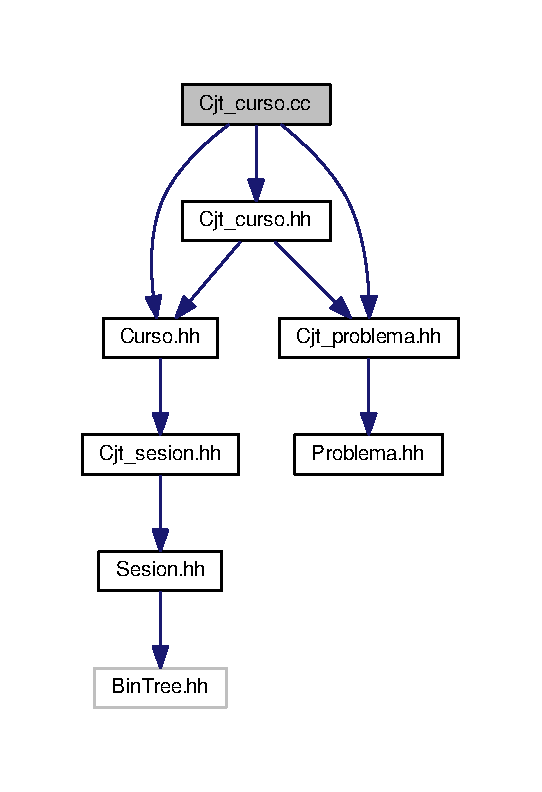
\includegraphics[width=260pt]{_cjt__curso_8cc__incl}
\end{center}
\end{figure}

\hypertarget{_cjt__curso_8hh}{}\section{Referencia del Archivo Cjt\+\_\+curso.\+hh}
\label{_cjt__curso_8hh}\index{Cjt\+\_\+curso.\+hh@{Cjt\+\_\+curso.\+hh}}


Especificacion de un conjunto de \mbox{\hyperlink{class_cjt__curso}{Cjt\+\_\+curso}}.  


Dependencia gráfica adjunta para Cjt\+\_\+curso.\+hh\+:
\nopagebreak
\begin{figure}[H]
\begin{center}
\leavevmode
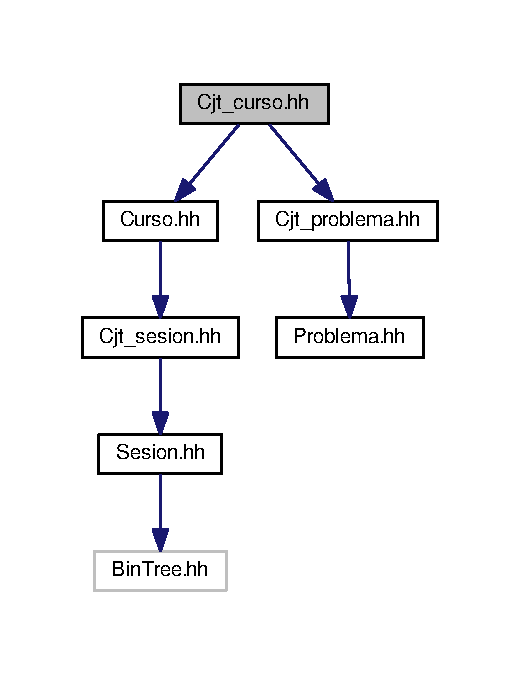
\includegraphics[width=250pt]{_cjt__curso_8hh__incl}
\end{center}
\end{figure}
\subsection*{Clases}
\begin{DoxyCompactItemize}
\item 
class \mbox{\hyperlink{class_cjt__curso}{Cjt\+\_\+curso}}
\begin{DoxyCompactList}\small\item\em Representa un conjunto de cursos. \end{DoxyCompactList}\end{DoxyCompactItemize}


\subsection{Descripción detallada}
Especificacion de un conjunto de \mbox{\hyperlink{class_cjt__curso}{Cjt\+\_\+curso}}. 


\hypertarget{_cjt__problema_8cc}{}\section{Referencia del Archivo Cjt\+\_\+problema.\+cc}
\label{_cjt__problema_8cc}\index{Cjt\+\_\+problema.\+cc@{Cjt\+\_\+problema.\+cc}}
Dependencia gráfica adjunta para Cjt\+\_\+problema.\+cc\+:
\nopagebreak
\begin{figure}[H]
\begin{center}
\leavevmode
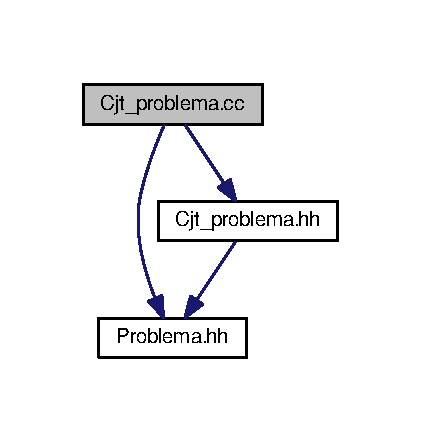
\includegraphics[width=202pt]{_cjt__problema_8cc__incl}
\end{center}
\end{figure}

\hypertarget{_cjt__problema_8hh}{}\section{Referencia del Archivo Cjt\+\_\+problema.\+hh}
\label{_cjt__problema_8hh}\index{Cjt\+\_\+problema.\+hh@{Cjt\+\_\+problema.\+hh}}


Especificacion de un conjunto de \mbox{\hyperlink{class_cjt__problema}{Cjt\+\_\+problema}}.  


Dependencia gráfica adjunta para Cjt\+\_\+problema.\+hh\+:
\nopagebreak
\begin{figure}[H]
\begin{center}
\leavevmode
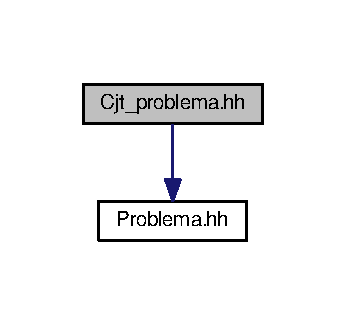
\includegraphics[width=166pt]{_cjt__problema_8hh__incl}
\end{center}
\end{figure}
\subsection*{Clases}
\begin{DoxyCompactItemize}
\item 
class \mbox{\hyperlink{class_cjt__problema}{Cjt\+\_\+problema}}
\begin{DoxyCompactList}\small\item\em Representa un conjunto de problemas. \end{DoxyCompactList}\end{DoxyCompactItemize}


\subsection{Descripción detallada}
Especificacion de un conjunto de \mbox{\hyperlink{class_cjt__problema}{Cjt\+\_\+problema}}. 


\hypertarget{_cjt__sesion_8cc}{}\section{Referencia del Archivo Cjt\+\_\+sesion.\+cc}
\label{_cjt__sesion_8cc}\index{Cjt\+\_\+sesion.\+cc@{Cjt\+\_\+sesion.\+cc}}
Dependencia gráfica adjunta para Cjt\+\_\+sesion.\+cc\+:
\nopagebreak
\begin{figure}[H]
\begin{center}
\leavevmode
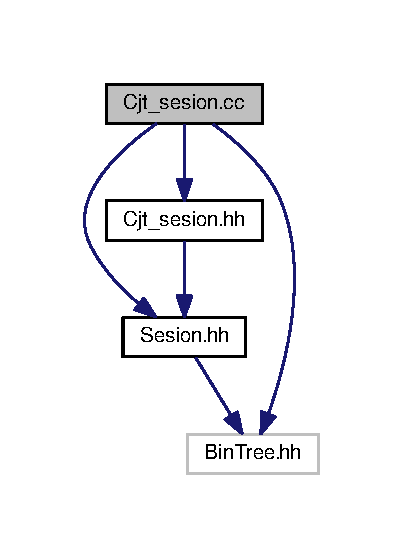
\includegraphics[width=193pt]{_cjt__sesion_8cc__incl}
\end{center}
\end{figure}

\hypertarget{_cjt__sesion_8hh}{}\section{Referencia del Archivo Cjt\+\_\+sesion.\+hh}
\label{_cjt__sesion_8hh}\index{Cjt\+\_\+sesion.\+hh@{Cjt\+\_\+sesion.\+hh}}


Especificacion de un conjunto de sesiones.  


Dependencia gráfica adjunta para Cjt\+\_\+sesion.\+hh\+:
\nopagebreak
\begin{figure}[H]
\begin{center}
\leavevmode
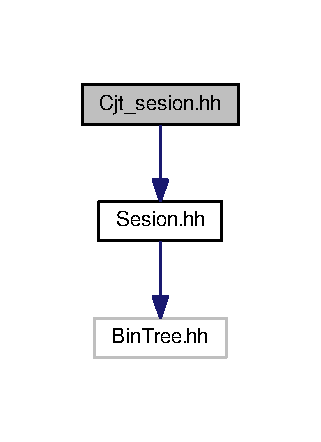
\includegraphics[width=154pt]{_cjt__sesion_8hh__incl}
\end{center}
\end{figure}
\subsection*{Clases}
\begin{DoxyCompactItemize}
\item 
class \mbox{\hyperlink{class_cjt__sesion}{Cjt\+\_\+sesion}}
\begin{DoxyCompactList}\small\item\em Representa un conjunto de sesiones. \end{DoxyCompactList}\end{DoxyCompactItemize}


\subsection{Descripción detallada}
Especificacion de un conjunto de sesiones. 


\hypertarget{_cjt__usuario_8cc}{}\section{Referencia del Archivo Cjt\+\_\+usuario.\+cc}
\label{_cjt__usuario_8cc}\index{Cjt\+\_\+usuario.\+cc@{Cjt\+\_\+usuario.\+cc}}
Dependencia gráfica adjunta para Cjt\+\_\+usuario.\+cc\+:
\nopagebreak
\begin{figure}[H]
\begin{center}
\leavevmode
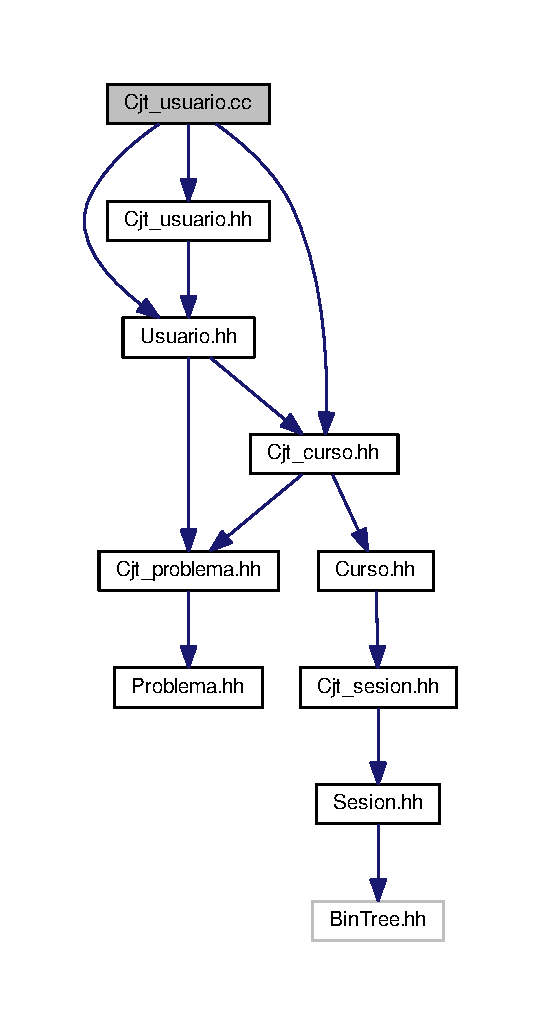
\includegraphics[width=259pt]{_cjt__usuario_8cc__incl}
\end{center}
\end{figure}

\hypertarget{_cjt__usuario_8hh}{}\section{Referencia del Archivo Cjt\+\_\+usuario.\+hh}
\label{_cjt__usuario_8hh}\index{Cjt\+\_\+usuario.\+hh@{Cjt\+\_\+usuario.\+hh}}


Especificacion de un conjunto de \mbox{\hyperlink{class_cjt__usuario}{Cjt\+\_\+usuario}}.  


Dependencia gráfica adjunta para Cjt\+\_\+usuario.\+hh\+:
\nopagebreak
\begin{figure}[H]
\begin{center}
\leavevmode
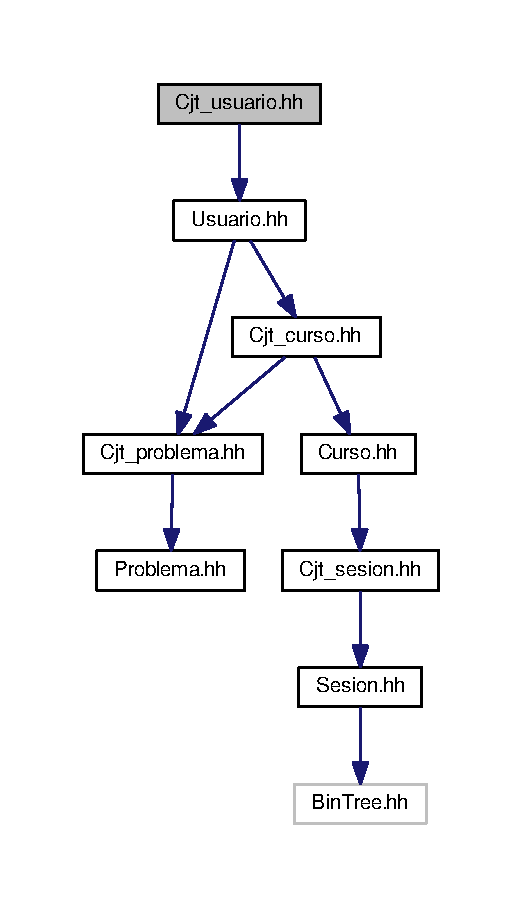
\includegraphics[width=250pt]{_cjt__usuario_8hh__incl}
\end{center}
\end{figure}
\subsection*{Clases}
\begin{DoxyCompactItemize}
\item 
class \mbox{\hyperlink{class_cjt__usuario}{Cjt\+\_\+usuario}}
\begin{DoxyCompactList}\small\item\em Representa un conjunto de usuarios. \end{DoxyCompactList}\end{DoxyCompactItemize}


\subsection{Descripción detallada}
Especificacion de un conjunto de \mbox{\hyperlink{class_cjt__usuario}{Cjt\+\_\+usuario}}. 


\hypertarget{_curso_8cc}{}\section{Referencia del Archivo Curso.\+cc}
\label{_curso_8cc}\index{Curso.\+cc@{Curso.\+cc}}
Dependencia gráfica adjunta para Curso.\+cc\+:
\nopagebreak
\begin{figure}[H]
\begin{center}
\leavevmode
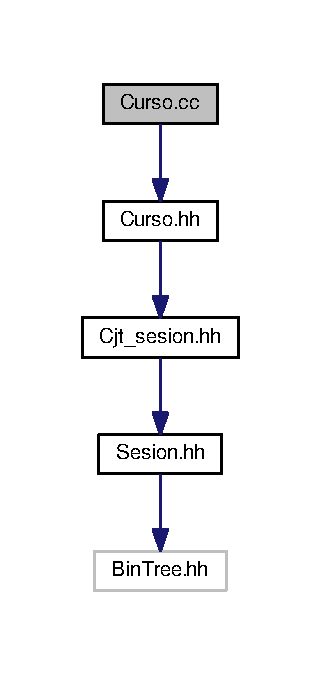
\includegraphics[width=154pt]{_curso_8cc__incl}
\end{center}
\end{figure}

\hypertarget{_curso_8hh}{}\section{Referencia del Archivo Curso.\+hh}
\label{_curso_8hh}\index{Curso.\+hh@{Curso.\+hh}}


Especificacion de curso.  


Dependencia gráfica adjunta para Curso.\+hh\+:
\nopagebreak
\begin{figure}[H]
\begin{center}
\leavevmode
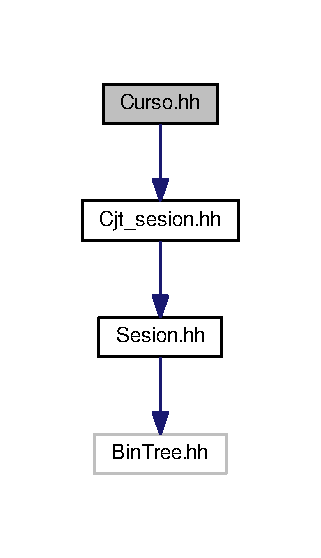
\includegraphics[width=154pt]{_curso_8hh__incl}
\end{center}
\end{figure}
\subsection*{Clases}
\begin{DoxyCompactItemize}
\item 
class \mbox{\hyperlink{class_curso}{Curso}}
\begin{DoxyCompactList}\small\item\em Representa un curso en la plataforma con un numero de sesiones y sus estadisticas de cuantos usuarios estan escritos y cuantos han completado el curso y un identificador unico. \end{DoxyCompactList}\end{DoxyCompactItemize}


\subsection{Descripción detallada}
Especificacion de curso. 


\hypertarget{_problema_8cc}{}\section{Referencia del Archivo Problema.\+cc}
\label{_problema_8cc}\index{Problema.\+cc@{Problema.\+cc}}
Dependencia gráfica adjunta para Problema.\+cc\+:
\nopagebreak
\begin{figure}[H]
\begin{center}
\leavevmode
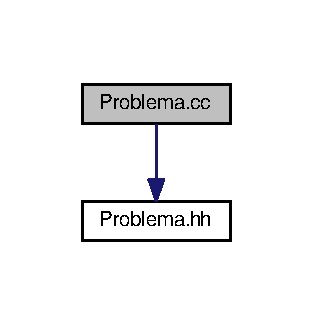
\includegraphics[width=150pt]{_problema_8cc__incl}
\end{center}
\end{figure}

\hypertarget{_problema_8hh}{}\section{Referencia del Archivo Problema.\+hh}
\label{_problema_8hh}\index{Problema.\+hh@{Problema.\+hh}}


Especificacion de problema.  


\subsection*{Clases}
\begin{DoxyCompactItemize}
\item 
class \mbox{\hyperlink{class_problema}{Problema}}
\begin{DoxyCompactList}\small\item\em Representa un problema en la plataforma con sus estadisticas de cuantos envios se han hecho, cuantos envios exitosos y el ratio de envios/envios\+\_\+exitosos del problema. Ademas de un identificador unico. \end{DoxyCompactList}\end{DoxyCompactItemize}


\subsection{Descripción detallada}
Especificacion de problema. 


\hypertarget{program_8cc}{}\section{Referencia del Archivo program.\+cc}
\label{program_8cc}\index{program.\+cc@{program.\+cc}}
Dependencia gráfica adjunta para program.\+cc\+:
\nopagebreak
\begin{figure}[H]
\begin{center}
\leavevmode
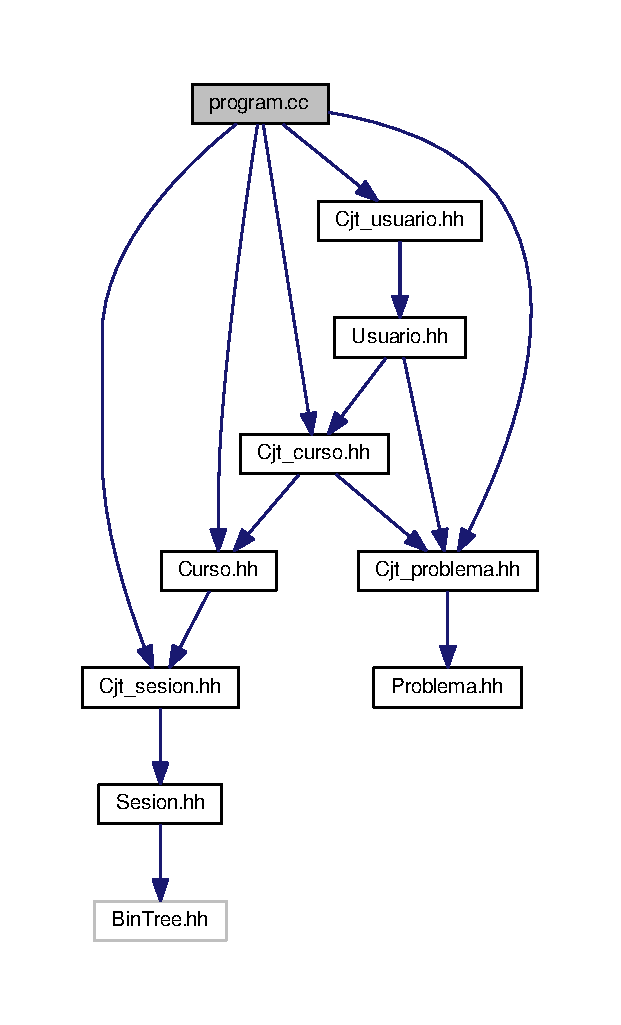
\includegraphics[width=298pt]{program_8cc__incl}
\end{center}
\end{figure}
\subsection*{Funciones}
\begin{DoxyCompactItemize}
\item 
int \mbox{\hyperlink{program_8cc_ae66f6b31b5ad750f1fe042a706a4e3d4}{main}} ()
\end{DoxyCompactItemize}


\subsection{Documentación de las funciones}
\mbox{\Hypertarget{program_8cc_ae66f6b31b5ad750f1fe042a706a4e3d4}\label{program_8cc_ae66f6b31b5ad750f1fe042a706a4e3d4}} 
\index{program.\+cc@{program.\+cc}!main@{main}}
\index{main@{main}!program.\+cc@{program.\+cc}}
\subsubsection{\texorpdfstring{main()}{main()}}
{\footnotesize\ttfamily int main (\begin{DoxyParamCaption}{ }\end{DoxyParamCaption})}



Definición en la línea 16 del archivo program.\+cc.


\begin{DoxyCode}
16            \{
17     \mbox{\hyperlink{class_cjt__problema}{Cjt\_problema}} lista\_problemas;
18     \textcolor{comment}{//leemos y guardamos todos los problemas}
19     \textcolor{keywordtype}{int} n;
20     \textcolor{comment}{//leemos y añadimos la cantidad de problemas a añadir a lista\_problemas}
21     cin >> n;
22     lista\_problemas.\mbox{\hyperlink{class_cjt__problema_afaff62599264105423f37fd1503cfb19}{leer\_problemas}}(n);
23 
24     \mbox{\hyperlink{class_cjt__sesion}{Cjt\_sesion}} lista\_sesiones;
25     \textcolor{comment}{//leemos y añadimos la cantidad de sesiones a añadir a lista\_sesones}
26     cin >> n;
27     lista\_sesiones.\mbox{\hyperlink{class_cjt__sesion_ad64b0e5339bd3a04de4fba88d6eb98c7}{leer\_sesiones}}(n);
28 
29     \mbox{\hyperlink{class_cjt__curso}{Cjt\_curso}} lista\_cursos;
30     \textcolor{comment}{//leemos y añadimos la cantidad de cursos a añadir a lista\_cursos}
31     cin >> n;
32     lista\_cursos.\mbox{\hyperlink{class_cjt__curso_a16e2b8c5304b5cb0562f95089f020a97}{leer\_cursos}}(n, lista\_sesiones);
33 
34 
35     \mbox{\hyperlink{class_cjt__usuario}{Cjt\_usuario}} lista\_usuarios;
36     \textcolor{comment}{//leemos y añadimos la cantidad de cursos a añadir a lista\_usuarios}
37     cin >> n;
38     lista\_usuarios.\mbox{\hyperlink{class_cjt__usuario_a75a98423be866287a841a77849ea3e6f}{leer\_usuarios}}(n);
39 
40     \textcolor{keywordtype}{string} comando;
41     \textcolor{comment}{//leemos el primer comando}
42     cin >> comando;
43     \textcolor{keywordflow}{while} (comando != \textcolor{stringliteral}{"fin"}) \{
44       \textcolor{keywordflow}{if} (comando == \textcolor{stringliteral}{"nuevo\_problema"} or comando == \textcolor{stringliteral}{"np"}) \{
45           \textcolor{keywordtype}{string} p; cin >> p;
46           cout << \textcolor{charliteral}{'#'} << comando << \textcolor{charliteral}{' '} << p << endl;
47           \textcolor{keywordflow}{try} \{
48               lista\_problemas.\mbox{\hyperlink{class_cjt__problema_a6086147f5615c1cf42d6d563682b080d}{anadir\_problema}}(p);
49               cout << lista\_problemas.\mbox{\hyperlink{class_cjt__problema_acf0fca6955f991a9debb4ef50ece8905}{num\_problemas}}() << endl;
50           \} \textcolor{keywordflow}{catch} (\textcolor{keyword}{const} \textcolor{keywordtype}{char}* msg) \{
51               cout << \textcolor{stringliteral}{"error: "} << msg << endl;
52           \}
53       \}
54       \textcolor{keywordflow}{if} (comando == \textcolor{stringliteral}{"nueva\_sesion"} or comando == \textcolor{stringliteral}{"ns"}) \{
55           \textcolor{keywordtype}{string} s; cin >> s;
56           cout << \textcolor{charliteral}{'#'} << comando << \textcolor{charliteral}{' '} << s << endl;
57           \textcolor{keywordflow}{try} \{
58               lista\_sesiones.\mbox{\hyperlink{class_cjt__sesion_ace504b799e2c370749ccb16f9312fa5f}{anadir\_sesion}}(s);
59               cout << lista\_sesiones.\mbox{\hyperlink{class_cjt__sesion_aa885f9672e699d82dcd22aaa26d1ada8}{num\_sesiones}}() << endl;
60           \} \textcolor{keywordflow}{catch} (\textcolor{keyword}{const} \textcolor{keywordtype}{char}* msg) \{
61               cout << \textcolor{stringliteral}{"error: "} << msg << endl;
62           \}
63       \}
64       \textcolor{keywordflow}{if} (comando == \textcolor{stringliteral}{"nuevo\_curso"} or comando == \textcolor{stringliteral}{"nc"}) \{
65           cout << \textcolor{charliteral}{'#'} << comando << endl;
66           \textcolor{keywordflow}{try} \{
67               \mbox{\hyperlink{class_curso}{Curso}} c;
68               \textcolor{comment}{//leer sesiones del curso comporbando que no se solapen}
69               c.\mbox{\hyperlink{class_curso_ad60de4c73f3ce9195c0f681f508f83c8}{leer\_sesiones}}(lista\_sesiones);
70               \textcolor{comment}{//se añade el curso a lista\_cursos (crear funcion para añadir objetos)}
71               lista\_cursos.\mbox{\hyperlink{class_cjt__curso_a8b79841cba9bb04c08a23e9dc376dd24}{anadir\_curso}}(c);
72               \textcolor{comment}{//se imprime el idetificador}
73               cout << lista\_cursos.\mbox{\hyperlink{class_cjt__curso_a1ad84838189a13e86741d96cf2107d9c}{num\_cursos}}() << endl;
74           \} \textcolor{keywordflow}{catch} (\textcolor{keyword}{const} \textcolor{keywordtype}{char}* msg) \{
75               cout << \textcolor{stringliteral}{"error: "} << msg << endl;
76           \}
77       \}
78       \textcolor{keywordflow}{if} (comando == \textcolor{stringliteral}{"alta\_usuario"} or comando == \textcolor{stringliteral}{"a"}) \{
79           \textcolor{keywordtype}{string} u; cin >> u;
80           cout << \textcolor{charliteral}{'#'} << comando << \textcolor{charliteral}{' '} << u << endl;
81           \textcolor{keywordflow}{try} \{
82               lista\_usuarios.\mbox{\hyperlink{class_cjt__usuario_a1a587cd6e8e3f261f27981134d0216e5}{anadir\_usuario}}(u);
83               cout << lista\_usuarios.\mbox{\hyperlink{class_cjt__usuario_a92ec4442d4a6e8d50f4eb36413ade07e}{num\_usuarios}}() << endl;
84           \} \textcolor{keywordflow}{catch} (\textcolor{keyword}{const} \textcolor{keywordtype}{char}* msg) \{
85               cout << \textcolor{stringliteral}{"error: "} << msg << endl;
86           \}
87       \}
88       \textcolor{keywordflow}{if} (comando == \textcolor{stringliteral}{"baja\_usuario"} or comando == \textcolor{stringliteral}{"b"}) \{
89           \textcolor{keywordtype}{string} u; cin >> u;
90             cout << \textcolor{charliteral}{'#'} << comando << \textcolor{charliteral}{' '} << u << endl;
91           \textcolor{keywordflow}{try} \{
92               lista\_usuarios.\mbox{\hyperlink{class_cjt__usuario_a4be0bd7bbca32d299b152730d6de41ba}{eliminar\_usuario}}(u, lista\_cursos);
93               cout << lista\_usuarios.\mbox{\hyperlink{class_cjt__usuario_a92ec4442d4a6e8d50f4eb36413ade07e}{num\_usuarios}}() << endl;
94           \} \textcolor{keywordflow}{catch} (\textcolor{keyword}{const} \textcolor{keywordtype}{char}* msg) \{
95               cout << \textcolor{stringliteral}{"error: "} << msg << endl;
96           \}
97       \}
98       \textcolor{keywordflow}{if} (comando == \textcolor{stringliteral}{"inscribir\_curso"} or comando == \textcolor{stringliteral}{"i"}) \{
99           \textcolor{keywordtype}{string} u; \textcolor{keywordtype}{int} c; cin >> u >> c;
100           cout << \textcolor{charliteral}{'#'} << comando << \textcolor{charliteral}{' '} << u << \textcolor{charliteral}{' '} << c << endl;
101           \textcolor{keywordflow}{try} \{
102                lista\_usuarios.\mbox{\hyperlink{class_cjt__usuario_a3f4be6c8f5568ef3767bf343418e6f5d}{inscribir\_curso}}(u, c, lista\_cursos, lista\_sesiones);
103                lista\_cursos.\mbox{\hyperlink{class_cjt__curso_ae5cf07c6e8883a244c7557e446490254}{inscribir\_usuario}}(c);
104                cout << lista\_cursos.\mbox{\hyperlink{class_cjt__curso_ac160a24d24ca6a57b7e8bf6925b10343}{num\_inscritos}}(c) << endl;
105 
106           \} \textcolor{keywordflow}{catch} (\textcolor{keyword}{const} \textcolor{keywordtype}{char}* msg) \{
107               cout << \textcolor{stringliteral}{"error: "} << msg << endl;
108           \}
109       \}
110       \textcolor{keywordflow}{if} (comando == \textcolor{stringliteral}{"curso\_usuario"} or comando == \textcolor{stringliteral}{"cu"}) \{
111           \textcolor{keywordtype}{string} u; cin >> u;
112           cout << \textcolor{charliteral}{'#'} << comando << \textcolor{charliteral}{' '} << u << endl;
113           \textcolor{keywordflow}{try} \{
114                cout << lista\_usuarios.\mbox{\hyperlink{class_cjt__usuario_aa21aa736c5b2094fe5d21415f1761cfa}{curso\_actual}}(u) << endl;
115           \} \textcolor{keywordflow}{catch} (\textcolor{keyword}{const} \textcolor{keywordtype}{char}* msg) \{
116               cout << \textcolor{stringliteral}{"error: "} << msg << endl;
117           \}
118       \}
119       \textcolor{keywordflow}{if} (comando == \textcolor{stringliteral}{"sesion\_problema"} or comando == \textcolor{stringliteral}{"sp"}) \{
120           \textcolor{keywordtype}{string} p; \textcolor{keywordtype}{int} c; cin >> c >> p;
121           cout << \textcolor{charliteral}{'#'} << comando << \textcolor{charliteral}{' '} << c << \textcolor{charliteral}{' '} << p << endl;
122           \textcolor{keywordflow}{try} \{
123                cout << lista\_cursos.\mbox{\hyperlink{class_cjt__curso_a6d9976b271bd773bdff14e79991231e4}{consultar\_sesion\_problema}}(p, c, 
      lista\_problemas) << endl;
124           \} \textcolor{keywordflow}{catch} (\textcolor{keyword}{const} \textcolor{keywordtype}{char}* msg) \{
125               cout << \textcolor{stringliteral}{"error: "} << msg << endl;
126           \}
127       \}
128       \textcolor{keywordflow}{if} (comando == \textcolor{stringliteral}{"problemas\_resueltos"} or comando == \textcolor{stringliteral}{"pr"}) \{
129           \textcolor{keywordtype}{string} u; cin >> u;
130           cout << \textcolor{charliteral}{'#'} << comando << \textcolor{charliteral}{' '} << u << endl;
131           \textcolor{keywordflow}{try} \{
132                lista\_usuarios.\mbox{\hyperlink{class_cjt__usuario_aa1cfea5c4294317758f260033f9fbd3f}{problemas\_resueltos}}(u);
133           \} \textcolor{keywordflow}{catch} (\textcolor{keyword}{const} \textcolor{keywordtype}{char}* msg) \{
134               cout << \textcolor{stringliteral}{"error: "} << msg << endl;
135           \}
136       \}
137       \textcolor{keywordflow}{if} (comando == \textcolor{stringliteral}{"problemas\_enviables"} or comando == \textcolor{stringliteral}{"pe"}) \{
138           \textcolor{keywordtype}{string} u; cin >> u;
139           cout << \textcolor{charliteral}{'#'} << comando << \textcolor{charliteral}{' '} << u << endl;
140           \textcolor{keywordflow}{try} \{
141                lista\_usuarios.\mbox{\hyperlink{class_cjt__usuario_adf8f61c7eacd7328896c168adb3e63cd}{problemas\_enviables}}(u);
142           \} \textcolor{keywordflow}{catch} (\textcolor{keyword}{const} \textcolor{keywordtype}{char}* msg) \{
143               cout << \textcolor{stringliteral}{"error: "} << msg << endl;
144           \}
145       \}
146       \textcolor{keywordflow}{if} (comando == \textcolor{stringliteral}{"envio"} or comando == \textcolor{stringliteral}{"e"}) \{
147           \textcolor{keywordtype}{string} u, p; \textcolor{keywordtype}{int} r; cin >> u >> p >> r;
148           cout << \textcolor{charliteral}{'#'} << comando << \textcolor{charliteral}{' '} << u << \textcolor{charliteral}{' '} << p << \textcolor{charliteral}{' '} << r << endl;
149           \textcolor{keywordflow}{try} \{
150             lista\_usuarios.\mbox{\hyperlink{class_cjt__usuario_a239dce70ba54f8a8f41fd180b703b7c9}{envio\_user}}(u, p, r, lista\_problemas, lista\_cursos, lista\_sesiones);
151           \} \textcolor{keywordflow}{catch} (\textcolor{keyword}{const} \textcolor{keywordtype}{char}* msg) \{
152               cout << \textcolor{stringliteral}{"error: "} << msg << endl;
153           \}
154       \}
155       \textcolor{keywordflow}{if} (comando == \textcolor{stringliteral}{"listar\_problemas"} or comando == \textcolor{stringliteral}{"lp"}) \{
156         cout << \textcolor{charliteral}{'#'} << comando << endl;
157           \textcolor{keywordflow}{try} \{
158             lista\_problemas.\mbox{\hyperlink{class_cjt__problema_a4966292b86b69ab0fef01154e79aeb54}{listar\_problemas}}();
159           \} \textcolor{keywordflow}{catch} (\textcolor{keyword}{const} \textcolor{keywordtype}{char}* msg) \{
160               cout << \textcolor{stringliteral}{"error: "} << msg << endl;
161           \}
162       \}
163       \textcolor{keywordflow}{if} (comando == \textcolor{stringliteral}{"escribir\_problema"} or comando == \textcolor{stringliteral}{"ep"}) \{
164           \textcolor{keywordtype}{string} p; cin >> p;
165           cout << \textcolor{charliteral}{'#'} << comando << \textcolor{charliteral}{' '} << p << endl;
166           \textcolor{keywordflow}{try} \{
167             lista\_problemas.\mbox{\hyperlink{class_cjt__problema_a72e742fbaa5618065f2e478b59bf3036}{listar\_problema}}(p);
168           \} \textcolor{keywordflow}{catch} (\textcolor{keyword}{const} \textcolor{keywordtype}{char}* msg) \{
169               cout << \textcolor{stringliteral}{"error: "} << msg << endl;
170           \}
171       \}
172       \textcolor{keywordflow}{if} (comando == \textcolor{stringliteral}{"listar\_sesiones"} or comando == \textcolor{stringliteral}{"ls"}) \{
173         cout << \textcolor{charliteral}{'#'} << comando << endl;
174           \textcolor{keywordflow}{try} \{
175               lista\_sesiones.\mbox{\hyperlink{class_cjt__sesion_ab16589173601c81f80305cd9a49b2f7b}{listar\_sesiones}}();
176           \} \textcolor{keywordflow}{catch} (\textcolor{keyword}{const} \textcolor{keywordtype}{char}* msg) \{
177               cout << \textcolor{stringliteral}{"error: "} << msg << endl;
178           \}
179       \}
180       \textcolor{keywordflow}{if} (comando == \textcolor{stringliteral}{"escribir\_sesion"} or comando == \textcolor{stringliteral}{"es"}) \{
181           \textcolor{keywordtype}{string} s; cin >> s;
182           cout << \textcolor{charliteral}{'#'} << comando << \textcolor{charliteral}{' '} << s << endl;
183           \textcolor{keywordflow}{try} \{
184             lista\_sesiones.\mbox{\hyperlink{class_cjt__sesion_a8d8d2ba30c0efeb90e21a9b41fa2c62e}{listar\_sesion}}(s);
185           \} \textcolor{keywordflow}{catch} (\textcolor{keyword}{const} \textcolor{keywordtype}{char}* msg) \{
186               cout << \textcolor{stringliteral}{"error: "} << msg << endl;
187           \}
188       \}
189       \textcolor{keywordflow}{if} (comando == \textcolor{stringliteral}{"listar\_cursos"} or comando == \textcolor{stringliteral}{"lc"}) \{
190         cout << \textcolor{charliteral}{'#'} << comando << endl;
191           \textcolor{keywordflow}{try} \{
192               lista\_cursos.\mbox{\hyperlink{class_cjt__curso_a2a1a2f9d0f54afaf5239b661f0d74164}{listar\_cursos}}();
193           \} \textcolor{keywordflow}{catch} (\textcolor{keyword}{const} \textcolor{keywordtype}{char}* msg) \{
194               cout << \textcolor{stringliteral}{"error: "} << msg << endl;
195           \}
196       \}
197       \textcolor{keywordflow}{if} (comando == \textcolor{stringliteral}{"escribir\_curso"} or comando == \textcolor{stringliteral}{"ec"}) \{
198           \textcolor{keywordtype}{int} c; cin >> c;
199           cout << \textcolor{charliteral}{'#'} << comando << \textcolor{charliteral}{' '} << c << endl;
200           \textcolor{keywordflow}{try} \{
201             lista\_cursos.\mbox{\hyperlink{class_cjt__curso_a8757e2e3a01006da2a553e9fbf119fd9}{listar\_curso}}(c);
202           \} \textcolor{keywordflow}{catch} (\textcolor{keyword}{const} \textcolor{keywordtype}{char}* msg) \{
203               cout << \textcolor{stringliteral}{"error: "} << msg << endl;
204           \}
205       \}
206       \textcolor{keywordflow}{if} (comando == \textcolor{stringliteral}{"listar\_usuarios"} or comando == \textcolor{stringliteral}{"lu"}) \{
207         cout << \textcolor{charliteral}{'#'} << comando << endl;
208           \textcolor{keywordflow}{try} \{
209               lista\_usuarios.\mbox{\hyperlink{class_cjt__usuario_a4cd3e0812c3b3d7e9e83c0f8d0c2acb3}{listar\_usuarios}}();
210           \} \textcolor{keywordflow}{catch} (\textcolor{keyword}{const} \textcolor{keywordtype}{char}* msg) \{
211               cout << \textcolor{stringliteral}{"error: "} << msg << endl;
212           \}
213       \}
214       \textcolor{keywordflow}{if} (comando == \textcolor{stringliteral}{"escribir\_usuario"} or comando == \textcolor{stringliteral}{"eu"}) \{
215           \textcolor{keywordtype}{string} u; cin >> u;
216           cout << \textcolor{charliteral}{'#'} << comando << \textcolor{charliteral}{' '} << u << endl;
217           \textcolor{keywordflow}{try} \{
218             lista\_usuarios.\mbox{\hyperlink{class_cjt__usuario_aa1b390ae2335eb486d2a0c8c32643d5c}{listar\_usuario}}(u);
219           \} \textcolor{keywordflow}{catch} (\textcolor{keyword}{const} \textcolor{keywordtype}{char}* msg) \{
220               cout << \textcolor{stringliteral}{"error: "} << msg << endl;
221           \}
222       \}
223       cin >> comando;
224     \}
225 \}
\end{DoxyCode}

\hypertarget{_sesion_8cc}{}\section{Referencia del Archivo Sesion.\+cc}
\label{_sesion_8cc}\index{Sesion.\+cc@{Sesion.\+cc}}
Dependencia gráfica adjunta para Sesion.\+cc\+:
\nopagebreak
\begin{figure}[H]
\begin{center}
\leavevmode
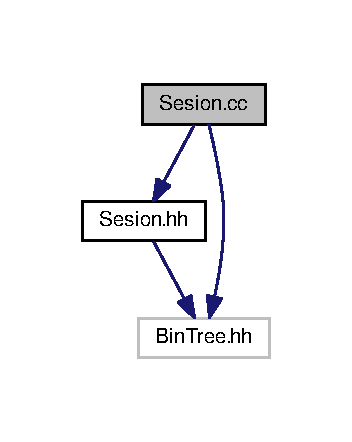
\includegraphics[width=169pt]{_sesion_8cc__incl}
\end{center}
\end{figure}

\hypertarget{_sesion_8hh}{}\section{Referencia del Archivo Sesion.\+hh}
\label{_sesion_8hh}\index{Sesion.\+hh@{Sesion.\+hh}}


Especificacion de sesion.  


Dependencia gráfica adjunta para Sesion.\+hh\+:
\nopagebreak
\begin{figure}[H]
\begin{center}
\leavevmode
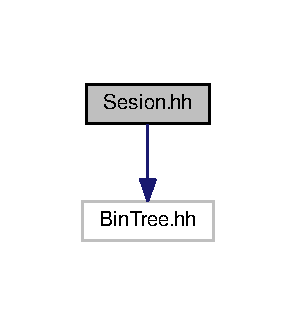
\includegraphics[width=142pt]{_sesion_8hh__incl}
\end{center}
\end{figure}
\subsection*{Clases}
\begin{DoxyCompactItemize}
\item 
class \mbox{\hyperlink{class_sesion}{Sesion}}
\begin{DoxyCompactList}\small\item\em Representa una sesion de la plataforma con un arbol binario indicando los pre requisitos para poder realizar un envio a un problema, un mapa con todos los problemas y un identificador unico. \end{DoxyCompactList}\end{DoxyCompactItemize}


\subsection{Descripción detallada}
Especificacion de sesion. 


\hypertarget{_usuario_8cc}{}\section{Referencia del Archivo Usuario.\+cc}
\label{_usuario_8cc}\index{Usuario.\+cc@{Usuario.\+cc}}
Dependencia gráfica adjunta para Usuario.\+cc\+:
\nopagebreak
\begin{figure}[H]
\begin{center}
\leavevmode
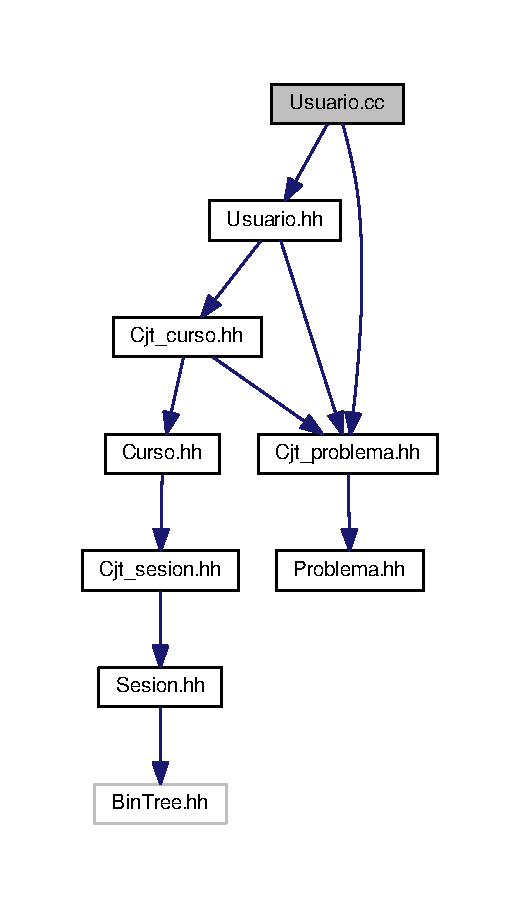
\includegraphics[width=250pt]{_usuario_8cc__incl}
\end{center}
\end{figure}

\hypertarget{_usuario_8hh}{}\section{Referencia del Archivo Usuario.\+hh}
\label{_usuario_8hh}\index{Usuario.\+hh@{Usuario.\+hh}}


Especificacion de usuario.  


Dependencia gráfica adjunta para Usuario.\+hh\+:
\nopagebreak
\begin{figure}[H]
\begin{center}
\leavevmode
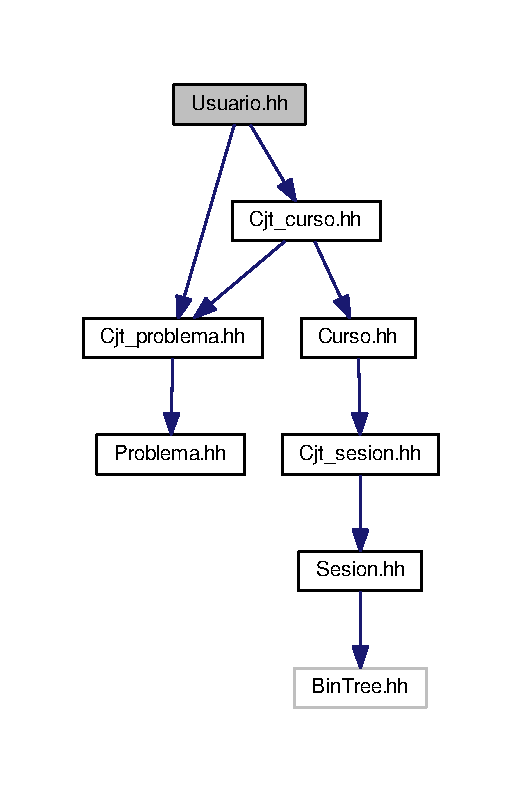
\includegraphics[width=250pt]{_usuario_8hh__incl}
\end{center}
\end{figure}
\subsection*{Clases}
\begin{DoxyCompactItemize}
\item 
class \mbox{\hyperlink{class_usuario}{Usuario}}
\begin{DoxyCompactList}\small\item\em Representa un usuario en la plataforma con sus estadisticas de cuantos envios se han hecho, cuantos problemas se han intenado hacer, ademas del curso al que esta inscrito dicho usuario, un identificador unico y dos conjuntos con los problemas que puede enviar y los que ya ha resuelto. \end{DoxyCompactList}\end{DoxyCompactItemize}


\subsection{Descripción detallada}
Especificacion de usuario. 


%--- End generated contents ---

% Index
\backmatter
\newpage
\phantomsection
\clearemptydoublepage
\addcontentsline{toc}{chapter}{Índice}
\printindex

\end{document}
